% arara: xelatex: { shell: yes, synctex: yes }
\documentclass[english,fira]{ist-report}

%\usepackage{geometry}
\usepackage{xcolor}
\usepackage{hyperref}
\usepackage{amsmath}
\usepackage{amssymb}
\usepackage[sfdefault]{FiraSans}
\renewcommand*\oldstylenums[1]{{\firaoldstyle #1}}
\usepackage[mathrm = sym]{unicode-math}
\setmathfont[
    %Path = ./fonts/,
    Extension = .otf]{FiraMath-Regular}
\usepackage{FiraMono}

\renewcommand{\baselinestretch}{1.15}

\geometry{top=1cm}
\settitle{Aerospace Design}

% -- Bibliography
\usepackage{csquotes}
\usepackage{biblatex}
\addbibresource{main.bib}

% -- Extra math options
%\usepackage{mathtools}
\usepackage{siunitx}
\DeclareSIUnit\rpm{rpm}
\DeclareSIUnit\rps{rps}
\DeclareSIUnit\foot{ft}
\DeclareSIUnit\inch{in}
\DeclareSIUnit\ounce{oz}
\DeclareSIUnit\pound{lb}

% -- Extra symbols
\usepackage{amssymb}
\usepackage{textcomp}
\usepackage{gensymb}
\usepackage{cancel}

% -- Glossaries
\usepackage[toc,symbols]{glossaries-extra}
\usepackage{tocbibind}

% -- Additional table features
\usepackage{booktabs}
\usepackage{makecell}

% --  Image and float settings
\graphicspath{{graphics/}}
\usepackage{caption}
\usepackage{subcaption}
\usepackage{pdfpages}

% -- Graphs and diagrams
\usepackage{tikz}
\usepackage{pgfplots}
\usetikzlibrary{arrows.meta,positioning,patterns}
\pgfplotsset{compat=1.5, table/search path = {data}}

\newcolumntype{C}{>{$}c<{$}}


\DeclareTextCommandDefault{\nobreakspace}{\leavevmode\nobreak\ } 
\newcommand\micropilot{$\text{MP}2128^{\text{HELI}2}$}
\newrobustcmd*{\vnd}{$V$-$n$}
%\renewcommand{\baselinestretch}{1.15}

\newabbreviation{uav}{UAV}{Unmanned Aerial Vehicle}
\newabbreviation{icao}{ICAO}{International Civil Aviation Organization}
\newabbreviation{naca}{NACA}{National Advisory Committee for Aeronautics}
\newabbreviation{cad}{CAD}{Computer Aided Design}
\newabbreviation{vtol}{VTOL}{Vertical Take-Off and Landing}
\newabbreviation{ctol}{CTOL}{Conventional Take-Off and Landing}
\newabbreviation{stol}{STOL}{Short Take-Off and Landing}
\newabbreviation{stovl}{STOVL}{Short Take-Off and Vertical Landing}
\newabbreviation{rpv}{RPV}{Remotely Pilot Vehicle}
\newabbreviation{mad}{MAD}{Magnetic Anomaly Detection}
\newabbreviation{mtow}{MTOW}{Maximum Take-Off Weight}
\newabbreviation{kari}{KARI}{Korea Aerospace Research Institute}
\newabbreviation{ahp}{AHP}{Analytic Hierarchy Process}
\newabbreviation{fom}{FoM}{Figure of Merit}
\newabbreviation{faa}{FAA}{Federal Aviation Administration}
\newabbreviation{far}{FAR}{Federal Aviation Regulations}
\newabbreviation{gps}{GPS}{Global Positioning System}
\newabbreviation{gnss}{GNSS}{Global Navigation Satellite System}
\newabbreviation{lidar}{LIDAR}{Light Detection And Ranging}
\newabbreviation{cg}{CG}{Centre of gravity}
\newabbreviation{swil}{SWIL}{Software-In-The-Loop}

\newglossaryentry{density}{
    name        = {$\rho$},
    sort        = {rho},
    description = {Static density},
    type        = {symbols}
}

\newglossaryentry{ddensity}{
    name        = {$q$},
    sort        = {q},
    description = {Dynamic density},
    type        = {symbols}
}

\newglossaryentry{force}{
    name        = {$F$},
    sort        = {force},
    description = {Generic force},
    type        = {symbols}
}

\newglossaryentry{liftforce}{
    name        = {$L$},
    sort        = {forcel},
    description = {Lift force},
    type        = {symbols}
}

\newglossaryentry{dragforce}{
    name        = {$D$},
    sort        = {forced},
    description = {Drag force},
    type        = {symbols}
}

\newglossaryentry{weightforce}{
    name        = {$W$},
    sort        = {forcew},
    description = {Weight},
    type        = {symbols}
}

\newglossaryentry{notavailable}{
    name        = {n/a},
    sort        = {na},
    description = {Not available},
    type        = {symbols}
}

\newglossaryentry{wingspan}{
    name        = {$b$},
    sort        = {b},
    description = {Wing span},
    type        = {symbols}
}

\newglossaryentry{mach}{
    name        = {$M$},
    sort        = {mach},
    description = {Mach number},
    type        = {symbols}
}

\newglossaryentry{chord}{
    name        = {$c$},
    sort        = {chord},
    description = {Chord length},
    type        = {symbols}
}

\newglossaryentry{meanchord}{
    name        = {$\bar{c}$},
    sort        = {chord},
    description = {Mean chord length},
    type        = {symbols}
}

\newglossaryentry{taperratio}{
    name        = {$\lambda$},
    sort        = {lambda},
    description = {Taper ratio},
    type        = {symbols}
}

\newglossaryentry{aspectratio}{
    name        = {$AR$},
    sort        = {ar},
    description = {Aspect ratio},
    type        = {symbols}
}

\newglossaryentry{dviscosity}{
    name        = {$\mu$},
    sort        = {u},
    description = {Dynamic viscosity},
    type        = {symbols}
}

\newglossaryentry{kviscosity}{
    name        = {$\nu$},
    sort        = {v},
    description = {Kinematic viscosity},
    type        = {symbols}
}

\newglossaryentry{aoa}{
    name        = {$\alpha$},
    sort        = {alpha},
    description = {Angle of attack},
    type        = {symbols}
}

\newglossaryentry{gravity}{
    name        = {$g$},
    sort        = {gravity},
    description = {Surface gravity (usually $g = \SI{9.80665}{\meter\per\second\squared}$)},
    type        = {symbols}
}

\newglossaryentry{wingarea}{
    name        = {$S$},
    sort        = {surface},
    description = {Wing surface area},
    type        = {symbols}
}

\newglossaryentry{liftcoefficient}{
    name        = {$C_L$},
    sort        = {cl},
    description = {Lift coefficient},
    type        = {symbols}
}

\newglossaryentry{dragcoefficient}{
    name        = {$C_D$},
    sort        = {cd},
    description = {Drag coefficient},
    type        = {symbols}
}
\makeglossaries

\begin{document}

%\includepdf[pages = -, fitpaper = true]{ist-capa.pdf}
\thispagestyle{empty}


\includegraphics[viewport=9.5cm 11cm 0cm 0cm,scale=0.29]{IST_A_CMYK_POS}
	
\begin{center}
	\vspace{40mm} % --  Espaço em branco
	%\rule{\linewidth}{0.5pt} \\
    \vspace{2mm}
	{\Huge\bfseries Aerospace Design Project} \\
	%\rule{\linewidth}{2pt} \\
	\vspace{5mm} % -- Espaço em branco
	{\Large Development of a Vertical Take-Off and Landing UAV aircraft for use with magnetic sensors}
	
	\vspace{\fill} % --  Espaço em branco variável
	
	\normalsize
	\begin{tabular}{r l|}
		Tiago \textsc{Oliveira} & \textbf{81024} \\
		Carolina \textsc{Serra} & \textbf{80768} \\
		João \textsc{Rodrigues} & \textbf{81540} \\
		Daniel \textsc{de Schiffart} & \textbf{81479} \\
		Cristiano \textsc{Mesquita} & \textbf{81430} \\
		Julian \textsc{Stemmermann} & \textbf{91965}
	\end{tabular}\hspace*{2mm} {\Large Group 7}
	
	%\medskip
	%{\Large\bfseries Group 7}
	
	\vspace{10mm} % --  Espaço em branco
	\Large Instituto Superior Técnico \\
	Integrated Master's Degree in Aerospace Engineering \\
	\vspace{1mm}
	\large Aerospace Design
	
	\vspace{10mm} % --  Espaço em branco
	\Large 2018/2019
\end{center}

\pagebreak


\begin{abstract}
    The project and its goal surround the study, design and projection of a fixed-wing vertical take-off and landing unmanned aerial vehicle, henceforth shortened to fixed-wing VTOL UAV, and its feasibility as a magnetic anomaly detection tool with the implementation of magnetometers within its hull \cite{proj_desc}. The focus of the study is directed to the implementation of said magnetometers and their interaction with the UAV's internal mechanical and electronic components and the magnetic noise thereby generated, and the effect of said noise on the magnetometers and the results captured by the same. Very careful consideration is given to the positioning of the magnetometers on the UAV's structure so as to minimise the captured aircraft-generated magnetic noise.
\end{abstract}

{\hypersetup{linkcolor = {black}}
    \tableofcontents
    \listoffigures
    \listoftables
    \glsaddall
    \printglossary[nogroupskip,nonumberlist]
    \printglossary[type=symbols,nogroupskip,nonumberlist]
}

\chapter{Overview}

The topics of focus throughout the development of the project are hereby listed and further presented. These topics represent the characteristic nuances of the projected aircraft in contrast with more standard configurations for the same topic, and are the focus of study in the development of the project.

\section{Unmanned Aerial Vehicle}

An unmanned aerial vehicle, also referred to as unmanned aircraft system, unmanned aircraft, or drone, henceforth referred to as UAV, is the name given to any aircraft that flies without a human pilot aboard during its operations. A UAV can be controlled through various methods, from being manually remotely piloted\footnotemark{} to fully autonomous navigation. According to the International Civil Aviation Organization \cite{icao_uav}, a UAV is defined as follows.
\begin{quotation} \itshape
    An unmanned aerial vehicle is a pilot-less aircraft, in the sense of Article 8 of the Convention on International Civil Aviation, which is flown without a pilot-in-command on-board and is either remotely and fully controlled from another place (ground, another aircraft, space) or programmed and fully autonomous.
\end{quotation}
\footnotetext{A remotely piloted UAV is referred to as an RPV, or Remotely Piloted Vehicle.}
While historically the first and foremost objective of heavier-that-air flight was to transport human passengers through the air, for motives ranging from transportation to reconnaissance to warfare, the widening of possibilities and uses for flight operations, in combination with the development of aircraft telemetry, communication and control technology has led to the widespread adoption of UAVs in many fields of engineering whenever the situation permits, leading to lower costs and less human risk involved in contrast to any manned aerial operations.

\section{Vertical Take-Off and Landing}

An aircraft that can a take-off and land vertically carries a VTOL, which stands for Vertical Take-Off and Landing. Other similar tags applied to aircraft depending on their take-off and landing methods include CTOL (Conventional Take-Off and Landing), STOL (Short Take-Off and Landing), and a mix of the previous modes.

The most prominent aircraft type included in the VTOL category are helicopters, whose propulsion method is aligned vertically to allow for this take-off method. Most fixed-wing aircraft are included in the CTOL category, but the presence of VTOL, STOL and STOVL (Short Take-Off and Vertical Landing) fixed-wing aircraft is well established, resorting to unconventional engine setups and additional propulsion methods to achieve this feat. The designation for this method of take-off and landing is \textbf{powered-lift}, as opposed to \textbf{rotorcraft}, which is used to describe the take-off and landing of helicopters and aircraft with similar configurations such as quadcopters.

\section{Magnetometry and Aviation}

Magnetometry focuses on the analysis of the changes of the magnetic field within a region, and to detect anomalies within said field. The range of applications of measuring the magnetic field and its change varies, often depending on its scale, from short-range metal detectors to wide-scale mapping of the Earth's magnetic field. For larger applications, such as the latter, the use of aircraft proved a natural pairing given the distance covered within a smaller time span compared to other options for transportation.

The use of aviation for magnetic measurement applications isn't a new concept. Historically there have been multiple cases of magnetic measurement missions being used for various applications, namely warfare, where they were used to detect submarines where eyesight proved unreliable or inadequate. These historical uses often relied on full-scale aircraft with passengers onboard, and depending on the age of the aircraft used, required less consideration of the onboard instruments as sources of noise for magnetic measurements. However, with the development of onboard systems and increase in the number of noise sources within most aircraft, and the emergence of smaller UAVs in modern aviation, obtaining clean and reliable magnetic measurements has proven to be more of a challenge as magnetic noise produced by the aircraft itself can, more and more, cause interference with the magnetic field obtained by its sensors.

Each aircraft has its own \textit{magnetic signature}, which equates to the magnetic noise generated by its internal components, with multiple different sources within the same aircraft \cite{mag_thesis}. This noise interferes with the data acquired by the magnetometers onboard and distorts the data obtained with varying intensity, with the objective of planning being to reduce this distortion as much as possible, ideally to negligible levels.

\chapter{Mission Profile} \label{chap:missionprofile}

Figure \ref{fig:mission_profile} shows the appropriate mission profile for the search of magnetic anomalies. The UAV would take off vertically and then transition into horizontal flight to approach the search area. There, it should descend to an appropriate magnetic detection altitude and start the search for magnetic anomalies. Completing the search, the airship would climb and accelerate to cruise once again, descend once it reaches the landing area and perform a vertical landing.
\begin{figure}[ht]
	\centering
	\begin{tikzpicture}[node distance = 2cm, xscale = 1,
						mainnode/.style = {inner sep = 0cm},
						mainpath/.style = {very thick,color=ist-gray},
						pathlabel/.style = {auto, black, font = \footnotesize, align = center}]
		\node (n1) at (0,0) [mainnode,				label = {180:1}] {};
		\node (n2)	[mainnode, above = 1cm of n1,	label = {135:2}] {};
		\node (n3)	[mainnode, above right = of n2,	label = {135:3}] {};
		\node (n4)	[mainnode, right = of n3,		label = {45:4}] {};
		\node (n5)	[mainnode, below right = of n4,	label = {225:5}] {};
		\node (n6)	[mainnode, right = of n5,		label = {315:6}] {};
		\node (n7)	[mainnode, above right = of n6,	label = {135:7}] {};
		\node (n8)	[mainnode, right = of n7,		label = {45:8}] {};
		\node (n9)	[mainnode, below right = of n8,	label = {45:9}] {};
		\node (n10)	[mainnode, below = 1cm of n9,	label = {0:10}] {};
		\draw [mainpath] (n1.center) -- node [pathlabel, swap] {Vertical \\ Take-Off} (n2.center) -- node [pathlabel] {Climb and \\ acceleration \\ to cruise} (n3.center) -- node [pathlabel] {Cruise} (n4.center)-- node [pathlabel, swap] {Descent} (n5.center) -- coordinate (magsearch_coor) (n6.center) -- node [pathlabel, swap] {Climb and \\ acceleration \\ to cruise} (n7.center) -- node [pathlabel] {Cruise} (n8.center) -- node [pathlabel] {Descent} (n9.center) -- node [pathlabel, swap] {Vertical \\ Landing} (n10.center);
		\node (magsearch) [circle, pathlabel, above = 0.5cm of magsearch_coor, inner sep = 0cm] {Magnetic \\ Search};
		\draw[-{Stealth[]}] (magsearch) ++(110:1cm) arc[radius=1, start angle=110, end angle=250];
		\draw[-{Stealth[]}] (magsearch) ++(-70:1cm) arc[radius=1, start angle=-70, end angle=70];
	\end{tikzpicture}
	\caption{A possible schematic for the mission profile.}
	\label{fig:mission_profile}
\end{figure}

For the sake of simplicity, the flight mission that will be studied is a simplified version of the previous, where the aircraft simply performs a vertical climb, then cruises and loiters at the same altitude and speed, and at the end performs a vertical landing, as shown in the following figure. 
\begin{figure}[ht]
    \centering
    %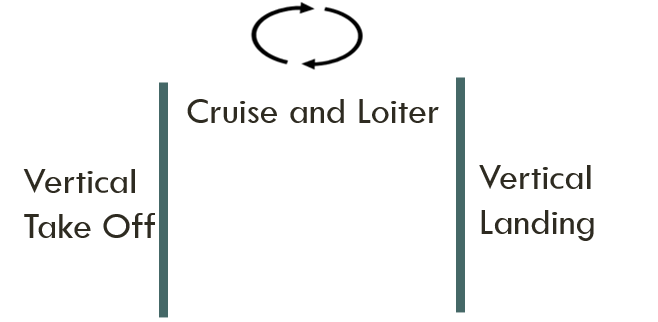
\includegraphics[width=7cm]{Simplified_mission.png}
    \begin{tikzpicture}[node distance = 2cm, xscale = 1,
						mainnode/.style = {inner sep = 0cm},
						mainpath/.style = {very thick,color=ist-gray},
						pathlabel/.style = {auto, black, font = \footnotesize, align = center}]
		\node (n1) at (0,0) [mainnode,				label = {180:1}] {};
		\node (n2)	[mainnode, above = of n1,   	label = {180:2}] {};
		\node (n3)	[mainnode, right = 4cm of n2,	label = {0:3}] {};
		\node (n4)	[mainnode, below = of n3,		label = {0:4}] {};
		\draw [mainpath] (n1.center) -- node [pathlabel] {Vertical \\ Take-Off} (n2.center) -- node [pathlabel,swap] {Cruise and Loiter} coordinate (magsearch_coor) (n3.center) -- node [pathlabel] {Vertical \\ Landing} (n4.center);
		\node (magsearch) [circle, pathlabel, above = 0.5cm of magsearch_coor, inner sep = 0cm] {Magnetic \\ Search};
		\draw[-{Stealth[]}] (magsearch) ++(110:1cm) arc[radius=1, start angle=110, end angle=250];
		\draw[-{Stealth[]}] (magsearch) ++(-70:1cm) arc[radius=1, start angle=-70, end angle=70];
	\end{tikzpicture}
    \caption{Simplified mission  profile}
    \label{Traca}
\end{figure}

It will be considered that the aircraft climbs to an altitude of cruise and loiter of $50$ meters, and a velocity of \SI{30}{\meter\per\second}. So if the aircraft can accomplish the mission under those circumstances, others will be covered (lower loiter speed). 

\chapter{Design Requirements} \label{chap:designreq}

To accomplish this mission, the aircraft should carry a magnetic anomaly detector, henceforth shortened to MAD, which will not be designed in this project. Other equipment (like avionics and antennas) would also be acquired in an \emph{off-the-shelf} format, and this design will only account for their weight, cost and volume.

\begin{description}
	\item[Weight] The airship should have a Maximum Take-Off Weight (MTOW) of \SI{35}{\kilo\gram} and it should be able to carry a payload of \SI{10}{\kilo\gram}.
	\item [Endurance] The UAV should be able to spend 5 hours in cruise flight.
	\item[Speed] The cruise speed of the aircraft should be \SI{30}{\meter\per\second} (\SI{58.3153}{\knot}).
	\item[Battery] It should have 5 to 10 minutes of battery backup.
	\item[Propulsion] The UAV should fly on hybrid-electric propulsion.
\end{description}
\pagebreak
\chapter{Market Overview}

The number of unmanned aerial vehicles flying in our airspace is now bigger than ever. The many advantages UAVs have over manned aircraft make them the most suitable for a growing variety of missions. In order to design a new UAV that fits the specific requirements of the mission previously described, it's important to start by researching existing competitors in the market that could provide useful data to the project.  In this section we will describe 5 existing UAVs with similar characteristics to those defined by our mission requirements, so we can have a better understanding of the possible design solutions that would work (or not) for this project. 

\section{Hybrid Quadrotor technology by Latitude Engineering}

This aircraft uses 4 rotors in order to achieve vertical takeoff and landing capabilities, and a back propeller for horizontal cruise flight.\cite{hquad} The back propeller is powered by a gas engine which provides long endurance fixed wing flight (15 hour endurance with the maximum payload of \SI{5.4}{\kilo\gram}). The four propellers for vertical flight are powered by electric lift motors that minimise the weight penalty of VTOL capabilities. This configuration brings the advantage of being more wind resistant than any other UAV configuration. \par
It can reach a cruise speed of \SI{40}{\knot}, and has a stall speed of \SI{30}{\knot}. Although this aircraft doesn’t fully accomplish our mission requirements, it presents several solutions that can be implemented in our UAV. 
\begin{figure}[ht]
    \centering
    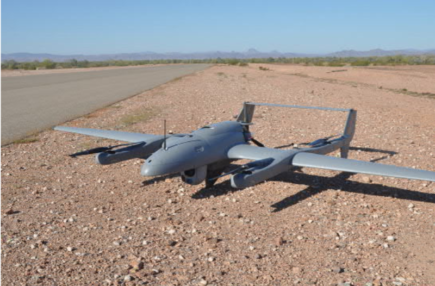
\includegraphics[width = 0.6\linewidth]{graphics/MarketOverview/HQ-90.png}
    \caption{HQ-90 by Latitude Engineering}
    \label{fig:hq90}
\end{figure}

\section{Reach by Alti}

With a fixed wing configuration, this UAV has five rotors that enable both VTOL capabilities and forward flight.\cite{reach} It is currently still in development, so the information available is limited. However, it is an upscaled version of Transition, a smaller UAV that is already available for purchase, and we can take valuable information from this pair of UAV’s that will be useful to our project. \par
The Reach aircraft has a payload capacity of \SI{7}{\kilo\gram} and endurance up to more than 20 hours. The wingspan is 6m, double the wingspan of Transition (3m). Transition’s maximum Take-Off Weight is \SI{16}{\kilo\gram}, so it's plausible to assume that Reach will have a MTOW close to the required for our project. Both aircrafts use hybrid propulsion. 
Although it is still in development, the Reach seems to accomplish most of our mission requirements. For that reason, our design was heavily influenced by this aircraft.

\begin{figure}[ht]
    \centering
    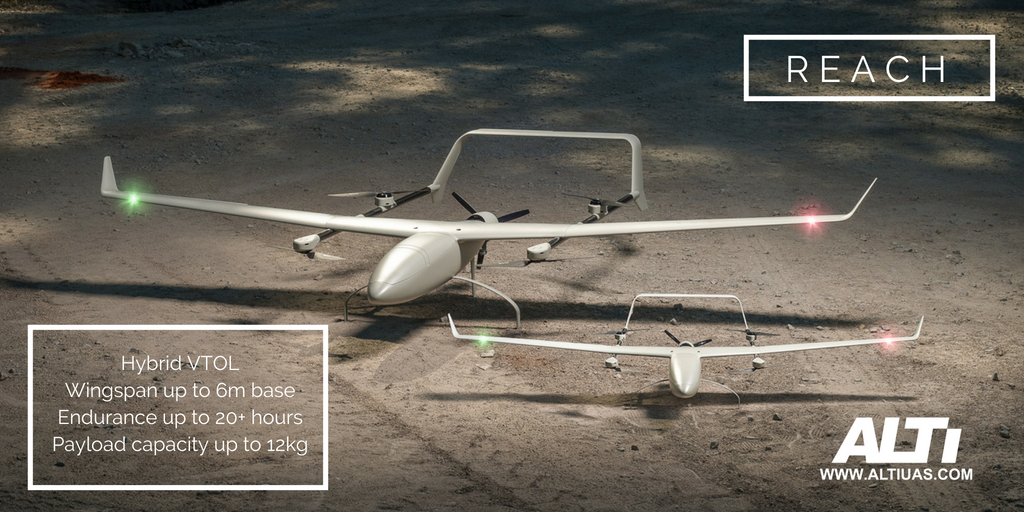
\includegraphics[width = 0.7\linewidth]{graphics/MarketOverview/reach.png}
    \caption{Reach and Transition by ALTI}
    \label{fig:reach}
\end{figure}


\section{Luna by EMT}

Luna is a lightweight UAV system in service since 2000 for mainly military applications.\cite{luna} Although this aircraft doesn't have VTOL capabilities, it can still give valuable information that might be useful to this project. It is launched with a bungee catapult and has the ability to glide without engine power. The glass fiber composite material it is made of provides long endurance (over 6 hours) and low acoustic, thermal and radar signatures. It has a MTOW of \SI{40}{\kilo\gram}, a wingspan of 4.17m 

\begin{figure}[ht]
    \centering
    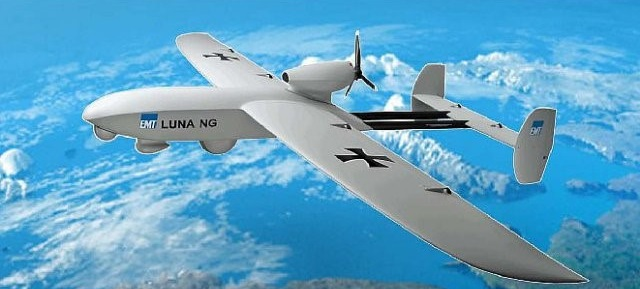
\includegraphics[width = 0.7\linewidth]{graphics/MarketOverview/Luna.jpg}
    \caption{Luna by EMT}
    \label{fig:luna}
\end{figure}

\section{Kari TR-60}


In order to explore the option to incorporate tilt mechanisms in our aircraft, we researched available UAVs that use tilt rotors to achieve vertical flight. TR-60 is an example of such aircrafts. It is manufactured by Korea Aerospace Research Institute (KARI) and reaches speeds of \SI{250}{\kilo\meter\per\hour}, a lot faster than our mission requirements.\cite{kari} It’s length and width are, respectively, 3 and 5m, and with a MTOW of \SI{210}{\kilo\gram}, it is also a lot heavier than our required weight, which is probably due to the tilt rotors. This suggests that tilt mechanisms aren’t appropriate for this particular mission, and this solution was therefore discarded in our project. 
\begin{figure}[ht]
    \centering
    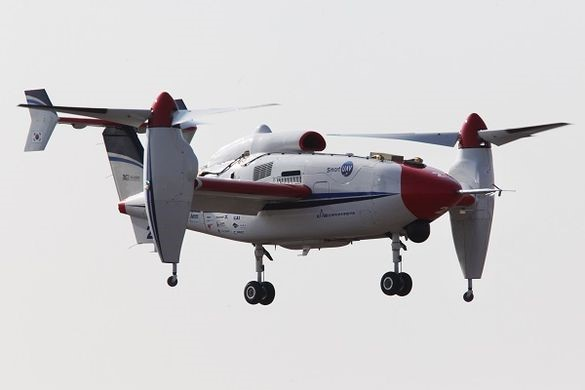
\includegraphics[width = 0.6\linewidth]{graphics/MarketOverview/KARI.jpg}
    \caption{Kari TR-60}
    \label{fig:kari}
\end{figure}

\section{PD1 by Height Technologies}

This hybrid powered fixed-wing UAV has an endurance of up to 10 hours \cite{pd1}. With a MTOW of \SI{40}{\kilo\gram} and a payload of \SI{10}{\kilo\gram}, it is intended to be equipped with a camera for military, industrial or mapping applications. It has a wingspan of \numrange[range-phrase = --]{5}{6} meters and uses 5 rotors. It is similar to Reach by Alti, the main difference being the inverted V-Tail which we incorporated in our project to avoid interference with the back rotor. Its modular design allows a quick and easy replacement of all airframe parts, which are secured with fastlink locks that require no tools to assemble or disassemble the UAV to maximise efficiency. 

\begin{figure}[ht]
    \centering
    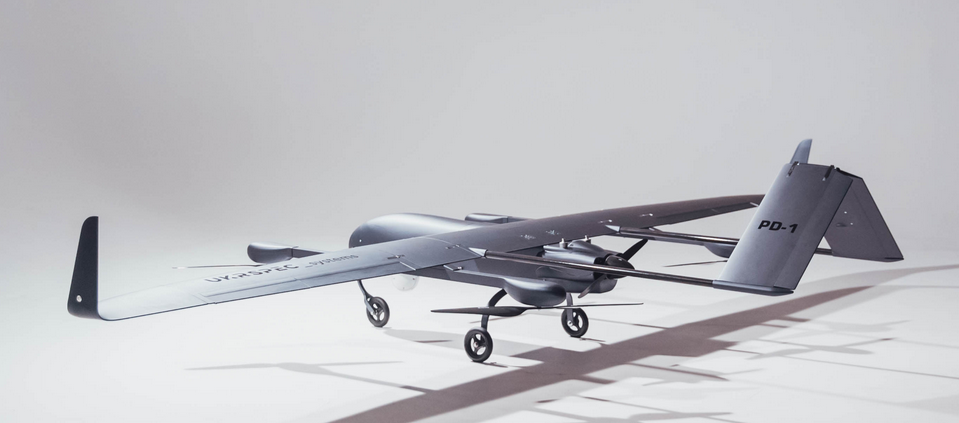
\includegraphics[width = 0.6\linewidth]{graphics/MarketOverview/pd1.png}
    \caption{PD1 by Height Technologies}
    \label{fig:pd1}
\end{figure}

\section{Comparison}
Table \ref{tab:uavs_comp} summarises the information available for all the aircrafts mentioned. 

%\begin{table}[ht]
%\begin{tabular}{|c|c|c|c|c|c|c|}
%\hline
%Aircraft              & \begin{tabular}[c]{@{}c@{}}MTOW\\   (Kg)\end{tabular} & \begin{tabular}[c]{@{}c@{}}Payload\\   (Kg)\end{tabular} & \begin{tabular}[c]{@{}c@{}}Endurance\\   (h)\end{tabular} & \begin{tabular}[c]{@{}c@{}}Cruise speed\\   (kts)\end{tabular} & \begin{tabular}[c]{@{}c@{}}Range\\   (NM)\end{tabular} & \begin{tabular}[c]{@{}c@{}}Service Ceiling\\   (ft)\end{tabular} \\ \hline
%\textbf{Requirements} & \textbf{35}                                           & \textbf{10}                                              & \textbf{5}                                                & \textbf{58.3153}                                               & \textbf{146}                                           & \textbf{-}                                                       \\ \hline
%HQ-90                 & 43                                                    & 5.4                                                      & 15                                                        & 40                                                             & 600                                                    & 14,000                                                           \\ \hline
%Reach                 & N/A                                                   & 7                                                        & +20                                                       & N/A                                                            & N/A                                                    & N/A                                                              \\ \hline
%Luna NG               & 40                                                    & N/A                                                      & 6                                                         & N/A                                                            & N/A                                                    & N/A                                                              \\ \hline
%TR-60                 & 210                                                   & 30                                                       & 5-6                                                       & 135                                                            & 108                                                    & 14,764                                                           \\ \hline
%PD1                   & 40                                                    & 10                                                       & 10                                                        & N/A                                                            & 539.96                                                 & 9842.5                                                           \\ \hline
%\end{tabular}
%    \caption{Comparison of different market-researched UAVs.}
%	\label{tab:uavs_comp}
%\end{table}

\begin{table}[ht]
    \centering
	\begin{tabular}{c c c c c c c}\toprule
		Aircraft
			& \makecell{MTOW\\(\si{\kilogram})}
			& \makecell{Payload\\(\si{\kilogram})}
			& \makecell{Endurance\\(\si{\hour})}
			& \makecell{Cruise\\Speed (\si{\knot})}
			& \makecell{Range\\($nm$)}
			& \makecell{Service\\Ceiling ($ft$)}	\\
		\midrule
		\textbf{Requirements}	& $\mathbf{35}$	& $\mathbf{10}$	& $\mathbf{5}$	& $\mathbf{58.3153}$	& $\mathbf{146}$	& \textbf{--}								\\
		HQ-90					& $43$			& $5.4$			& $15$			& $40$					& $600$				& \num[group-separator = \text{~}]{14000}	\\
		Reach					& n/a			& $7$			& $+20$			& n/a					& n/a				& n/a										\\
		Luna NG					& $40$			& n/a			& $6$			& n/a					& n/a				& n/a										\\
		TR-60					& $210$			& $30$			&
											\numrange[range-phrase = --]{5}{6}	& $135$					& $600$				& \num[group-separator = \text{~}]{14764}	\\
		PD1						& $40$			& $10$			& $10$			& n/a					& $539.96$			& \num[group-separator = \text{~}]{9842.5}	\\
		\bottomrule
	\end{tabular}
	\caption{Comparison of different market-researched UAVs.}
	\label{tab:uavs_comp}
\end{table}




\chapter{Conceptual Design}

In the configuration design process, different configuration options were evaluated based on the most important parameters (Aerodynamics, Stability and Control, Weight, Magnetic Interference). In order to choose the most suitable configuration for the intended UAV, a total of three configurations were considered.

\section{Considered Sample Configurations}

\subsection{Configuration 1}

The first configuration is sketched in figure \ref{fig:conf_1}. It represents a fixed-wing UAV with a relatively standard layout, with four rotors intended for use with VTOL placed to the side and fixed to the main structure.

\paragraph{Advantages of proposed architecture}
\begin{itemize}
	\item Rotors are capable of tilting to allow VTOL and horizontal flight; 
	\item Retraction of rotor blades (for drag reduction) enables efficient horizontal flight;
	\item Similar configuration already tested;
	\item Rotors are far away from the nose, reduced interference with the sensor.
\end{itemize} 

\paragraph{Disadvantages of proposed architecture}
\begin{itemize}
	\item Rotors exposed to the environment and vulnerable to damage from foreign objects;
	\item Rudder is in the wake of the tail rotor;
	\item Mechanical implementation of tilting rotors may be complex.
\end{itemize}

\begin{figure}[ht]
	\centering
	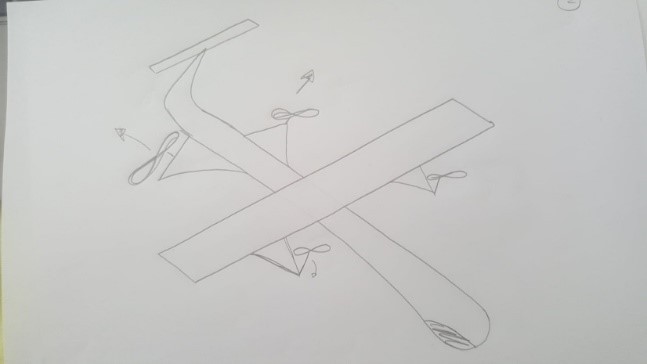
\includegraphics[width = 0.6\linewidth]{conf_1}
	\caption{Simplified sketch of configuration 1.}
	\label{fig:conf_1}
\end{figure}

\subsection{Configuration 2} 

\paragraph{Advantages of proposed architecture}
\begin{itemize}
	\item Rotors are capable of tilting to allow VTOL and horizontal flight; 
	\item Possibility of feathering;
	\item Less load applied to the wings.
\end{itemize}

\paragraph{Disadvantages of proposed architecture}
\begin{itemize}
	\item Rotors exposed to the environment and vulnerable to damage from foreign objects;
	\item Rudder is in the wake of the tail rotor;
	\item Mechanical implementation of tilting rotors may be complex;
	\item Difficult system of feathering;
	\item Fuselage might be overloaded by the rotors.
\end{itemize}

\begin{figure}[ht]
	\centering
	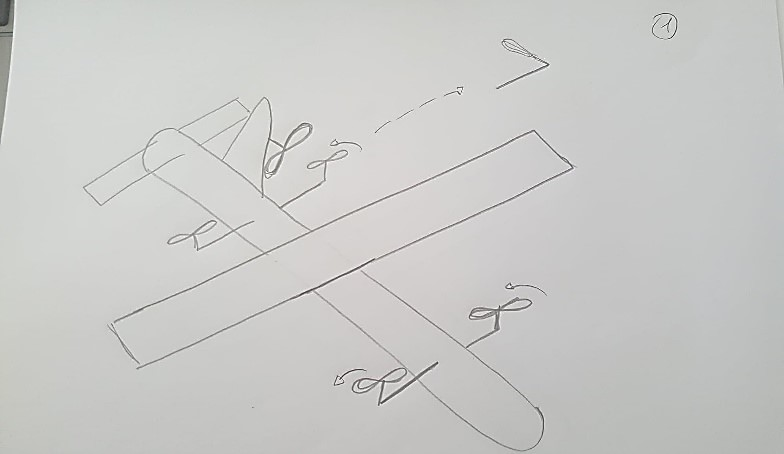
\includegraphics[width = 0.6\linewidth]{conf_2}
	\caption{Simplified sketch of configuration 2.}
	\label{fig:conf_2}
\end{figure}

\subsection{Configuration 3}

\paragraph{Advantages of proposed architecture}
\begin{itemize}
	\item Rotors are far away from the nose;
	\item Vertical take-off and efficient cruise possible;
	\item Rotor in the back is far away from the tail, which prevents aerodynamic interference.
\end{itemize}

\paragraph{Disadvantages of proposed architecture}
\begin{itemize}
	\item Fuselage is short, thus electric facilities cannot be stored very far away from the sensor;
	\item Rotors are not tilted to the front during cruise, thus aerodynamic drag might increase;
	\item Landing gear might not be strong enough to land forcefully.
\end{itemize}

\section{Analytic Hierarchy Process}

The AHP is a method to help in making complex decisions. First of all, the decision problem is divided into a hierarchy of subproblems, each of which can be analyzed independently. Based on this division, evaluations are made to the most important parameters of each subproblem and converted into numerical classifications according to table \ref{tab:grades_scale}. It is assigned to each parameter and subproblem a weight that represents its importance in the set. In the end, the option chosen is the one that globally collects a better rating.

\begin{table}[ht]
	\centering
	\begin{tabular}{c|c}\toprule
		Grade	& Definition			\\
		\midrule
		1		& Very poor performance	\\
		2		& Poor performance		\\
		3		& Averange performance	\\
		4		& Good performance		\\
		5		& Very good performance	\\
		\bottomrule
	\end{tabular}
	\caption{The scale of grades.}
	\label{tab:grades_scale}
\end{table}

\begin{table}[ht]
	\centering
	\begin{tabular}{c|C C C}\toprule
		\textbf{Configuration}			& 1		& 2		& 3			\\
		\midrule
		\textbf{Aerodynamics}			& 3.7	& 2.9	& 3.9		\\
		\midrule
		Performance						& 4		& 4		& 4			\\
		Induced drag					& 3		& 3		& 4			\\
		Interference drag				& 4		& 2		& 4			\\
		Tail propeller interaction		& 3		& 3		& 3			\\
		\midrule
		\textbf{Stability and control}	& 3.7	& 3.8	& 4			\\
		\midrule
		Center of gravity position		& 2		& 4		& 3			\\
		Aircraft stability				& 5		& 4		& 5			\\
		Maneuverability					& 3		& 3		& 3			\\
		\midrule
		\textbf{Weight}					& 2.7	& 3.7	& 4			\\
		\midrule
		Payload							& 2		& 3		& 4			\\
		Structures						& 3		& 4		& 4			\\
		\midrule
		\textbf{Magnetic interference}	& 3.7	& 3.4	& 3.7		\\
		\midrule
		Positioning of avionics			& 4		& 4		& 4			\\
		Position of rotors				& 3		& 2		& 3			\\ 
		Position of battery and electric generator	& 4	& 4	& 4		\\
		\midrule
		\textbf{Total}					& 3.5	& 3.3	& 3.8		\\
		\bottomrule
	\end{tabular}
	\caption{Configuration analysis with the AHP method.}
	\label{tab:ahp_evaluations}
\end{table}

\chapter{Initial Weight Estimation and Design Point} \label{chap:designpoint}

The first step in an aircraft project is to find and analyse the mission profile in order to obtain some numbers that can be the start of the conceptual design. As mentioned before, a simplified version of the mission profile will be used. 

The provided MATLAB code was the start point. Some assumptions were made: 
\begin{itemize}
    \item $C_{d_0} = 0.03$. The normal range of this value goes from $0.01$ to $0.02$, but as the VTOL rotors and its respective structure will cause a significant increase in the drag, $0.03$ was the chosen value for this variable;
    \item Maximum power of \SI{10}{\kilo\watt};
    \item Power factor of $1.5$;
    \item Thrust-to-weight ratio of $1.3$;
    \item Endurance of $5$ hours, with a reserve of $10$ minutes;
    \item Hover time of $3$ minutes, assuming $1.5$ minutes when taking off and landing;
    \item Cruise speed of \SI{30}{\meter\per\second};
    \item Energy specific density for the batteries of \SI{165}{\watt\hour\per\kilogram}, with a $10$ percent reserve;
    \item power to weight ratio of the electric motors of \SI{4.5}{\kilo\watt\per\kilogram}
    \item Specific fuel consumption regarding the combustion engine of $0.6\,Kg/Hp\cdot h$ and a power to weight ratio of \SI{2.38}{\kilo\watt\per\kilogram}
    \item Concerning the propeller blades, it was assumed a solidity of $0.1$, a $C_{d_0}$ of $0.01$, an induced power coefficient of $1.1$ (typical values range from $1.1$ to $1.15$), and a tip mach of $0.6$ due to noise interference;
    \item Avionics, electronics weight of $15\%$ of the total empty weight;
    \item Structural weight of $24\%$ of the total aircraft weight;
    \item Disk loading of \SI{35}{\kilogram\per\meter\squared};
    \item $\eta_p=0.4$ which is a typical value for a pusher engine configuration.
\end{itemize}
 
Inside the MATLAB code cycle, two new formulas that are more suitable for small aircraft analysis were introduced.
\begin{gather*}
    \frac{L}{D}=0.94\times \frac{1}{2\times \sqrt{C_{d_0} \times K}}
\end{gather*}
where
\begin{gather*}
    K=\frac{1}{\pi\cdot AR\cdot e}
\end{gather*}
and a aspect ratio of $10$ was assumed.
\begin{gather*}
    P_c=\frac{MTOW \times V_c}{L/D}\cdot\frac{1}{1000}
\end{gather*}
$V_c$ being the cruise velocity. 

What comes out of the cycle are the following results.

\begin{table}[ht]
    \centering
    \begin{tabular}{l c}\toprule
         & \textbf{Results} \\
        \midrule
        MTOW                        & \SI{31.7469}{\kilogram} \\
        Empty weight                & \SI{12.7208}{\kilogram} \\
        Payload                     & \SI{9.6461}{\kilogram} \\
        Structural mass             & \SI{7.6193}{\kilogram} \\
        Propulsive system           & \SI{3.1934}{\kilogram} \\
        Fuel                        & \SI{7.1354}{\kilogram} \\
        Batteries                   & \SI{2.2447}{\kilogram} \\
        VTOL rotor radius           & \SI{0.3092}{\meter} \\
        Installed power for cruise  & \SI{1.7164}{\kilo\watt} \\
        \bottomrule
    \end{tabular}
    \caption{Weight results for the MATLAB code cycle.}
    \label{tab:matlabcycle}
\end{table}
As shown is the previous table, the MTOW is below the required \SI{35}{\kilogram}, and the payload is close to the \SI{10}{\kilogram} required weight. Once again, these results are viable for an aircraft in cruise conditions, that does not have to climb, descent or make any manoeuvres. As a safety margin, a new design point was computed to address all these situations. The following assumptions were made
\begin{itemize}
    \item Stall speed of \SI{25}{\meter\per\second}, which is very close to the cruise speed, but in order so save weight am make this aircraft as cruise focused as possible, these was the chosen speed.
    \begin{itemize}
        \item Notice that as this is a VTOL aircraft, the transition phase can be assisted by the VTOL engines until it reaches the cruise velocity;
    \end{itemize}
    \item Maximum lift coefficient of $1.2$;
    \item A climb angle of $3$ degrees, which can provide the aircraft with some manoeuvrability capabilities.
\end{itemize}

For the design point computation, the chosen requirements were the range, the endurance, the climb angle and the stall speed. The equations for these restrictions were adapted from \citetitle{corke} \cite{corke}, and can be found in equations \ref{eq:restrictions}. Equation \ref{eq:cruise_speed} corresponds to the cruise speed restriction, equation \ref{eq:climb_angle} is the climb angle, \ref{eq:stall_speed} for the stall speed, \ref{eq:range} for range, and \ref{eq:endurance} for endurance.
\begin{subequations}\label{eq:restrictions}
    \begin{align}
        \frac{P}{W} &\geq \frac{1}{\eta_p}\left(\frac{\rho V^3C_{D_0}}{2\frac{W}{S}} + \frac{2k}{\rho V}\frac{W}{S}\right) \label{eq:cruise_speed} \\
        \frac{P}{W} &\geq \frac{V}{\eta_p}\left(G + \frac{\rho V^2 C_{D_0}}{2\frac{W}{W}} + \frac{2k}{\rho V^2}\frac{W}{S}\right) \label{eq:climb_angle} \\
        \frac{W}{S} &\leq \frac{\rho V_S^2}{2}\left(C_L\right)_{\text{max}} \label{eq:stall_speed} \\
        \frac{W}{S} &= \frac{\rho V_S^2}{2}\sqrt{\frac{C_{D_0}}{k}} \label{eq:range} \\
        \frac{W}{S} &= \frac{\rho V_S^2}{2}\sqrt{\frac{3C_{D_0}}{k}} \label{eq:endurance}
    \end{align}
\end{subequations}

%\begin{figure}[ht]
%	\centering
%	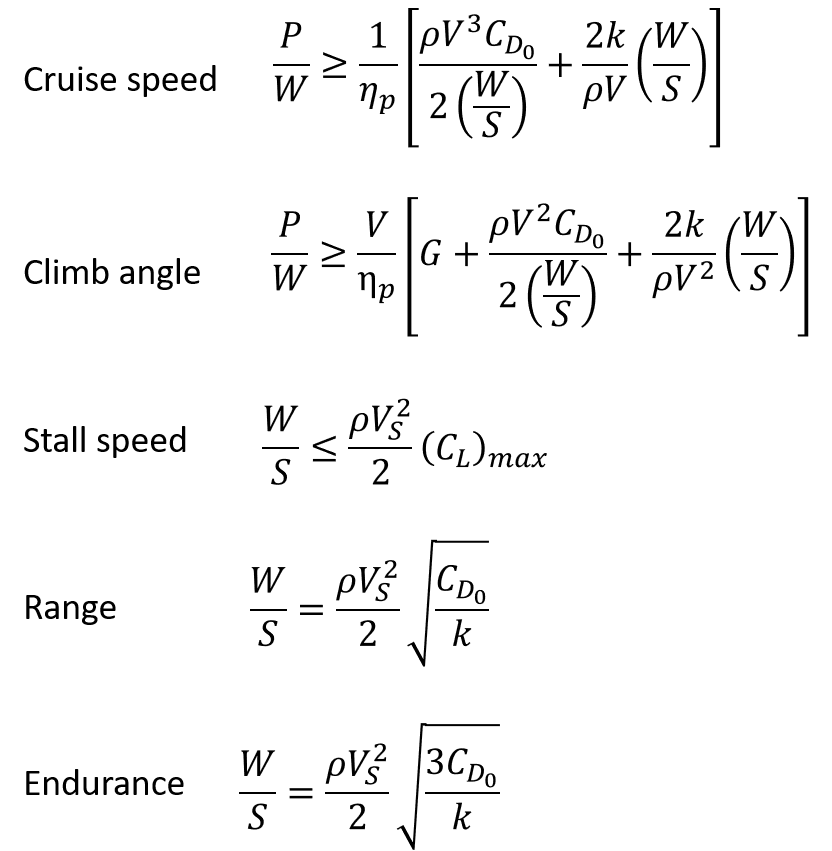
\includegraphics[width = 0.4\linewidth]{Design_point_equations.png}
%	\caption{Restrictions of the design point.}
%	\label{fig:dp_restrictions}
%\end{figure}

The result is the design space found in figure \ref{fig:dp_space_tikz}.

%\begin{figure}[ht]
%	\centering
%	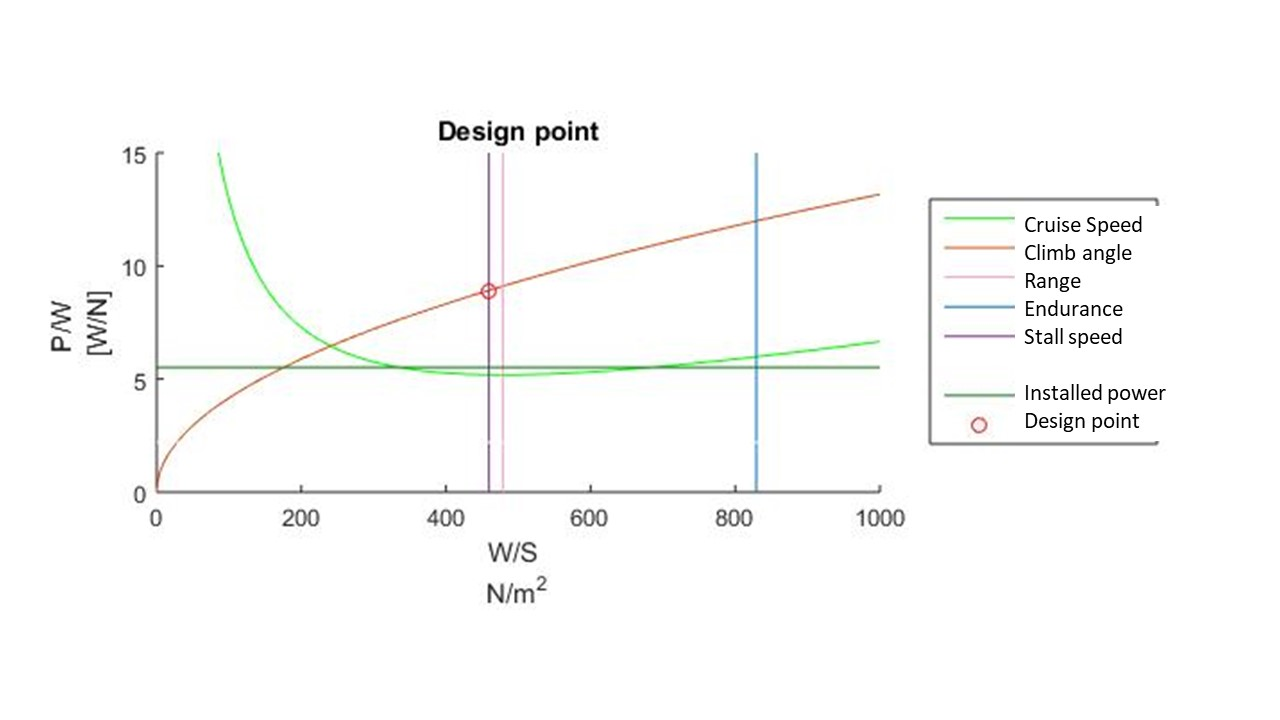
\includegraphics[width = \linewidth, trim = {8mm 4cm 3cm 3cm}, clip]{Design_point.jpg}
%	\caption{Design point space}
%	\label{fig:dp_space}
%\end{figure}

\begin{figure}[ht]
    \centering
    \begin{tikzpicture}
    \begin{axis}
            [width = 0.7\linewidth,
            xmin = 0, xmax = 1000,
            ymin = 0, ymax = 15,
            xlabel = {$\frac{W}{S}$},
            ylabel = {$\frac{P}{W}$},
            legend pos = outer north east,
            cycle list = {red,blue,cyan,teal,orange,purple,violet,brown,darkgray,magenta},]
        \addplot table [col sep = comma, x index = {0}, y index = {1}] {designpoint.csv};
        \addplot table [col sep = comma, x index = {0}, y index = {2}] {designpoint.csv};
        \addplot coordinates {(478.662,-1) (478.662,16)};
        \addplot coordinates {(829.0673,-1) (829.0673,16)};
        \addplot coordinates {(459.375,-1) (459.375,16)};
        %\addplot coordinates {(-1,2.20528) (1001,2.20528)};
        \addplot coordinates {(-1,5.5132) (1001,5.5132)};
        \addplot [mark = o, color = red] coordinates {(458.875,8.91737)};
        %\legend{Cruise Speed, Climb Angle, Range, Endurance, Stall Speed, Cruise Power, Installed Power, Design Point}
        \legend{Cruise Speed, Climb Angle, Range, Endurance, Stall Speed, Installed Power, Design Point}
    \end{axis}
\end{tikzpicture}
    \caption{Design point calculation.}
    \label{fig:dp_space_tikz}
\end{figure}

In order to minimise the aircraft required power and to minimise the needed wing area, the design point chosen is the marked in the figure with a red circle, and has the following ratios: 

\begin{gather*}
    \frac{P}{W} = 8.9174\,W/N \\
    \frac{W}{S} = 458.8750\,N/m^2
\end{gather*}

Recovering the MTOW value of \SI{31.7469}{\kilogram}, the design point ratios provide us with the wing area of \SI{0.6785}{\meter\squared} and a rear engine \SI{2.7763}{\kilo\watt} respectively. 

It is important to notice the difference between the line regarding the installed power for cruise (calculated with the formula inside the MATLAB file cycle) and the final rear engine power. It is clear that the line of the cruise speed restriction and the installed power converges with the increasing W/S. So, the difference between the two values of power is caused by the assign capability for the aircraft to climb at a angle of 3 degrees and to overcome the drag cause by a wing which is capable to present a stall velocity of \SI{25}{\meter\per\second}.

The design point for the vertical climb and landing is represented in the graph found in figure \ref{fig:design_point_restrictions}. Again, a disk loading of \SI{35}{\kilogram\per\meter\squared} was assumed so the obtained design point lies on the interception of the two shown curves. 

\begin{figure}[ht]
	\centering
	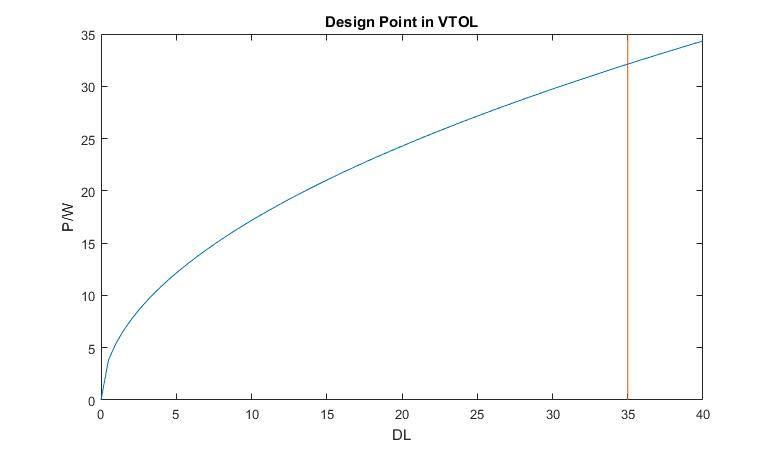
\includegraphics[width = 0.6\linewidth]{Design_point_vtol.jpg}
	\caption{Restrictions of the design point.}
	\label{fig:design_point_restrictions}
\end{figure}

\begin{equation}
    \frac{P_{máx}}{W} \ge \frac{PF}{FoM}\times \frac{T}{W} \sqrt{\frac{DL\times g}{2\rho}}
\end{equation}

Using the values obtained from the MATLAB code, the rotors figure of merit ($FoM$) is equal to $0.7186$, the power factor was assumed to be equal to $1.5$, and the thrust to weight ratio to $1.3$. Thus, the vertical manoeuvres design point is characterised by the following power to weight ratio:
\begin{subequations}
    \begin{gather}
        \frac{P}{W} = \SI{32}{\watt\per\newton}
    \end{gather}
    or
    \begin{gather}
        \frac{P}{W} = \SI{3.1867}{\kilo\watt\per\kilogram}
    \end{gather}
\end{subequations}

\begin{figure}[ht]
	\centering
	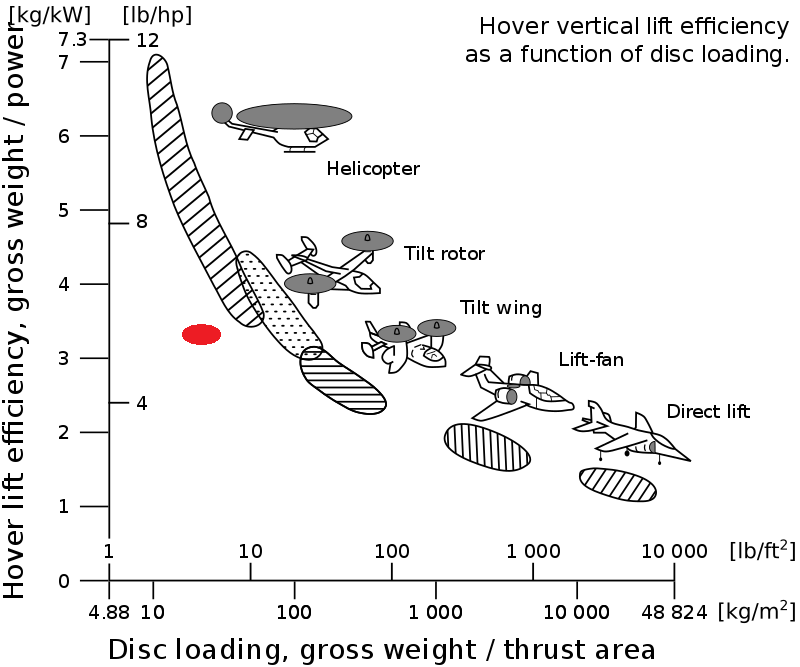
\includegraphics[width = 0.6\linewidth]{graphics/Disk_loading_different_aircraft.png}
	\caption{Typical design points}
	\label{fig:typical_vertical_design_point}
\end{figure}

Analysing the figure \ref{fig:typical_vertical_design_point} is clearly noticeable that the design point for the projected aircraft lies very close to the typical range of design points characteristic to the vertical take off and landing aircraft.

However, in this project, a different approach for the computation of the electric motors power and rotor radius was made, explained in chapter \ref{chap:power}.

\chapter{Wing Design}\label{chap:wingDesign}
\section{Wing Planform}
The next step in this project was to determine the wing dimensions. In the previous chapter we assumed an aspect ratio AR of 10 and obtained a wing area W of $0,6785m^2$. From this data, we used the formula \ref{eq:wingspan} to determine the wingspan b of our aircraft. 
\begin{equation}\label{eq:wingspan}
    AR=\frac{b^2}{S}
\end{equation}
\begin{center}
    $\Rightarrow b=2,605m$
\end{center}

As described in Chapter \ref{chap:missionprofile}, our mission requires a cruise speed of \SI{30}{\meter\per\second} at an altitude of \SI{50}{\meter} ($164\,ft$). \par
The formula \ref{eq:mach} can be used to determine the Mach number at cruise. 
\begin{equation}\label{eq:mach}
    V=[1036-0.0034\cdot (h-20000)] \cdot M
\end{equation}
\begin{center}
    $\Rightarrow M=0.089$
\end{center}

 Figures 4.12, 4.10 and 4.05 from Corke's Textbook (shown in Figure \ref{fig:corke}) give us the leading edge sweep angle (which we can consider equal to the sweep angle of the quarter-chord line), the taper ratio and the maximum thickness-to-chord ratio. 
 
 \begin{figure}[ht]
     \centering
     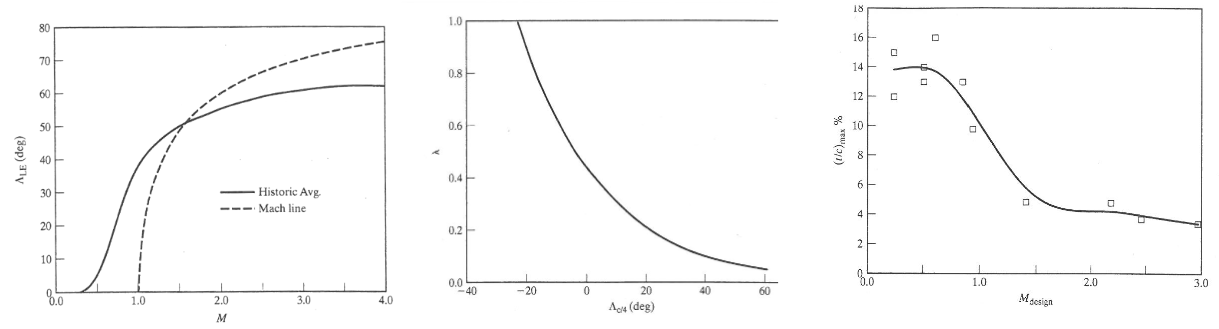
\includegraphics[width=\textwidth]{graphics/WingDesign/corke.png}
     \caption{Figures 4.12 (left), 4.10 (center) and 4.05 (right) from \citetitle{corke} \cite{corke}.}% Corke's Textbook}
     \label{fig:corke}
 \end{figure}
 
 Therefore, we have a sweep angle of $\Lambda_{LE} =0$, a taper ratio of $\lambda=0.43$ and a maximum thickness-to-chord ratio of $(\frac{t}{c})_{max}=0.1375$. We can use this data and the formulas \ref{eq:croot} and \ref{eq:ctip} to determine the chord at the root and at the tip of the wing, respectively. 

\begin{equation}\label{eq:croot}
    c_{root}=\frac{2b}{AR(1+\lambda)}
\end{equation}
\begin{center}
    $\Rightarrow c_{root} \approx 0.364m  $
\end{center} \newpage
\begin{equation}\label{eq:ctip}
    \lambda = \frac{c_{tip}}{c_{root}}
\end{equation}
\begin{center}
    $\Rightarrow c_{tip} \approx 0.157m  $
\end{center}

The obtained wing dimensions are represented in Figure \ref{fig:planform}.

\begin{figure}[ht]
    \centering
    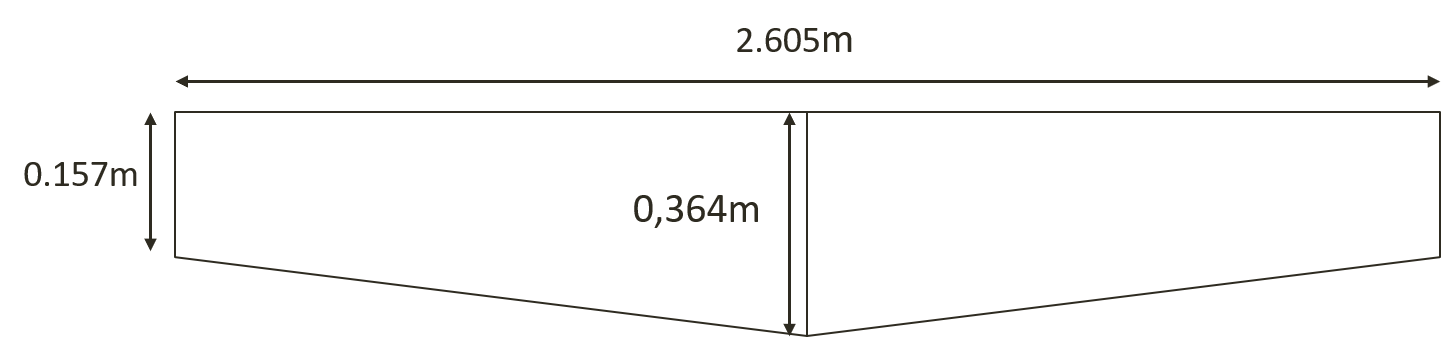
\includegraphics[width=\textwidth]{graphics/WingDesign/planform.png}
    \caption{Wing planform}
    \label{fig:planform}
\end{figure}

\section{Airfoil Selection}
The airfoil was selected according to the maximum thickness to chord ratio, as well as the average Reynolds number, determined by the formula \ref{eq:reynolds}, where x is the mean chord and $\nu$ is the kinematic viscosity, given by \ref{eq:viscosity}, with dynamic viscosity of $\mu= 1.789\times 10^{-5}$ and air density of $\rho=1,225$ at cruise altitude.
\begin{equation} \label{eq:reynolds}
    Re_x=\frac{V\cos{\Lambda_{LE}}x}{\nu}
\end{equation}
\begin{center}
    $\Rightarrow Re_x \approx 563408 $
\end{center} \par
\begin{equation} \label{eq:viscosity}
    \nu = \frac{\mu}{\rho}
\end{equation}
\begin{center}
    $\Rightarrow \nu \approx 1.46\times 10^{-5} $
\end{center}

Among the options available at Airfoil Tools \cite{e210} we selected Eppler E210 low Reynolds number airfoil, shown in figure \ref{fig:e210_profile}.

%\begin{figure}[ht]
%    \centering
%    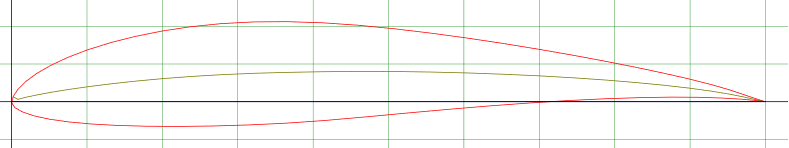
\includegraphics[width=0.8\textwidth]{graphics/WingDesign/airfoil.png}
%    \caption{Eppler E210 low Reynolds number airfoil}
%    \label{fig:airfoil}
%\end{figure}
\begin{figure}[ht]
    \centering
    \begin{tikzpicture}
        \begin{axis}[ymin = -0.12, ymax = 0.18, grid = both, width = \linewidth, height = 5cm]
			\addplot [mark=none,color=red] table [col sep = space, x index = {0}, y index = {1}] {e210.dat};
        \end{axis}
    \end{tikzpicture}
    \caption{Eppler E210 low Reynolds number airfoil \cite{e210}.}
    \label{fig:e210_profile}
\end{figure}

This airfoil seemed the most adequate to our aircraft, not only because it maximises the $Cl/Cd$ ratio (figure \ref{fig:airfoilgraphs1}, left) but also because the lift coefficient doesn’t drop abruptly at stall (figure \ref{fig:airfoilgraphs1}, right).

Further data regarding the airfoil derivatives can be found in figure \ref{fig:e210_data} from page \pageref{fig:e210_data}.

\begin{figure}[ht]
    \centering
    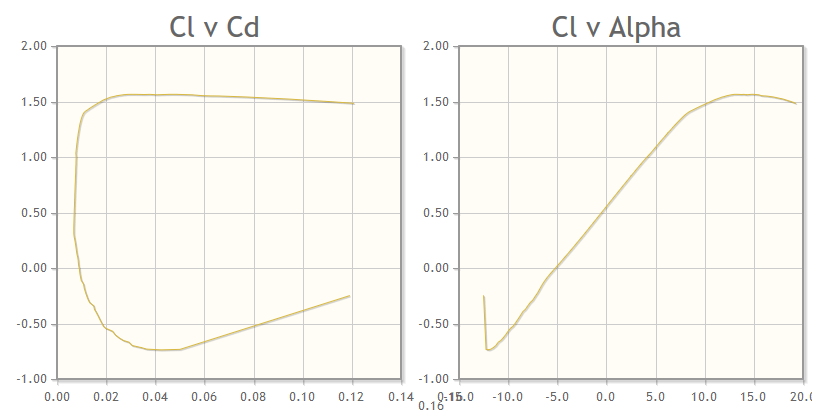
\includegraphics[width=\textwidth]{graphics/WingDesign/airfoilgraphs1.png}
    \caption{$C_L$ as a function of $C_D$ (left) and $C_L$ as a function of $\alpha$ (right)}
    \label{fig:airfoilgraphs1}
\end{figure}


\begin{figure}[ht]
    \centering
    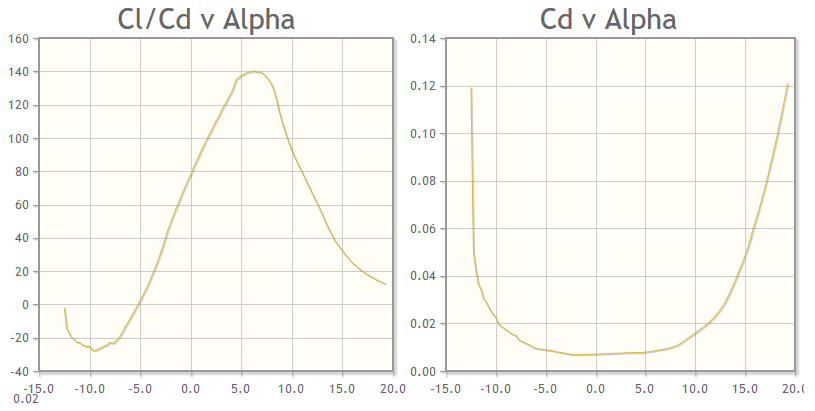
\includegraphics[width=\textwidth]{graphics/WingDesign/airfoilgraphs2.png}
    \caption{$\frac{C_L}{C_D}$ as a function of $\alpha$ (left) and $C_D$ as a function of $\alpha$ (right)}
    \label{fig:airfoilgraphs2}
\end{figure}


\begin{figure}[ht]
    \centering
    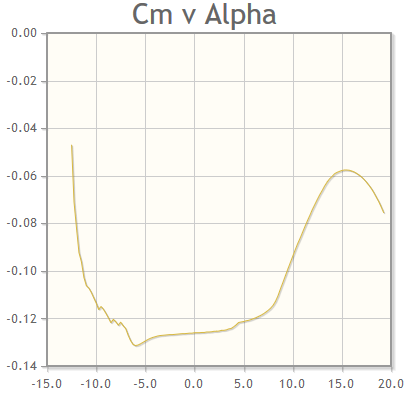
\includegraphics[width=0.5\textwidth]{graphics/WingDesign/airfoilgraphs3.png}
    \caption{$C_m$ as a function of $\alpha$}
    \label{fig:airfoilgraphs3}
\end{figure}


\chapter{Rotor Design} \label{chap:rotordesign}
In order to give our aircraft VTOL capabilities, it is necessary to equip it with a set of rotors capable of producing enough thrust to raise the total weight of the vehicle. In this section we will present the aspects related to the design of the rotors necessary for vertical take-off and landing, including the method used to obtain the value of their radius. All calculations covered in this chapter can be found in the MATLAB file. These calculations were performed in the iterative process also used to determine the mass of the batteries and the initial MTOW. \par
As described in Chapter \ref{chap:designpoint} some values were assumed for the initial calculation of the design point. The relevant ones for determining the rotors’ radius are the following:
\begin{itemize}
    \item Maximum installed power of 10kW;
    \item Power factor of 1.5;
    \item Thrust-to-weight ratio of 1.3;
    \item Concerning the propeller blades, it was assumed a solidity (s) of 0.1, a Cd0 of 0.01, an Induced Power Coefficient ($k_i$) of 1.1 and a Tip Mach of 0.6 due to noise interference;
    \item Disk loading of \SI{35}{\kilogram\per\meter\squared};
    \item Unducted rotor configuration.
\end{itemize}
Through these assumptions and using the equation \ref{eq:powertohover} (which is valid because the rotors are unducted), we obtain a Power to Hover of $6.67kW$. This equation is included in the MATLAB cycle, but since Maximum Installed Power and Power Factor are constants then the Power to Hover is independent of the iteration.

%\begin{equation} \label{eq:powertohover}
%    \text{Power to Hover}=  \frac{\text{Maximum Installed Power}}{\text{Power Factor}}
%\end{equation}
%\begin{center}
%    Power to Hover = $\frac{10 kW}{1.5}=6.67kW$
%\end{center}
\begin{gather}\label{eq:powertohover}
    \begin{aligned}
        \text{Power to Hover} &= \frac{\text{Maximum Installed Power}}{\text{Power Factor}} \\
        &= \frac{\SI{10}{\kilo\watt}}{1.5} = \SI{6.67}{\kilo\watt}
    \end{aligned}
\end{gather}

The equations \ref{eq:thrusttohover}, \ref{eq:rotorradius}, \ref{eq:ct} and \ref{eq:figmerit} were also included in the iterative cycle of the MATLAB file. The equation \ref{eq:thrusttohover} allows us to obtain the Thrust to Hover, i.e. the value we need to get when we sum the thrust contribution of all the rotors, in order to perform vertical take-offs and landings.  \par
The equation \ref{eq:rotorradius} computes the radius of each of the propellers’ blades. Finally, the equation \ref{eq:ct} allows us to calculate the blade mean lift coefficient ($C_t$) which is a necessary parameter to determine the Figure of Merit of the Rotors by the equation \ref{eq:figmerit}.

\begin{equation} \label{eq:thrusttohover}
    \text{Thrust to Hover}=\text{Thrust to Weight Ratio}\times MTOW
\end{equation}

\begin{equation} \label{eq:rotorradius}
    \text{Rotor Radius}=\sqrt{\frac{\text{Thrust to Hover}}{g\times\pi\times \text{Number of Rotors} \times \text{Disk Loading}}}
\end{equation}

\begin{equation} \label{eq:ct}
    C_t=\frac{\text{Disk Loading}\times g}{1.1\times\rho\times V_{tip}}
\end{equation}

\begin{equation} \label{eq:figmerit}
    \text{Figure of Merit}=\frac{1}{k_i+\frac{\frac{3}{4}C_{D_0}}{6\times k_i\times\sqrt{\frac{C_t}{s}}}}
\end{equation}


The number of rotors to be used was based on the chosen UAV configuration. In the chapter dedicated to Conceptual Design we concluded that the most advantageous configuration for the design requirements and the nature of the mission (magnetic anomaly detection) would be a configuration similar to Alti Reach. Therefore, 4 rotors will be incorporated in our UAV to guarantee VTOL capabilities without significantly disturbing the magnetic sensor.

\begin{equation*}
    \text{Number of Rotors} = 4
\end{equation*}

Assuming the use of 4 rotors and through the equations \ref{eq:thrusttohover},\ref{eq:rotorradius}, \ref{eq:ct} and \ref{eq:figmerit} listed above, we obtained the following values in the final iteration of the cycle performed in the MATLAB:
\begin{equation*}
    \text{Thrust to Hover}=404.7N
\end{equation*}
\begin{equation*}
    \text{Rotor Radius}=0.3092m= 30.92cm
\end{equation*}
\begin{equation*}
    \text{Figure of Merit}=0.7196
\end{equation*}

These parameters characterise the rotors of our aircraft and when we look for commercially available solutions we will have to satisfy these values. \par
Regarding the number of blades, since we must to keep in mind the environmental goals of achieving low pollutant and noise emissions, we will select the most efficient option, which is to use the traditional 2 blades instead of 3. The use of 2 blades is also advantageous because it favours the configuration of the PID controllers.

\begin{equation*}
    \text{Number of Blades}=2
\end{equation*}

Finally, in relation to the blades themselves, since the UAV that is being projected is small (MTOW of 31kg) it is not necessary to design custom blades: we can use one of several solutions available in the market, such as the ones of the company KDE Direct. In chapter \ref{chap:prop} we will present our choice of commercial rotors and commercial propeller blades. 

\begin{figure}[ht]
    \centering
    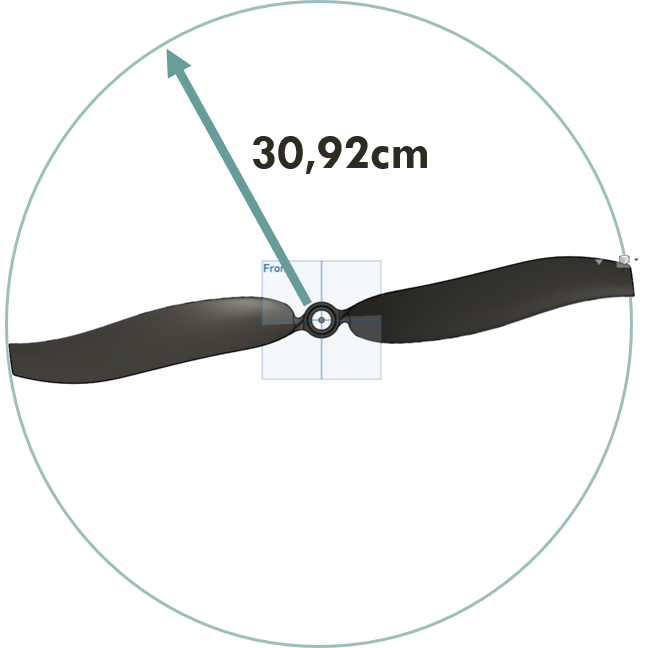
\includegraphics[width=0.2\textwidth]{graphics/WingDesign/rotordesign.png}
    \caption{Rotor Design}
    \label{fig:rotordesign}
\end{figure}




\chapter{Battery Weight for Hover} \label{chap:bathover}
In order to store the required power for the Vertical Take-Off and Landing steps it’s necessary to have batteries. The batteries store the energy for the hover stages and give the rotors proper voltages and currents to generate a combined thrust equal to or greater than the projected Thrust-to-Weight ratio. The mass of the batteries must also be considered for the determination of the MTOW. Therefore, we included the determination of the batteries’ mass in the iterative process used to obtain the MTOW.\par
The important values for the determination of the batteries’ mass and are the following (the energy specific density for the batteries was attributed after a market analysis):
\begin{itemize}
    \item Maximum installed power of 10kW;
    \item Power factor of 1.5;
    \item Hover time of 3 minutes = 180 seconds, assuming 1.5 minutes when taking off and landing;
    \item $E_{\text{bat}}$ = Energy specific density for the batteries of $165Wh kg^{-1}$, with a 10 percent reserve;
\end{itemize}
Through these assumptions and using the equation \ref{eq:powertohover} we obtain a Power to Hover of $6.67kW$.

%\begin{equation}\label{eq:powetohover}
%    \text{Power to Hover}=\frac{\text{Maximum Installed Power}}{\text{Power Factor}}
%\end{equation}
%\begin{center}
%    Power to Hover=$\frac{10kW}{1.5}=6.67kW$
%\end{center}

\begin{gather}\label{eq:powetohover}
    \begin{aligned}
        \text{Power to Hover} &= \frac{\text{Maximum Installed Power}}{\text{Power Factor}} \\
        &= \frac{\SI{10}{\kilo\watt}}{1.5} = \SI{6.67}{\kilo\watt}
    \end{aligned}
\end{gather}

Once obtained the Power to Hover, we use the energy specific density of the batteries and the total hover time to determine the batteries’ final weight. The equation \ref{eq:wbatteries} establishes the relationships between these variables and through its use we obtain a total weight of batteries of $2,447 kg$.

\begin{equation}\label{eq:wbatteries}
    W_{\text{batteries}}=\frac{\text{Power to Hover} \times \text{Hover Time} }{E_{\text{bat}}\ (1-reserve)}
\end{equation}

\begin{equation*}
    W_{\text{batteries}}=\frac{6.67\times{10}^3\times180}{165\times3600(1-0.1)}=2.447 kg
\end{equation*}

In chapter \ref{chap:power} we will choose a commercial battery that meets the characteristics expressed in this chapter. The total storage capacity of this battery must be in accordance with the equation \ref{eq:batstorcapacity}.

\begin{equation} \label{eq:batstorcapacity}
    \text{Battery Storage Capacity } [Wh]=W_{\text{battery}}[kg]\times E_{\text{bat}}\ [Wh/Kg] 
\end{equation}
\begin{equation*}
    \text{Battery Storage Capacity } [Wh]= 165\times2.2447=403.755 \ Wh
\end{equation*}
\begin{equation*}
    \text{Battery Storage Capacity } [Wh]=\left[VAh\right]=403.755 \ VAh
\end{equation*}




\chapter{Fuselage Design}

The fuselage has to fulfil several requirements, i.e. it has to accommodate the whole equipment inside, namely the sensor, the battery, the fuel tank, the cruise engine, the avionics and additional payload. On the other hand the fuselage has to be designed in a way that the drag is minimised.

\section{Internal layout}

To receive an initial design of the fuselage, the positioning of the contained components is considered. The positioning of the components inside the fuselage are displayed in figure \ref{fig:fuseInt2}.

\begin{figure}[ht]
	\centering
	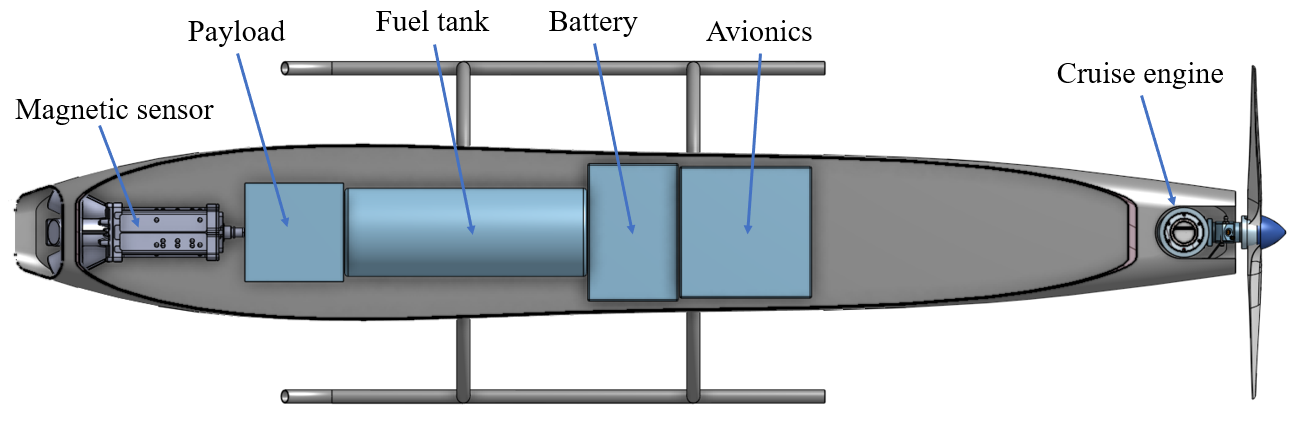
\includegraphics[width = 1\linewidth]{fuselageInternal2.png}
	\caption{Positioning of the components inside the fuselage.}
	\label{fig:fuseInt2}
\end{figure}

The magnetic sensor will be positioned in the nose of the fuselage. The most important reason for this is the influence of the other components on the measurement of the magnetic sensor. The further other components are away from the sensor, the less effect they have on the measurement.

Behind the sensor will the payload be positioned. The payload is assumed to have no effect on the magnetic measurement and brings a load of $8.5\ \mathrm{kg}$ to the front in order to keep the static margin high.

The positioning of the fuel tank behind the payload is close to the centre of gravity. This brings the positive effect that the centre of gravity does not dramatically change during cruise as fuel is burned. Since the fuel tank is made of carbon fibre epoxy it has no influence on the magnetic measurement either.

One of the closest components to the magnetic sensor, which has an effect on the magnetic measurement is the battery. The battery is positioned behind the fuel tank and the avionics behind the battery, which also have an influence on the magnetic measurement.

The cruise engine is in the back of the fuselage due to the chosen pusher configuration. The fuselage needs a cut-out at the position of the engine or the cooler of the engine respectively that there is a flow around the cooler, see figure \ref{fig:engineCruiseCut}.

\begin{figure}[ht]
	\centering
	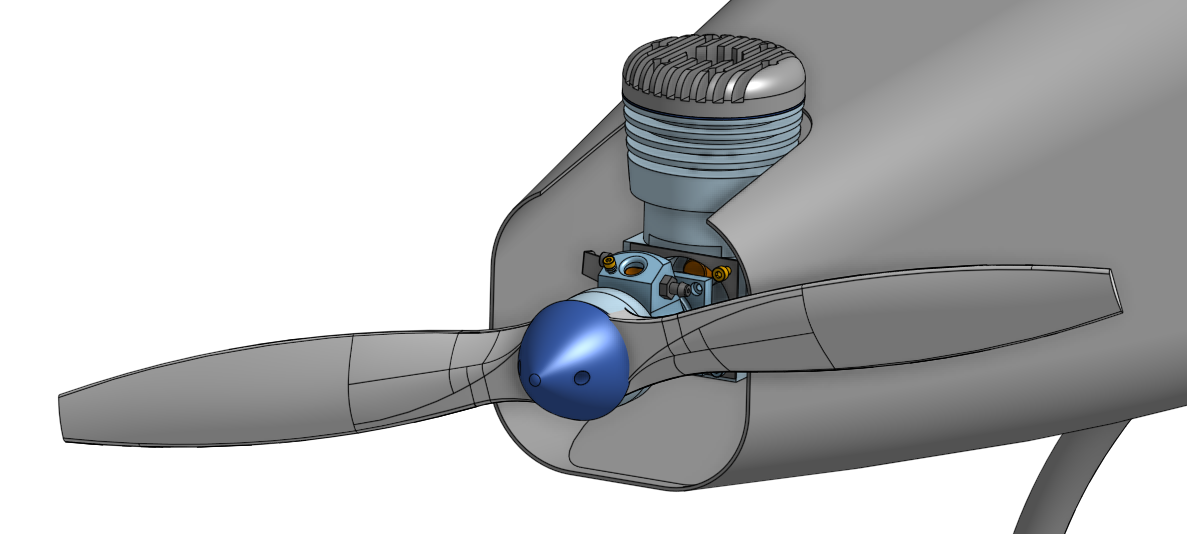
\includegraphics[width = 1\linewidth]{graphics/cad/engineCruiseCut.png}
	\caption{Cut around the cruise engine for the cooler.}
	\label{fig:engineCruiseCut}
\end{figure}

Around these components the fuselage has been created. To fix all components to the fuselage a board is built, displayed in figure \ref{fig:fuseInt1}.

\begin{figure}[ht]
	\centering
	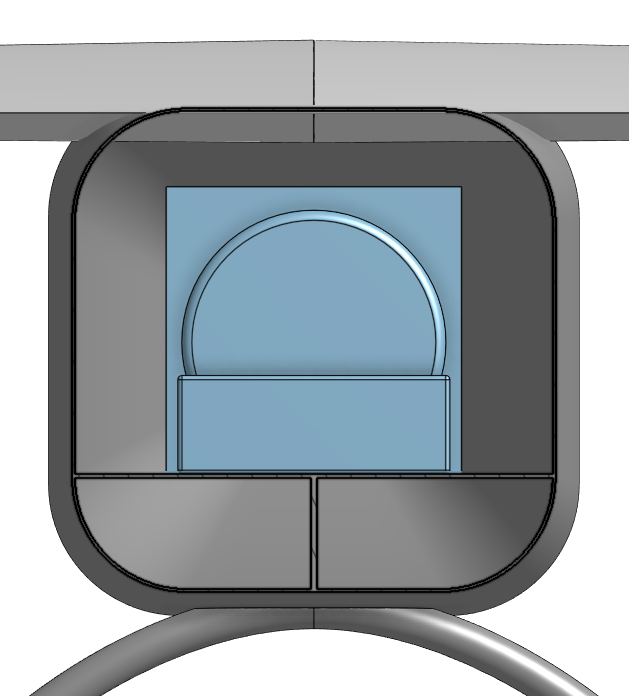
\includegraphics[width = 0.5\linewidth]{fuselageInternal1.png}
	\caption{Board inside the fuselage to accommodate the components.}
	\label{fig:fuseInt1}
\end{figure}

\section{External layout}

The external layout of the fuselage is very important because it is responsible for the main blockage in the air flow around the aircraft. This means it has to obtain a comparatively slender design in addition to a reasonable aerodynamic shape. The result of these considerations is displayed in figure \ref{fig:fuseExt1}.

\begin{figure}[ht]
	\centering
	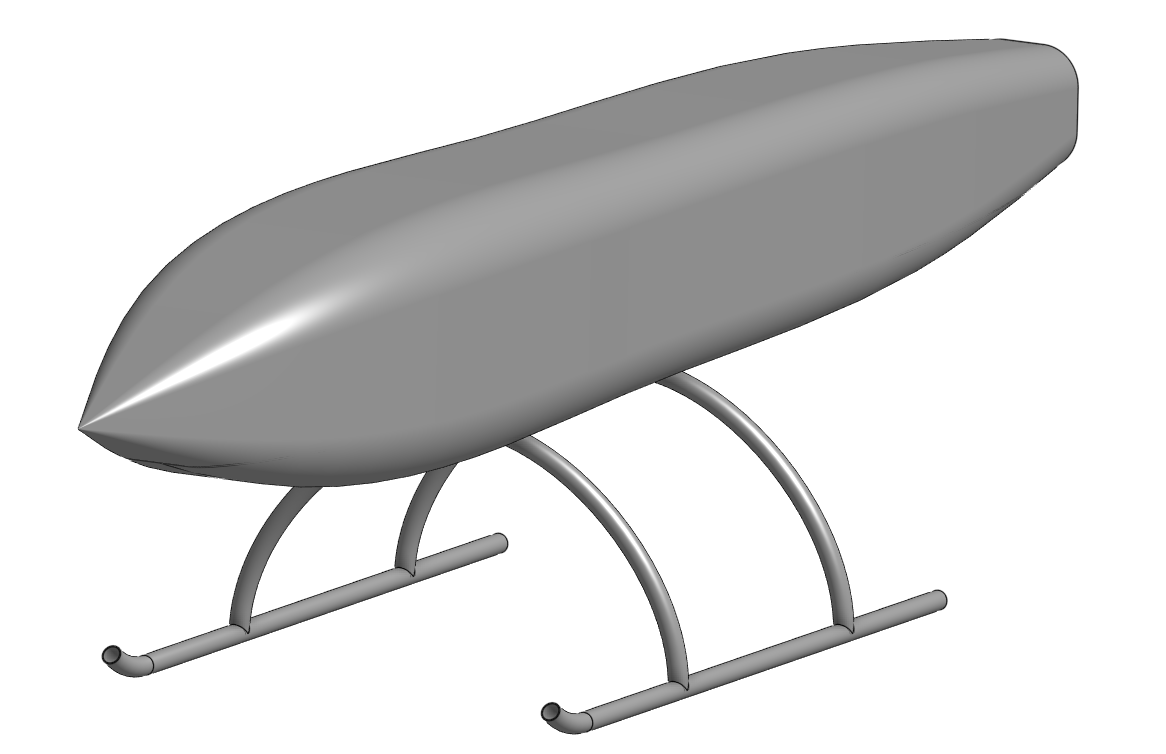
\includegraphics[width = 0.95\linewidth]{graphics/fuselageExternal1.png}
	\caption{Side view on the fuselage.}
	\label{fig:fuseExt1}
\end{figure}

The landing gear of the aircraft is fixed to the fuselage and can not be moved into the fuselage during cruise. The shape of the landing gear is based on landing gears of helicopters. The advantages of this shape are that it provides a stable base when the aircraft is set down on the ground and it is also light and produces a small drag during cruise. The advantage of the tube structure is that it is easily produced and fixed to the fuselage. The circular shape of the connection between the bottom tubes and the fuselage provides similar properties as a spring-damper combination.

The position of the landing gear is close to the centre of gravity, which provides a stable footing for the aircraft when landed. The ground clearance of approximately $240\ \mathrm{mm}$ ensures a safe landing on uneven grounds, see figure \ref{fig:fuseExt2}.

\begin{figure}[ht]
	\centering
	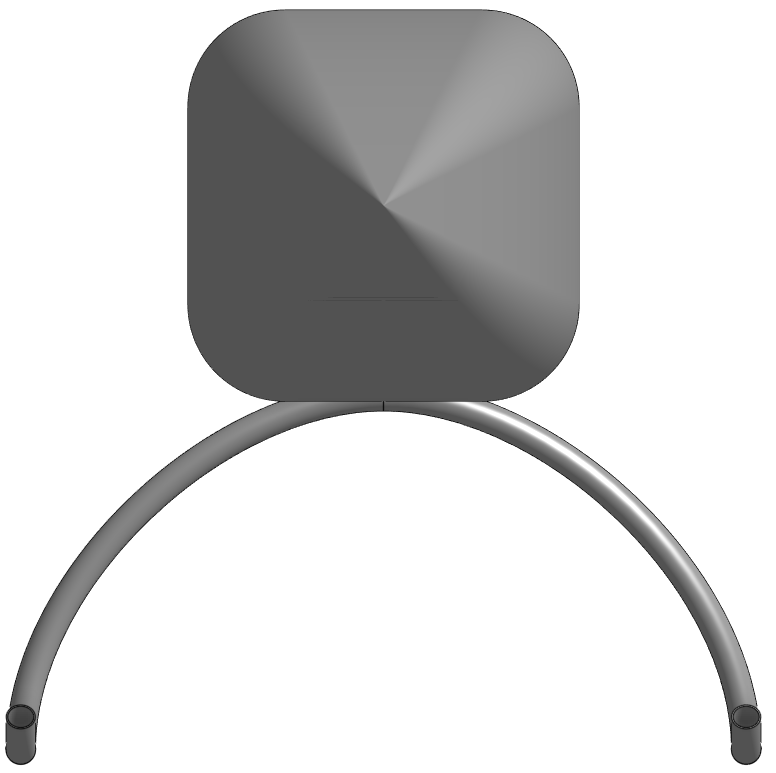
\includegraphics[width = 0.5\linewidth]{graphics/fuselageExternal2.png}
	\caption{Front view on the fuselage.}
	\label{fig:fuseExt2}
\end{figure}

\chapter{Tail Design}

Historically, the tail part of an aircraft has seen a fair amount of variety when it comes to layout, design and positioning within the context of the whole aircraft, whether as a consequence of experimentation or change of the needs of a certain aircraft at the moment of its tail design. The design of the tail can have an important role in the final settings for weight, stability, control and other factors, and all the different designs used historically have a different impact on all of them.

\section{Tail Choice}\label{sec:tailchoice}

Considering the market research done previously and the reference models used, the choice for a tail design was settled on an inverted V-tail configuration, which consists of two separate booms running in parallel to each other. At the end, both ends are connected by the tail wing, a rectangular wing of fixed area in an inverted V setting, which means it is raised at the centre above the vertical position of both root chords. Since the wing is rectangular and has no tip, the chord is constant throughout and is equal to the mean chord $\bar{c}$. This choice was also based on minimising the interference between the rear cruise engine propeller wake and the tail itself.

An example of an inverted V-tail UAV is included in figure \ref{fig:rq7}.
\begin{figure}[ht]
	\centering
	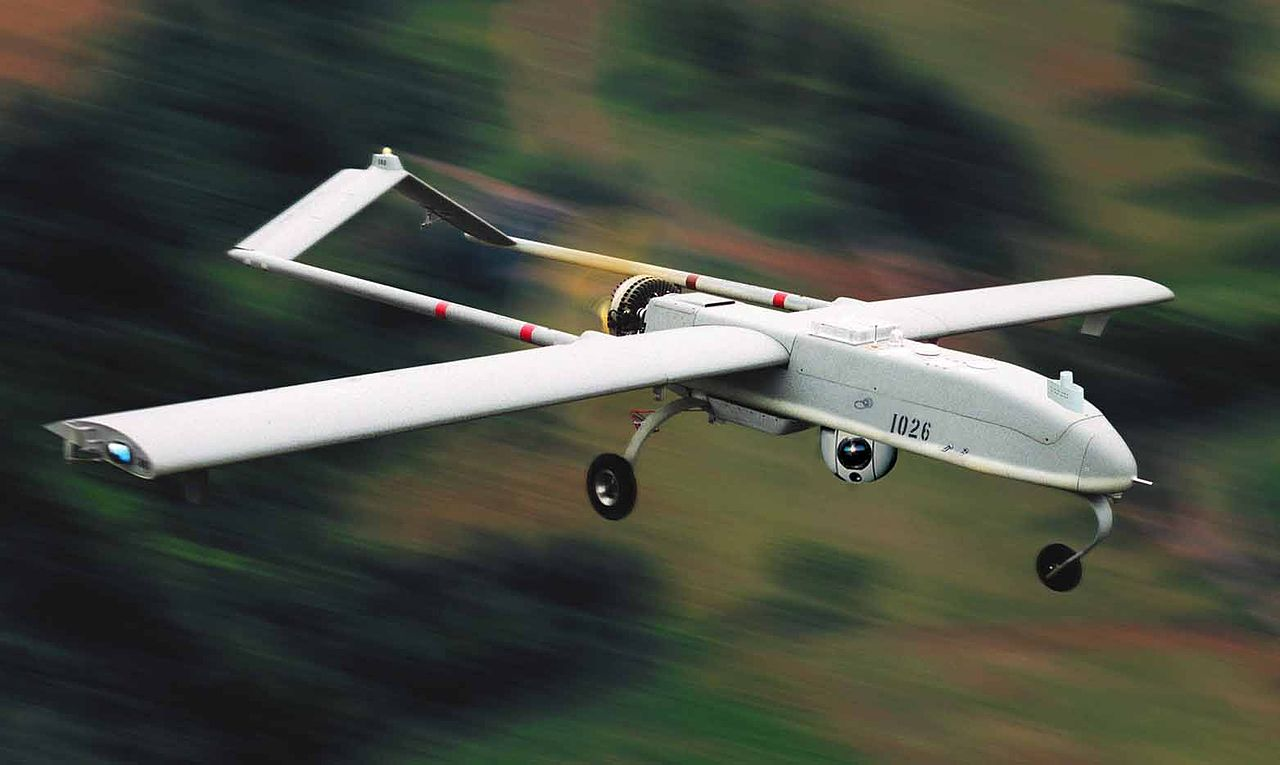
\includegraphics[width = 0.5\linewidth]{USMC-01522.jpg}
	\caption[The \textit{AII RQ-7 Shadow} UAV.]{The \textit{AII RQ-7 Shadow} UAV, an example of military application of an inverted V-tail \cite{olivedrab-rq7}.}
	\label{fig:rq7}
\end{figure}

\section{Tail Sizing}

With the tail configuration set to inverted V-tail, the tail now has to be sized according to the size and current design objectives of the aircraft. The sizing done in the following paragraphs was done using the relations provided in \citetitle{corke} \cite{corke}.

The first variable to be sized was the vertical tail. Using the relation with the wing geometry from the aforementioned reference, which we present in equation \ref{eq:S_VT}, we can determine the vertical tail area.
\begin{gather}\label{eq:S_VT}
	S_{VT} = C_{VT}\frac{b_WS_W}{l_{VT}}
\end{gather}
Also fairly straightforward is the determination of the horizontal tail area, which presents a similar relation.
\begin{gather}\label{eq:S_HT}
	S_{HT} = C_{HT}\frac{\bar{c}_WS_W}{l_{HT}}
\end{gather}
The variables $l$ represent the distance between quarter-chord locations of the mean aerodynamic chord of the main wing and the corresponding stabilizer and $b_W$ and $S_W$ represent the main wing span and area respectively. The value of $C_{VT}$ and $C_{HT}$ varies according to the mission requirements, and can be determined according to aircraft with similar mission requirements. In this case, the values were obtained from table 6.1 from page 123 from \citetitle{corke} \cite{corke}. Assuming the mission requirements to be similar to that of a homebuilt aircraft, the values for the coefficients were $0.04$ for $C_{VT}$ and $0.50$ for $C_{HT}$.

Important to note from the previous equations, all the calculations are being done for the situation of a standard tail. For the situation chosen, an inverted V-tail with a side-by-side H-tail-like configuration, we do not use horizontal and vertical stabilizers, instead relying on two diagonal stabilizers to perform the tasks intended for the original tail configuration.

So what does this entail for the surface area and stabilizer shape calculations? Effectively, the surface area calculations are done in much the same way as done previously in equations \ref{eq:S_VT} and \ref{eq:S_HT}, but since we are working with a single set of symmetrical airfoils instead of horizontal and vertical stabilizers, we can add the area calculated for both and use that as a reference for the total area of the diagonal stabilizers.
\begin{gather}
	S_T = S_{VT} + S_{HT}
\end{gather}

Another important factor to determine is the angle between these two diagonal stabilisers. We are going to place these stabilisers symmetrically, which means the angle between the stabiliser and the aircraft's vertical axis will be the same for both. To define the angle $\nu$, the elevation of each diagonal stabiliser relative to the horizontal plane, we will use an equation from the \citetitle{vleitwerke} \cite{vleitwerke} article.
\begin{gather}
	\nu = \arctan\left(\sqrt{\frac{S_{VT}}{S_{HT}}}\right)
\end{gather}

Using the details we established in section \ref{sec:tailchoice} along with other values we can set the values for the remaining variables.
\begin{figure}[ht]
    \centering
    \begin{tikzpicture}
        \node (boom1) at (0,0) [circle,draw,thick,pattern = crosshatch dots, pattern color = white!60!black, inner sep = 8pt] {};
        \node (boom2) at (6.88,0) [circle,draw,thick,pattern = crosshatch dots, pattern color = white!60!black, inner sep = 8pt] {};
        \coordinate (top) at (6.88/2,6.88/2);
        \path [draw,thin,dashed] (top) -- ++(2,0);
        \path [pattern = dots, pattern color = white!80!black, draw = white!10!black,thin] (top) ++(0:0.7) arc [start angle = 0, end angle = -45, radius = 0.7] -- (top);
        \path [draw, dashed,thin] (boom1) -- node [auto] {$d$} (boom2);
        \path [pattern = dots, pattern color = white!80!black, draw = white!10!black,thin] (top) -- ++(-45:0.7) arc[start angle = -45, end angle = -135, radius = 0.7] -- cycle;
        \path (top) ++(-90:1) node {$\gamma_T$};
        \path (top) ++(-22.5:1) node {$\nu$};
        \path [draw, very thick] (boom1) -- node [auto] {$\frac{b_T}{2}$} (top) -- (boom2);
    \end{tikzpicture}
    \caption[Simplified diagram of the tail design viewed from the back.]{Simplified diagram of the tail design viewed from the back. The CAD version of this diagram can be found in figure \ref{fig:wingFront} of page \pageref{fig:wingFront}.}
    \label{fig:tail_backview}
\end{figure}

Using figure \ref{fig:tail_backview} as a reference, we can get a look at the final layout of the tail. The angle $\gamma_T$ was defined as it was more intuitive and easier to work with for design purposes, and can be easily obtained from $\nu$.
\begin{gather}
    \gamma_T = \pi - 2\nu
\end{gather}
Using the pre-set distance $d$ between booms and the angle $\nu$ we can calculate the total tail wing span $b_T$.
\begin{gather}
    \sin\nu = \frac{d}{b_T}\Rightarrow b_T = \frac{d}{\sin\nu}
\end{gather}
As mentioned in section \ref{sec:tailchoice}, we define the wing shape to be rectangular with a fixed area $S_T$. Using this information we can define the taper ratio $\lambda$ to be $1$ and we can obtain the aspect ratio of the tail.
\begin{gather}
    AR_T = \frac{b_T^2}{S_T}
\end{gather}
Also mentioned previously was the fact that since the wing is rectangular, the chord remains constant throughout. \citetitle{corke} \cite{corke} gives us formulas for both tip and root chord of the tail, but with this property, one of these values should suffice for finding out the missing values.
\begin{gather}
    \bar{c} = c_{tip} = c_{root} = \frac{2S_T}{b_T(1 + \lambda)} = \frac{2S_T}{2b_T} = \frac{S_T}{b_T}
\end{gather}

With all these relations established, we can obtain the necessary values to size the tail, starting with the surface areas.
\begin{subequations}
\begin{gather}
    \begin{aligned}
        S_{VT} = C_{VT}\frac{b_WS_W}{l_{VT}} &= \SI{0.0707}{\meter\squared} \\
        S_{HT} = C_{HT}\frac{\bar{c}_wS_W}{l_{HT}} &= \SI{0.0707}{\meter\squared} \\
        S_T = S_{VT} + S_{HT} &= \SI{0.1637}{\meter\squared}
    \end{aligned}
\end{gather}
This means we can get the angles $\nu$ and $\gamma_T$.
\begin{gather}
    \begin{aligned}
        \mu = \arctan\left(\sqrt{\frac{S_{VT}}{S_{HT}}}\right) &= 0.71692\,rad \\
        \gamma_T = \pi - 2\nu &= 1.7077\,rad
    \end{aligned}
\end{gather}
And finally, the specifications for the tail.
\begin{gather}
    \begin{aligned}
        b_T = \frac{d}{\sin\nu} &= \SI{1.8253}{\meter} \\
        AR_T = \frac{b_T^2}{S_T} &= 20.35 \\
        \bar{c} = c_{tip} = c_{root} = \frac{S_T}{b_T} &= \SI{0.0897}{\meter}
    \end{aligned}
\end{gather}
\end{subequations}

The CAD model of the tail can be see in chapter \ref{chap:cad}.

\section{Tail Airfoil Profile}

We settled on a symmetrical profile for our tail airfoil to prevent it from adding any unwanted lift to our aircraft, but to still allow it to manoeuvre and influence the overall stability of the aircraft.

The chosen airfoil profile was the NACA0012 \cite{naca0012}, which can be seen in figure \ref{fig:naca0012_profile}. Further data can be found in figure \ref{fig:naca0012_data} of page \pageref{fig:naca0012_data}.
\begin{figure}[ht]
    \centering
    \begin{tikzpicture}
        \begin{axis}[ymin = -0.15, ymax = 0.15, grid = both, width = \linewidth, height = 5cm]
			\addplot [mark=none,color=red] table [col sep = space, x index = {0}, y index = {1}] {naca0012.dat};
        \end{axis}
    \end{tikzpicture}
    \caption{NACA0012 symmetrical airfoil profile \cite{naca0012}.}
    \label{fig:naca0012_profile}
\end{figure}

The CAD model of the airfoil can be found in figure \ref{fig:tailCut} of page \pageref{fig:tailCut}.

\chapter{Propulsion} \label{chap:prop}


 One of the requirements for this project was to develop a VTOL UAV with hybrid electric propulsion. Hybrid stands for a mixture of two or more things. In the propulsion case, two technologies are joined to form an alternative propulsion system different form the usual fossil fuel only powered propulsive layouts. Two alternative systems were considered. One consisted in using only one main battery as a source of power to feed all the electric motors, \textit{i.e} the source of power to the cruise engine would be the same batteries as the one that deliver energy to the electric motors for vertical take off and landing. That system would be troublesome as there are not a lot of batteries that can deliver range and endurance values as wanted. That kind of system would not be necessarily called hybrid because no other source of power would be use other that electric. Another alternative would be to use a combustion engine as a generator of power to feed a main battery, and like the previous system, this battery would be the source of power to all 5 electric motors. A system like this one would have a diagram like the one found in \ref{fig:alternative_propulsion_system}. 
 
\begin{figure}[!h]
	\centering
	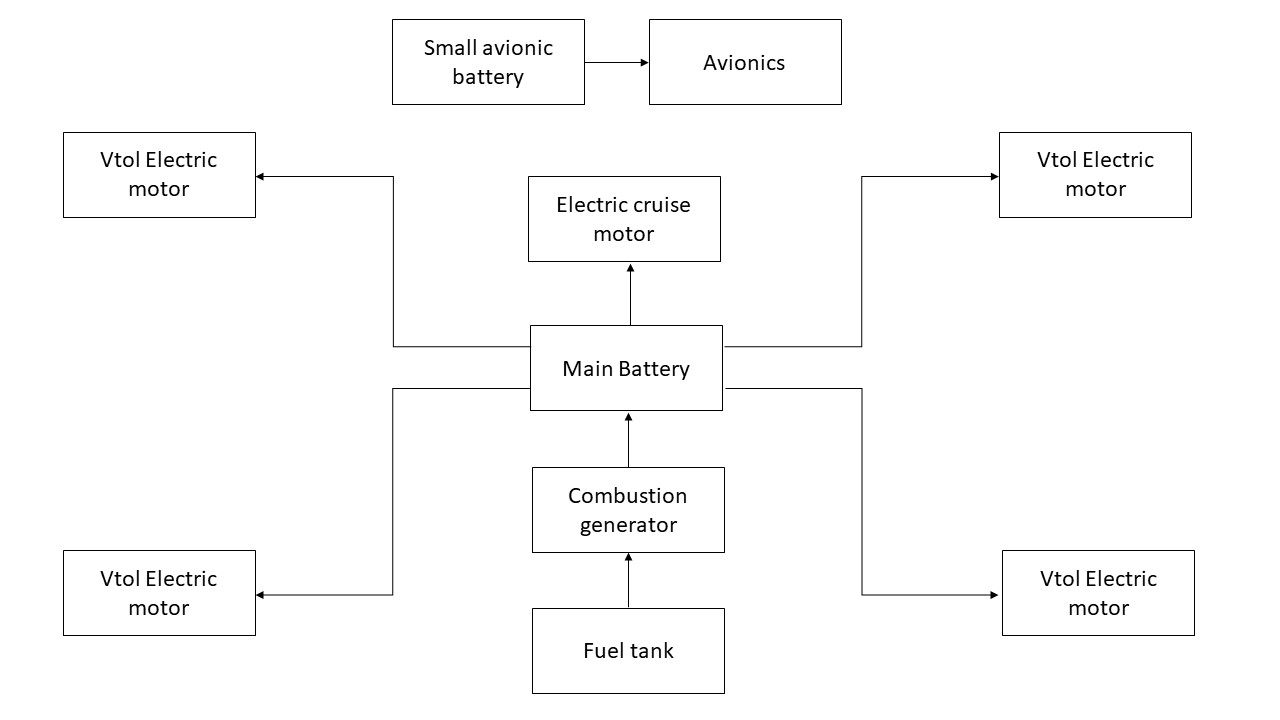
\includegraphics[width = 1\linewidth]{graphics/Alternative_propulsion_system.jpg}
	\caption{Alternative propulsion system}
	\label{fig:alternative_propulsion_system}
\end{figure}

This alternative would, if the right combination of electric motors and generator were chosen, provide the aircraft with the endurance needed, but for the sake of simplicity, and noticing that there are not many generators suitable for aircraft use, a different yet much more simple system layout was selected.  
\begin{figure}[!ht]
    \centering
    \begin{tikzpicture}[node distance = 0.5cm]
        \tikzstyle{component} = [rectangle, draw, align = center, font = \footnotesize, minimum width = 70, minimum height = 30]
        \node at (0,0) (vtolbattery) [component] {VTOL Battery};
        \node (fueltank) [component, above = of vtolbattery] {Fuel tank};
        \node (avionicbattery) [component, below = of vtolbattery] {Small \\ avionic battery};
        \node (combmotor) [component, above = of fueltank] {Combustion \\ motor};
        \node (avionics) [component, below = of avionicbattery] {Avionics};
        \node (motor1) [component, above left = 1.8cm and 3cm of vtolbattery]
        {VTOL \\ electric motor};
        \node (motor2) [component, above right = 1.8cm and 3cm of vtolbattery]
        {VTOL \\ electric motor};
        \node (motor3) [component, below left = 1.8cm and 3cm of vtolbattery]
        {VTOL \\ electric motor};
        \node (motor4) [component, below right = 1.8cm and 3cm of vtolbattery]
        {VTOL \\ electric motor};
        \draw [-{Stealth[]}] (vtolbattery.west) ++(0,0.1) -- ++(-2,0) coordinate (c1) -- (c1|-motor1) -- (motor1);
        \draw [-{Stealth[]}] (vtolbattery.east) ++(0,0.1) -- ++(2,0) coordinate (c2) -- (c2|-motor2) -- (motor2);
        \draw [-{Stealth[]}] (vtolbattery.west) ++(0,-0.1) -- ++(-2,0) coordinate (c3) -- (c3|-motor3) -- (motor3);
        \draw [-{Stealth[]}] (vtolbattery.east) ++(0,-0.1) -- ++(2,0) coordinate (c4) -- (c4|-motor4) -- (motor4);
        \draw [-{Stealth[]}] (fueltank) -- (combmotor);
        \draw [-{Stealth[]}] (avionicbattery) -- (avionics);
    \end{tikzpicture}
    \caption{Propulsion layout.}
    \label{fig:prop_layout}
\end{figure}


As noticeable in figure \ref{fig:prop_layout}, a main battery is used only to feed the VTOL motors, and a usual more conventional gasoline engine is used in the cruise condition. This system allows the complete shut down of the electric system at later flight condition, being more suitable in order to reduce the magnetic interference, studied in a later chapter. 

The next step is to choose the rear cruise engine and respective fuel tank and its propeller, done in section \ref{sec:motorchoice}.

\section{Rear cruise motor choice}\label{sec:motorchoice}

The design point provided us with a needed rear engine power of \SI{2.7723}{\kilo\watt}. A market research was done and the chosen rear engine is the one shown in figure \ref{fig:rcg32cc}. 

\begin{figure}[!ht]
	\centering
	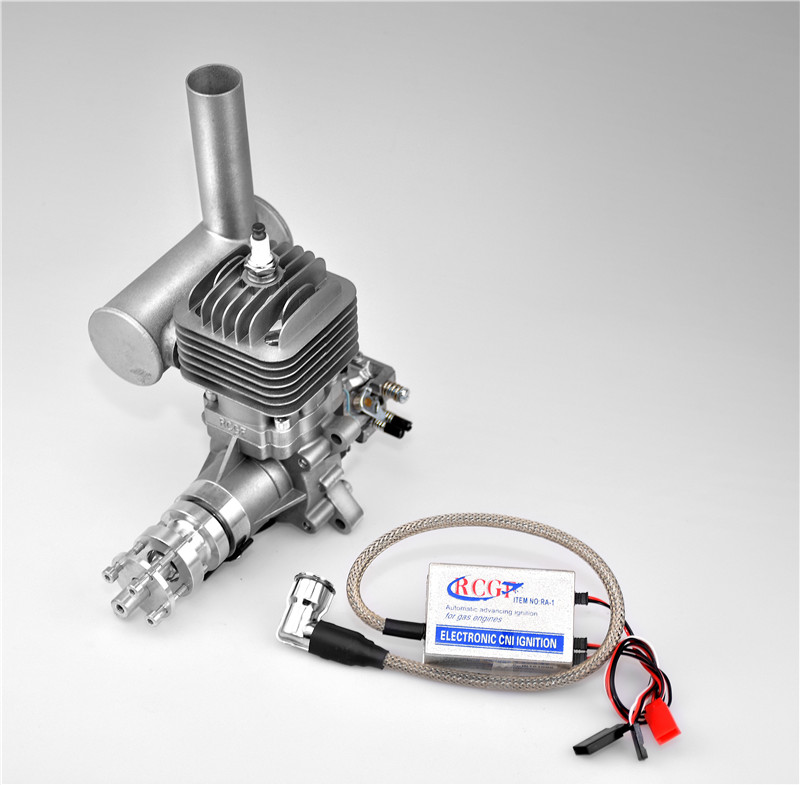
\includegraphics[width = 0.8\linewidth]{graphics/rcg32cc.jpg}
	\caption{RCGF 32cc}
	\label{fig:rcg32cc}
\end{figure}

\begin{figure}[!ht]
	\centering
	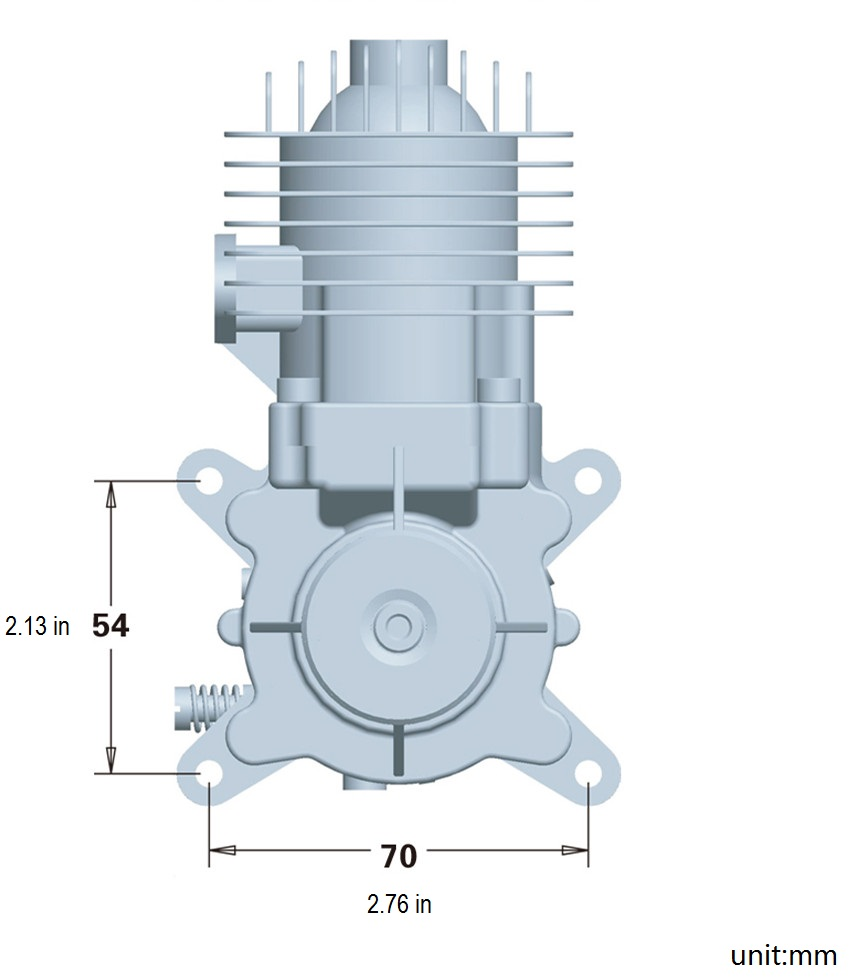
\includegraphics[width = 0.6\linewidth]{graphics/engine_size.jpg}
	\caption{Front view engine dimensions.}
	\label{fig:Front view engine dimensions}
\end{figure}
\begin{figure}[!ht]
	\centering
	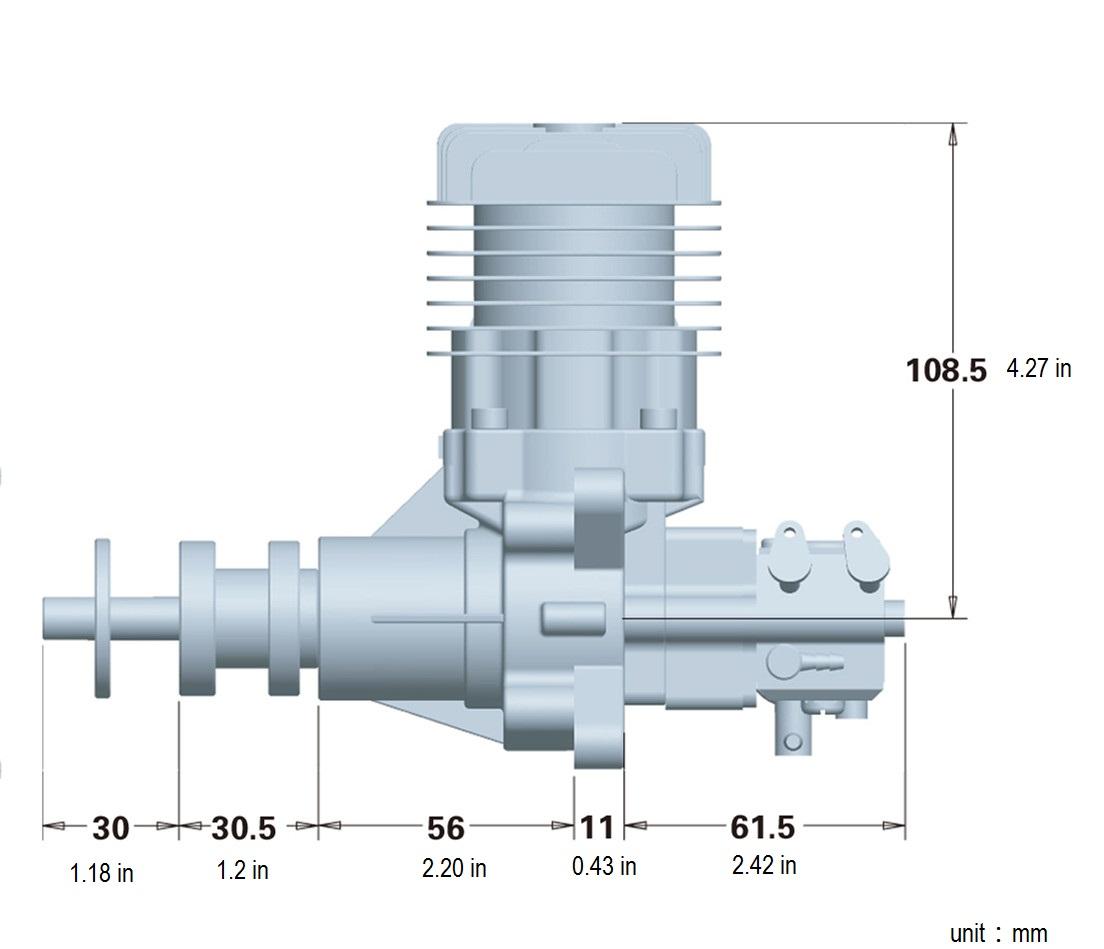
\includegraphics[width = 0.6\linewidth]{graphics/engine_size2.jpg}
	\caption{Lateral dimensions.}
	\label{fig:Lateral dimensions}
\end{figure}
This engine has the following specifications: \cite{rcgf} 
%\begin{itemize}
%    \item Type: 2 cycle piston valve type gasoline engine for airplane
%    \item Piston displacement Cylinder (cc) : 32cc (1.95 cu in)
%    \item Bore x Stroke (mm): 1.5 in(38mm) x 1.2 in (30mm)
%    \item Carburetor : RCGF
%    \item Ignition : DC-CDI (Computer Controlled auto advance, electronic ignition system)
%    \item Power supply: 6-8.4V
%    \item Maximum Output :3.9HP /2.9KW
%    \item Requires: Gasoline, 2-cycle oil, ignition battery and propeller
%    \item speed range : 1500-9000rpm
%    \item Gasoline-Version : Pre-mixed Fuel, 25-40(Gasoline):1 , Recommend:30:1
%    \item Lubrication Oil : 2 cycle engine oil
%    \item Propeller : 19X8 7700rpm (Standard Two leafs prop)
%    \item Suggested Propellers: 18x8, 18x10, 19x8 and 20x8
%    \item Sparking plug: NGK CM6 Type
%    \item Cooling System : Air Cooled
%    \item RCGF engine package Includes: electronic CDI ignition, muffler, spark plug, gaskets, bolts, throttle arm extension \& manual.
%    \item 
%    Weight:
%   \begin{itemize}
%       \item  Engine: 2.05 lb (930 g)
%        \item  Muffler: 3.4 oz (97 g)
%        \item Ignition Module: 4.4 oz (125 g)
%        \item Total: Weight: 2.55 lb (1158 g)
%    \end{itemize}
%    \item Technical Data:
%    \begin{itemize}
%        \item Ignition Battery: 6-8.4 NiCd or NiMH, 6.6V LiFe or 2S LiPo pack
%        \item Gasoline/Oil Mix: 30:1
%        \item  Replacement Spark Plug: NGK CM6 or equivalent
%        \item  Idle Speed: 1800 rpm/min
%        \item Average fuel consumption: 6-7 oz per 15min
%    \end{itemize}
%\end{itemize}

\begin{description}
    \item [Type] 2 cycle piston valve type gasoline engine for airplane;
    \item [Piston displacement Cylinder (cc)] $32cc$ ($1.95\,cu\,in$);
    \item [$\text{Bore}\times\text{Stroke}$ (\si{\milli\meter})] $1.5\,in\,(\SI{38}{\milli\meter})\times1.2\,in\,(\SI{30}{\milli\meter})$;
    \item [Carburator] RCGF;
    \item [Ignition] DC-CDI (Computer Controlled auto advance, electronic ignition system);
    \item [Power supply] \SIrange{6}{8.4}{\volt};
    \item [Maximum Output] $3.9\,HP$/\SI{2.9}{\kilo\watt};
    \item [Requires] Gasoline, 2-cycle oil, ignition battery and propeller;
    \item [Speed range] \numrange{1500}{9000} $rpm$;
    \item [Gasoline-Version] Pre-mixed Fuel, $25$-$40$ (Gasoline):$1$ , Recommend $30$:$1$;
    \item [Lubrication Oil] 2 cycle engine oil;
    \item [Propeller] $19\times8$ \SI{7700}{\rpm} (Standard Two leafs prop);
    \item [Suggested Propellers] $18\times8$, $18\times10$, $19\times8$ and $20\times8$;
    \item [Sparking plug] NGK CM6 Type;
    \item [Cooling System] Air cooled;
    \item [RCGF engine package] Includes: electronic CDI ignition, muffler, spark plug, gaskets, bolts, throttle arm extension \& manual;
    \item [Weight]
    \begin{description}
        \item []
        \item [Engine] \SI{2.05}{\pound} (\SI{930}{\gram});
        \item [Muffler] \SI{3.4}{\ounce} (\SI{97}{\gram});
        \item [Ignition Module] \SI{4.4}{\ounce} (\SI{125}{\gram});
        \item [Total Weight] \SI{2.55}{\pound} (\SI{1158}{\gram});
    \end{description}
    \item [Technical Data]
    \begin{description}
        \item []
        \item [Ignition Battery] \numrange{6}{8.4} NiCd or NiMH, \SI{6.6}{\volt} LiFe or 2S LiPo pack;
        \item [Gasoline/Oil Mix] $30$:$1$;
        \item [Replacement Spark Plug] NGK CM6 or equivalent;
        \item [Idle Speed] \SI{1800}{\rpm}
        \item [Average fuel consumption] \SIrange{6}{7}{\ounce} per \SI{15}{\minute};
    \end{description}
\end{description}

With this level of power, the assign power output of the engine provide the aircraft with a power safety factor of
\begin{gather*}
    \text{Safety factor} = \frac{2.9}{2.7723}-1 \cdot 100 = 4.61 \%
\end{gather*}
Although this seems like a low value, a low value of $\eta_p=0.4$ was assumed already as a safety margin. Further computations will validate this assumption. 
 \newpage 
\section{Rear engine propeller}
Regarding the propeller, the engine specifies some recommended sizes ($18\times8$, $18\times10$, $19\times8$ and $20\times8$). A $20\times8$ propeller was selected.

\begin{figure}[!ht]
	\centering
	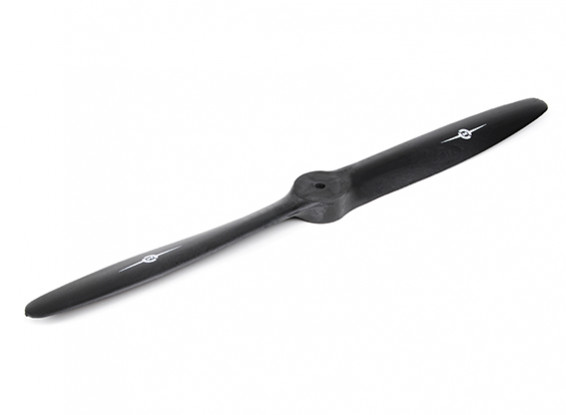
\includegraphics[width = 0.8\linewidth]{graphics/Rear_engine_propeller.jpg}
	\caption{Rear engine propeller by Master airscrew }
	\label{fig:Rear engine propeller}
\end{figure}

It is now relevant to check if such combination of motor and propeller provide the aircraft with reasonable levels of thrust, whenever in static or cruise conditions. For that, formulas from \citetitle{corke} \cite{corke} were used, and the following reasoning was made. 

$\eta_p=0.4$ and $P = \SI{2.9}{\kilo\watt}$, so in order to get the maximum thrust at cruise, the computations will be made assuming a rotational velocity of \SI{9000}{\rpm}, or \SI{150}{\rps}. The rotor radius is $20$ inches, which equals \SI{508}{\milli\meter}. So:
\begin{gather}
    J=\frac{V}{n \cdot D}
\end{gather}
Let $V$ be the cruise speed, \SI{30}{\meter\per\second}, $n$ the rotation velocity in rotations per second, and $D$ the propeller radius. Thus
\begin{gather}
    J=0.3937
\end{gather}
As $C_p$ is calculated with the following equation
\begin{equation}
    C_p=\frac{P}{\rho \cdot n^3 \cdot D^5}
\end{equation}
P being the power and $rho = \SI{1.225}{\kilogram\per\meter\cubed}$ at sea level. Hence,
\begin{gather}
    C_p=0.0207
\end{gather}
Relating $C_p$ and $C_t$ with the following equation:
\begin{equation}
    \eta_p=J \cdot \frac{C_T}{C_P}
\end{equation}
We can get a $\frac{C_T}{C_P}=1.0145$. With this value, the maximum thrust at cruise condition follows from this equation: 
\begin{align}
    \begin{aligned}
	    T&=\frac{P}{n \cdot D} \cdot \frac{C_T}{C_P} \\
	    &= \SI{38.6}{\newton}
	\end{aligned}
\end{align}
For the static conditions, altought the projected aircraft will have no need to take off from the ground with the propulsion of the rear engine, the transition from hovering to cruise will be made with the assistance of the combustion engine and the VTOl electric motors, so it is interesting to know what is the static thrust that this configuration will provide. Thus, using graph 7.6 from \citetitle{corke} \cite{corke} with a $C_P=0.0207$ and making the respective correction for 2 blades using this equation: 
\begin{equation}
	\left(\frac{C_T}{C_P}\right)_{\text{Corrected}}=\left(0.03(NB-3)+1\right) \cdot \frac{C_T}{C_P}
\end{equation}
And using the equation for the thrust used before for the cruise condition, the aircraft is able to produce a thrust of \SI{107.05}{\newton} while stationary with the motor at maximum power.

The rotational speed in maximum power condition is then: 

$$V_{tip}=\sqrt{(pi\cdot n \cdot D)^2 + (Vcr)^2} = 241.262$$m/s
which corresponds, at sea level, to a tip mach of 0.7, lower that the 0.85 restriction due to noise levels. 
\section{Fuel tank}

Finally the last component that needs to be analysed in the combustion part of the propulsive system is the fuel tank. Based on the data provided by the engine manufactured, this engine consumes around \SI{6}{\ounce} if gasoline every 15 minutes of flight. Due to the lack of information regarding this value, the \SI{6}{\ounce} for \SI{15}{\minute} will be used in the fuel tank calculations. 

6oz, in the metric system, are \SI{170}{\milli\gram} of fuel. Thus, per hour, this engine is estimated to burn \SI{680}{\gram} of gasoline. As the aircraft is projected to have a $5$ hour endurance, the fuel needed to accomplish the mission is \SI{3400}{\gram}. The average gasoline density is \SIrange{715}{780}{\kilogram} per cubic meter, so \SI{3400}{\gram} of gasoline result in 
\begin{gather*}
    \text{Fuel} = \frac{1000\cdot 3.4}{780} = 4.35\,\text{liters}
\end{gather*}

As a safety margin, a larger fuel tank was chosen, with a maximum capacity of $4.8$ liters. 
\begin{gather*}
    \text{Safety factor} = \left(\frac{4.8}{4.35}-1\right)\cdot100=10.3\%
\end{gather*}

The fuel tank is the one found in figure \ref{fig:fuel tank}.

\begin{figure}[!ht]
	\centering
	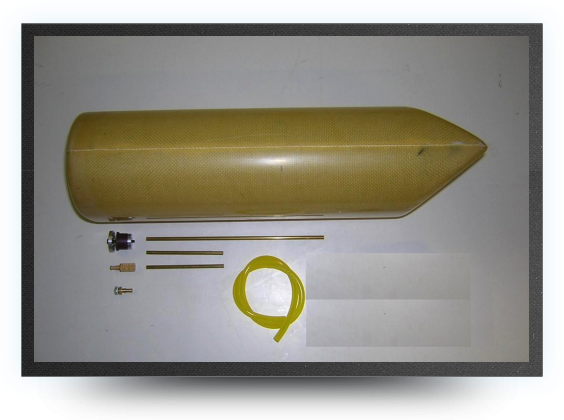
\includegraphics[width = 0.8\linewidth]{graphics/Fue_tank.png}
	\caption{Rear engine kevlar fuel tank - ADR 4.8 \cite{fueltank}.}
	\label{fig:fuel tank}
\end{figure}

 The tank is \SI{360}{\milli\meter} long and has a diameter of \SI{130}{\milli\meter}. with all the included components (tubes, valves), it was assumed that the empty weight is \SI{0.5}{\kilogram} and the full weight is \SI{4}{\kilogram}, for the calculations in the following chapters.



\newpage
\section{Brushless Motors for VTOL}
In chapter \ref{chap:rotordesign} we theoretically calculate the characteristics of the rotors to use in our UAV. In this section we intend to find rotors commercially available that meet these characteristics.  The following conclusions have already been reached:
\begin{itemize}
    \item Number of Rotors = 4
    \item Combined Thrust to Hover = \SI{404.7}{\newton}
    \item Rotor Radius = \SI{0.3092}{\meter} = \SI{30.92}{\centi\meter}
    \item Rotor Diameter = $30.92\times 2$ = \SI{61.84}{\centi\meter}
    \item Number of Blades = 2
\end{itemize}

This means that we will have to look at market for rotors with the following properties:

\begin{gather}
    \text{Thrust (for 2 Blades)}=\frac{\text{Combined Thrust to Hover}}{\text{Number of Rotors}}=\frac{404,7}{4}=\SI{101.2}{\newton} \\
    \text{Rotor Diameter} = \SI{61.84}{\centi\meter} \approx \SI{24.35}{\inch}
\end{gather}
 
During the market research we quickly concluded that the best solution would be a brushless motor. Brushless Electric Motors are synchronous motors powered by DC electricity via an inverter or switching power supply which produces an AC electric current to drive each phase of the motor via a closed loop controller. The controller provides pulses of current to the motor windings that control the speed and torque of the motor.\par
From the various options available in the market we selected the brushless motor $KDE7215XF-135$ (Figure \ref{fig:motorkde}) of the brand KDE Direct that is recognized by its high-quality and engineered motors, specific for multi-rotor and UAS applications and designed to provide high performance and zero-vibration operations.


\begin{figure}[ht]
    \centering
    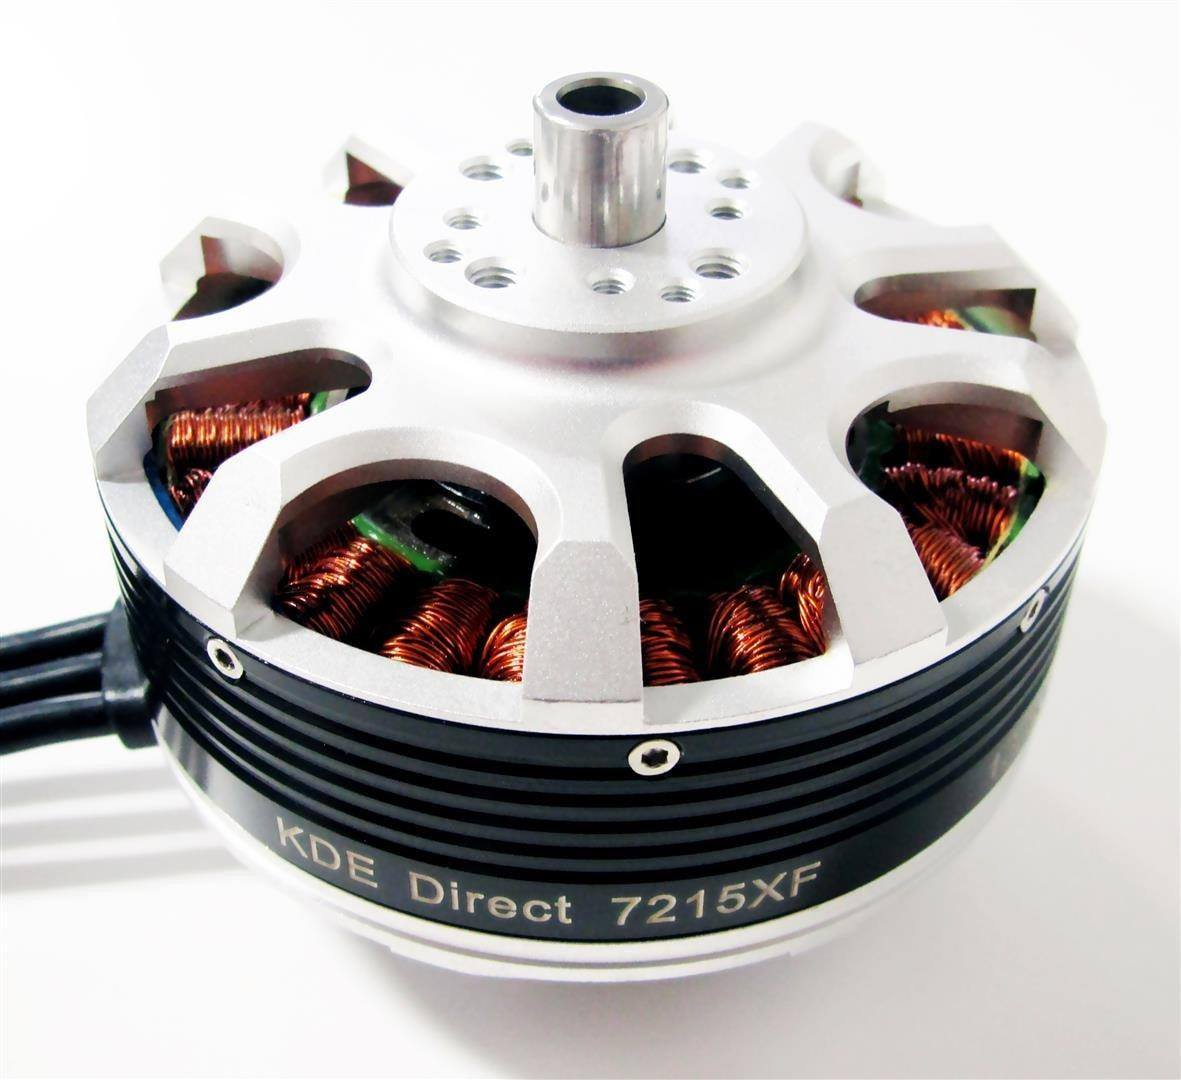
\includegraphics[width=0.5\textwidth]{graphics/BrushlessMotorsforVtol/x.jpg}
    \caption{$KDE7215XF-135$ Brushless Motor}
    \label{fig:motorkde}
\end{figure}
\newpage 
Performance parameters of this brushless electric motors:
\begin{itemize}
    \item $Kv$ (Motor Velocity Constant): $135 RPM/V$
    \item $Kt$ (Motor Torque Constant): $0.0707\,Nm/A$
    \item $Km$ (Motor Constant): $0.2774\,Nm/\sqrt{W}$
\end{itemize}

\begin{figure}[ht]
    \centering
    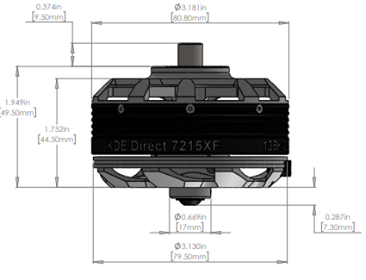
\includegraphics[width=0.5\textwidth]{graphics/BrushlessMotorsforVtol/y.png}
    \caption{Dimensions of the $KDE7215XF-135$ Brushless Motor}
    \label{fig:kdedimensions}
\end{figure}

When fed by batteries of type $12S$ and when equipped with 2 propeller blades with the diameter $24.5$ inches (which is almost exactly the theoretical value calculated) each of these rotors can generate a thrust of \SI{126.02}{\newton}, according to figure \ref{fig:performancekde}, that is greater than the required \SI{101.2}{\newton} and which validates our choice.

\begin{figure}[ht]
    \centering
    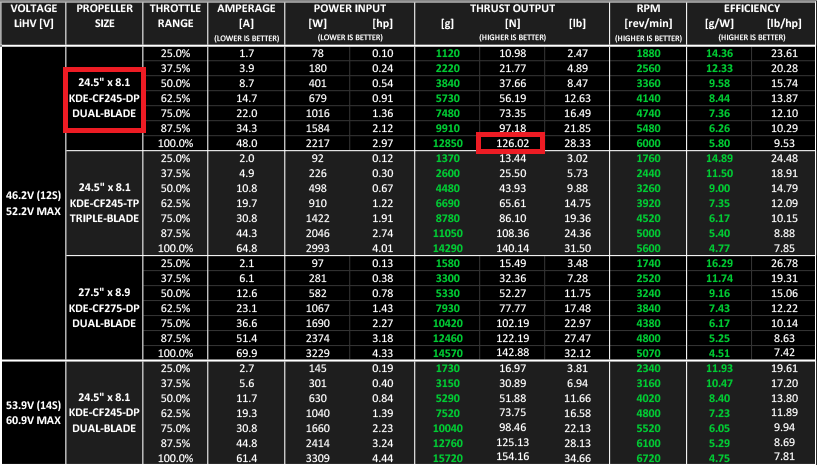
\includegraphics[width=\textwidth]{graphics/BrushlessMotorsforVtol/z.png}
    \caption{Performance Data of the KDE7215XF-135 Brushless Motor}
    \label{fig:performancekde}
\end{figure}
\newpage 
\section{Propeller Blades for the Brushless Motors}
Since we have chosen to use brushless motors due to the numerous advantages they present and that we have already mentioned in the previous section, we need to choose propeller blades suitable to produce the desired Thrust. In chapter \ref{chap:rotordesign} we determined that the theoretical radius of the rotors should be \SI{30.92}{\centi\meter} which corresponds to a diameter of \SI{61.84}{\centi\meter} that is approximately $24.35$ inches. \par
As we saw in the table shown in figure \ref{fig:performancekde}, the brushless motor chosen supports propeller blades with $24.5$ inches, which is almost exactly the theoretical value calculated for the diameter of the rotors. Therefore, we can use the $KDE$-$CF245$-$DP$ propeller blades that together with the motor form a rotor with \SI{31.115}{\centi\meter} of radius (which is very close to the theoretically value calculated) and which generate a thrust of \SI{126.02}{\newton}, greater than the \SI{101.2}{\newton} required. 

It is also assumed that these rotors are able to feather with the airflow when they are not is use, to reduce their drag in cruise conditions. 

\begin{figure}[ht]
    \centering
    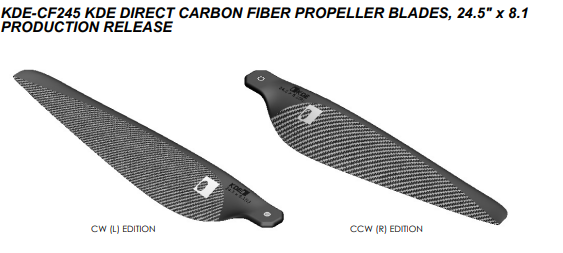
\includegraphics[width=0.8\textwidth]{graphics/BrushlessMotorsforVtol/propellerblades.png}
    \caption{$KDE$-$CF245$-$DP$ propeller blades.}
    \label{fig:propblades}
\end{figure}

\begin{itemize}
    \item Material: Carbon-Fiber
    \item Weight: $34.9\,g$/blade (design is FEA optimized for maximum strength and minimum weight).

\end{itemize}

\begin{figure}[ht]
    \centering
    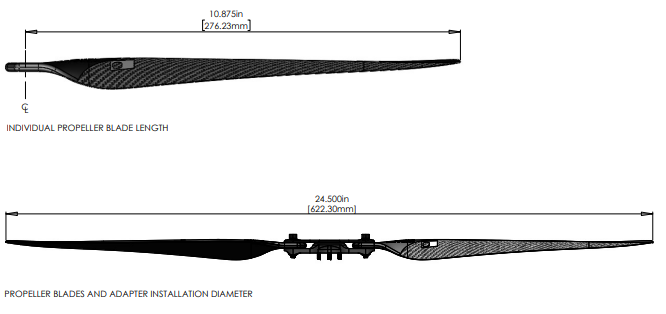
\includegraphics[width=\textwidth]{graphics/BrushlessMotorsforVtol/propblades2.png}
    \caption{Dimensions of the $KDE$-$CF245$-$DP$ propeller blades.}
    \label{fig:propblades2}
\end{figure}


\chapter{Power Storage}\label{chap:power}
In order to store the required power for the Vertical Take-Off and Landing steps and to feed the avionics systems it’s necessary to have batteries. The batteries store the energy for the hover stages and for the operation of the electronic components and give them proper voltages and currents. In this section we will present the commercially available batteries chosen to incorporate into our UAV. 
\section{Battery for Hover}
In chapter \ref{chap:bathover} we had already determined the main properties of this battery:

\begin{itemize}
    \item $W_{\text{battery}} = \SI{2.2447}{\kilogram}$;
    \item $E_{\text{bat}}=\SI{165}{\watt\hour\per\kilogram}$, i.e.\@ Energy specific density for the batteries of \SI{165}{\watt\hour\per\kilogram};
    \item Battery Storage Capacity = $165\times2.2447=\SI{403.755}{\watt\hour} = \SI{403.755}{\volt\ampere\hour}$.
\end{itemize}
	
When we chose the brushless motors and their propeller blades, we concluded that we needed a $12S$ type battery, that is, a battery capable of delivering a $44.4V$ output voltage.
	
\begin{itemize}
    \item Battery Type: $12S$
    \item Battery Output Voltage: $44.4V$
\end{itemize}


Once the battery voltage is known, it is possible to convert the storage capacity from VAh to mAh, which is the unit used commercially. Through equation \ref{eq:batstorcapacity2} we determine that the battery must have at least $9094$ mAh.


\begin{equation} \label{eq:batstorcapacity2}
    \text{Battery Storage Capacity }[mAh]=403.775\ [VAh]\ 44.4\ [V]\times 1000=9094 mAh 
\end{equation}


Considering all the requirements listed above, we select the MaxAmps LiPo $10900$, $12S$, $44.4v$ Battery Pack.

\begin{figure}[ht]
    \centering
    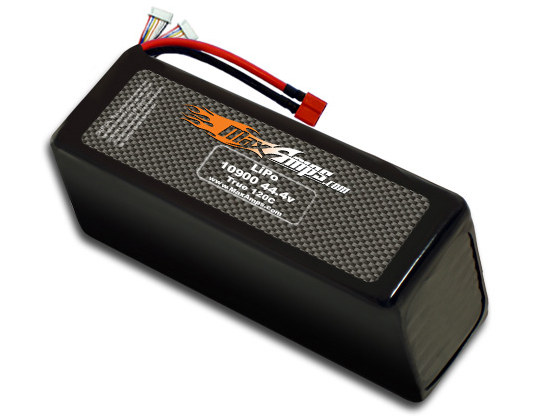
\includegraphics[width=0.49\textwidth]{graphics/BrushlessMotorsforVtol/powerstorage.png}
    \caption{MaxAmps LiPo 10900, 12S, 44.4v Battery Pack}
    \label{fig:powerstorage}
\end{figure}
\newpage
This Battery Pack has the following technical features:
\begin{itemize}
    \item $10.900\,mAh$ capacity
    \item Type: $12S$
    \item Output Voltage of $44.4$ volts
    \item True $120C$ rating
    \item $100\%$ waterproof
    \item Dimensions: $137mm \times 45mm \times 209mm$
    \item Weight: $2727g$
\end{itemize}

\section{Small Battery for servos and avionics:}
Since we also need avionics and servo actuators in our UAV, we chose another small battery, with a lower output voltage and a lower capacity, to feed these electronic components.\par

\begin{figure}[ht]
    \centering
    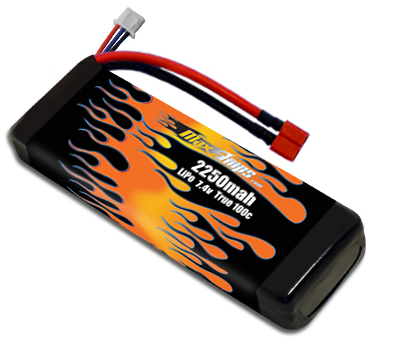
\includegraphics[width=0.49\textwidth]{graphics/AVIONICS/bat2.png}
    \caption{MaxAmps LiPo 2250, 2S, 7.4v Battery Pack}
    \label{fig:bat2}
\end{figure}
\newpage
This Battery Pack has the following technical features:
\begin{itemize}
    \item 2250mah capacity
    \item Type: 2S 
    \item Output Voltage: 7.4 volts
    \item True 100C rating
    \item 100\% waterproof
    \item Dimensions: 100mm \times 35mm \times 16mm
    \item Weight: 121g
\end{itemize}

\chapter{Aerodynamic simulations}\label{chap:Aerodynamic simulations}

\begin{figure}[!ht]
	\centering
	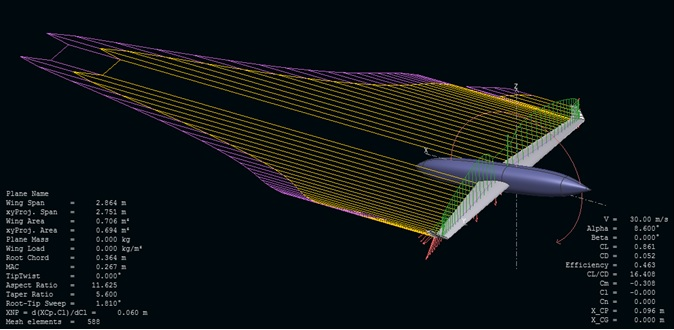
\includegraphics[width = 0.8\linewidth]{graphics/Aero_simulation_flight_cruise.png}
	\caption{Aerodynamic simulation in cruise flight}
	\label{fig:Aero_simulation_flight_cruise}
\end{figure}

Estimation of the total weight of the aircraft at the beginning of the cruise and determination of the $C_l$ :

\begin{equation}
    W_{max} = 34 \cdot 9.81 = 333.54 N
\end{equation}

\begin{equation}
    L = \frac{1}{2} C_{L} {V_{cr}}^2 S_{w}\ \rho_{sea}\Longrightarrow C_{l}\approx0.857
\end{equation}

Estimation of the angle of attack required to obtain the necessary $C_L$:
\begin{equation}
    \alpha = 8.6 \degree \rightarrow \begin{cases} C_{l} = 0.861 \\ C_{d} = 0.052 \end{cases}
\end{equation}

In cruising flight, the thrust should equal the drag and the thrust required must be lower than the combustion engine can provide:
\begin{equation}
    T = D = \frac{1}{2} C_{D} {V_{cr}}^2 S_{w}\ \rho_{sea} = 20.24 N 
\end{equation}

\begin{equation}
    T_{available} = \frac{\eta P}{V_{cr}} = 38.6N
\end{equation}

Using the $XFLR5$\textregistered{}  program, the angle of attack was estimated in the initial phase of the cruise. Having obtained the value of $8.60\degree$. It was also estimated drag in this flight situation in which the value of $20.24\,N$ lower than the $38.6\,N$ capable of being generated was obtained. However, it should be noted that this simulation only took place considering the main wing and the fuselage due to program limitations. So the total drag of the configuration should be around $30\,N$ (which represents $77.72 \%$ of the thrust available to be made by the engine) This value comes from an over estimation of 5N due to the tail drag and another 5N from the VTOL components and boom structure. This shows an over sizing, as an engine with less power could have been used, in order to obtain a lower consumption and consequently lower weight of the configuration. However, due to the fact that it was limited to the existing solutions in the market, the engine shown in the propulsion chapter was chosen, because it respects the required requirements.

\section{Drag tail estimation}

The drag estimation due to the tail wing installation on the aircraft was estimated using the XFLR5 program. Because of some limitation of the program, the estimated drag corresponds to the induced drag in the case of the main wing + wing tail in non-viscous fluid. Since the tail wing is a fuselage body, the main drag component generated will be the induced component.

\begin{figure}[!ht]
	\centering
	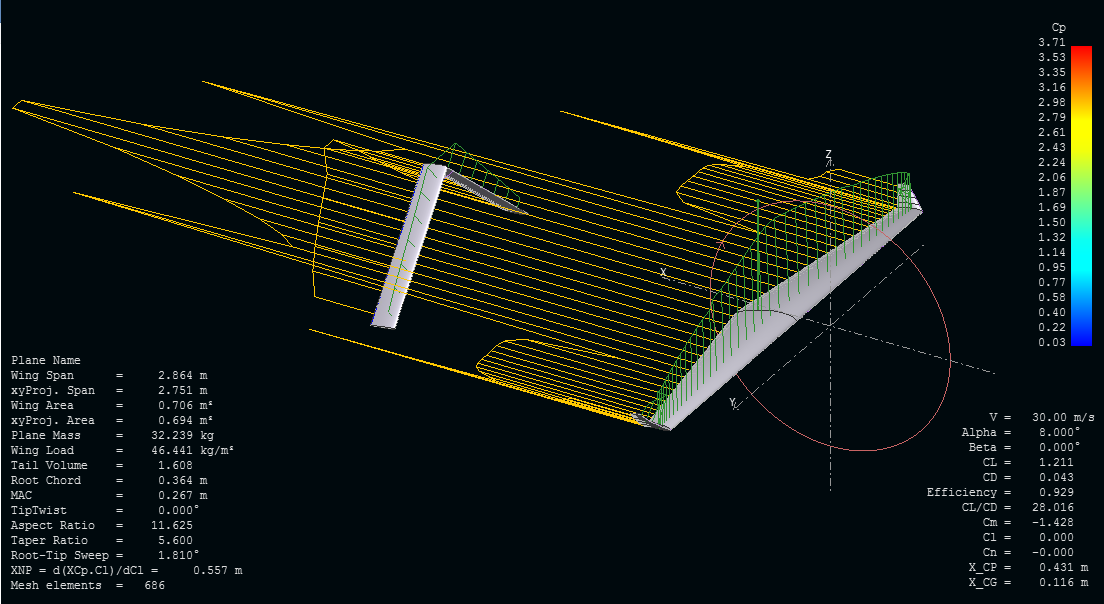
\includegraphics[width = 0.8\linewidth]{graphics/aero_simulation_drag_w+wingtail.png}
	\caption{Induced drag (Case main wing and tail wing)}
	\label{fig:drag_w_wtail}
\end{figure}

\begin{figure}[!ht]
	\centering
	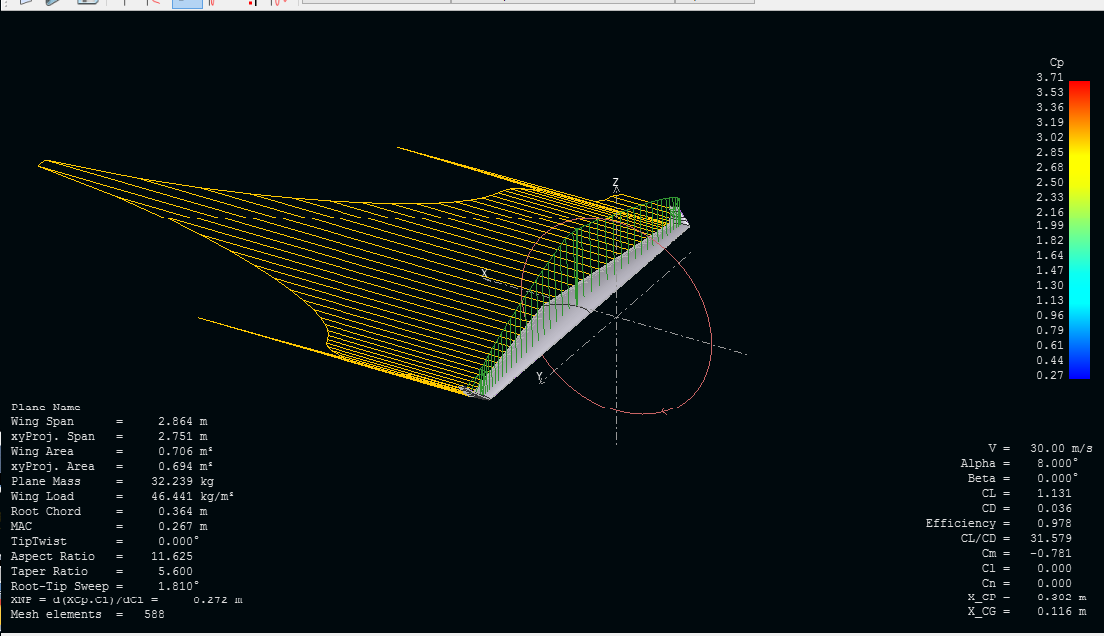
\includegraphics[width = 0.8\linewidth]{graphics/aero_simulation_drag_wing.png}
	\caption{Induced drag (Case main wing)}
	\label{fig:drag_wing}
\end{figure}

It can be observed in \ref{fig:drag_w_wtail} and \ref{fig:drag_wing} that the induced drag (case main wing + tail wing) has a value of 0.43, which shows an increase around $20$ and $25$ percent compared with (case only main wing) that has the value of 0.36 for the drag induced. These results were used to help in the estimation of total drag.

\section{Comparison of wing chosen with elliptical wing}

The distribution of circulation along the span, for a given lift, which produces a minimum induced resistance, defined by expression \ref{eq. induced drag} is an elliptic distribution.

\begin{equation}
    C_{Di} = \frac{C_{L}^2}{\pi e AR}
    \label{eq. induced drag}
\end{equation}

However elliptical wings, which are capable of generating this support distribution, have two drawbacks:

\begin{itemize}
	\item One is the fact that wings of this type are more difficult to construct and therefore are more expensive.
	\item The other reason has to do with safety and control of the flight, with all the profiles working at the same angle, when the alpha is increased too much, the stall occurs along the entire wing simultaneously.
\end{itemize}

For these reasons a trapezoidal wing was chosen as an alternative since it is easier to construct and has a lift distribution that approaches the elliptic distribution. 

In addition, a solution chosen to minimize induced drag was to install winglets, because allow to reduce air flow at the marginal edge due to the pressure gradient. On the other hand, the winglets act as lift components, which improve the efficiency of the wing.Since the wing becomes behaving like a wing with greater wingspan. This allows to reduce bending moments in the recess due to having a shorter wing.

\begin{figure}[!ht]
	\centering
	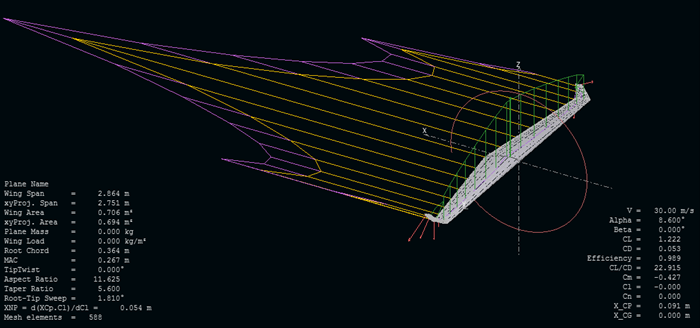
\includegraphics[width = 0.65\linewidth]{graphics/Aero_simulation_wing_chosen.png}
	\caption{Aerodynamic simulation of chosen wing}
	\label{fig:simulation_chosen_wing}
\end{figure}

\begin{figure}[!ht]
	\centering
	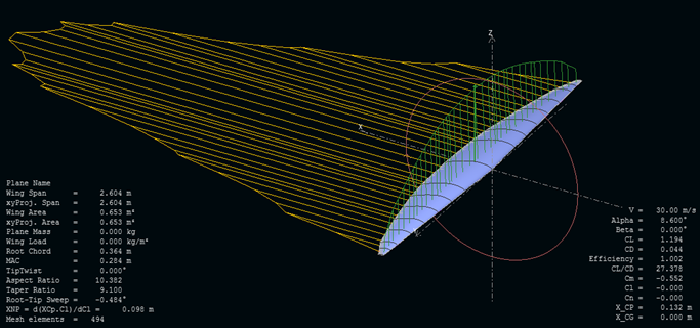
\includegraphics[width = 0.65\linewidth]{graphics/Aero_simulation_wing_elliptic.png}
	\caption{Aerodynamic simulation of elliptic wing}
	\label{fig:simulation_elliptic_wing}
\end{figure}

\begin{figure}[!ht]
    \centering
    	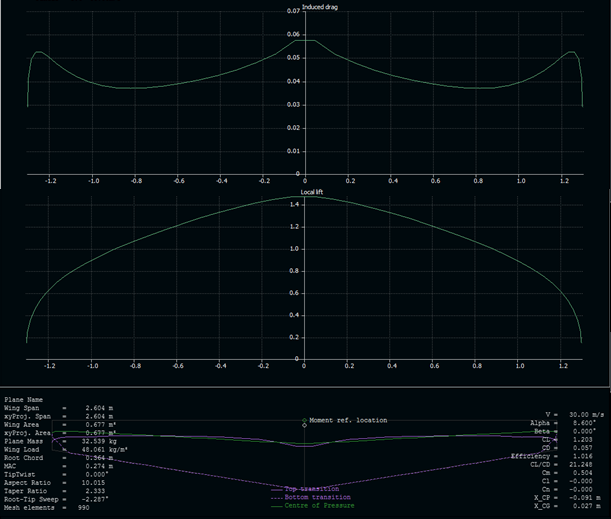
\includegraphics[width = 0.55\linewidth]{graphics/aero_simulation_withoutwinglets(induced).png}
    \caption{Lift distribution and induced drag along the wing (chosen wing without winglets)}
    \label{fig:simulation_withoutwinglets_induced}
\end{figure}
\begin{figure}[!ht]
    \centering
    	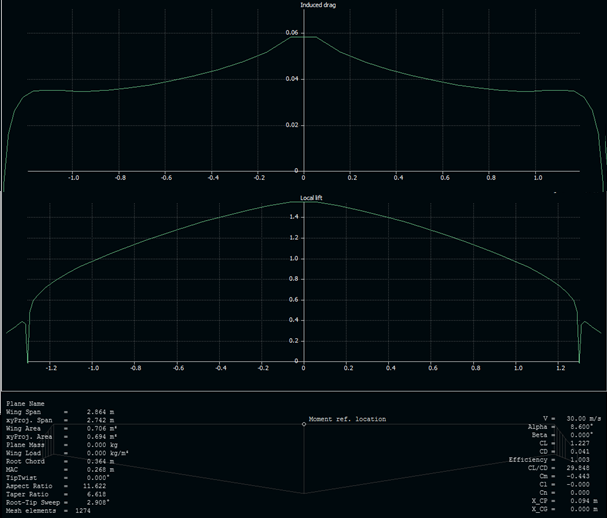
\includegraphics[width = 0.55\linewidth]{graphics/aero_simulation_chosen(induced).png}
    \caption{Lift distribution and induced drag along the wing (chosen wing)}
    \label{fig:simulation_chosen_wing_induced}
\end{figure}

\begin{figure}[!ht]
    \centering
    	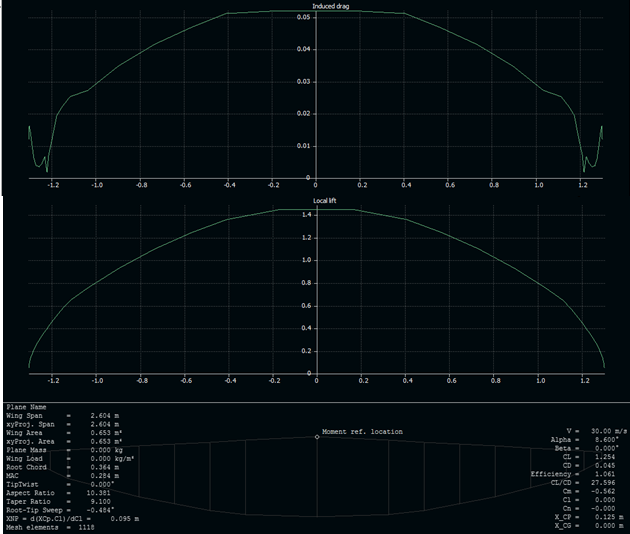
\includegraphics[width = 0.55\linewidth]{graphics/aero_simulation_elliptic(induced).png}
    \caption{Lift distribution and induced drag along the wing (elliptic wing)}
    \label{fig:simulation_elliptic_wing_induced}
\end{figure}

Comparing the presented in the previous figures (\ref{fig:simulation_withoutwinglets_induced}, \ref{fig:simulation_chosen_wing_induced} and \ref{fig:simulation_elliptic_wing_induced}), it can be concluded that the lift distribution along the selected wing approaches the ideal distribution generated by the elliptical wing. It should be noted that in the case of the wing with winglets, this has an increase of lift in wing tips. 

On the other hand, comparing the figures for their induced drag distributions. It can be observed that the wing with winglets has an induced drag distribution that approaches more of the elliptical distribution than the case without the winglets. However, the differences between induced drag distributions are still visible.

%\begin{figure}[!ht]
   % \centering
    %	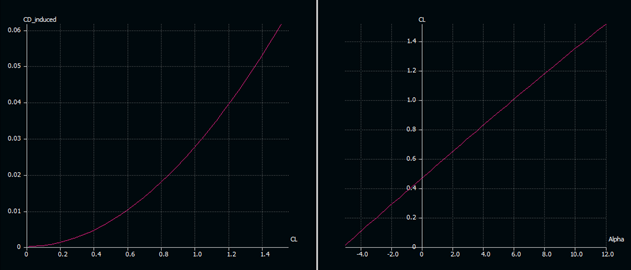
\includegraphics[width = 0.8\linewidth]{graphics/aero_simulation_chosen(CD).png}
 %   \caption{Drag coefficient induced by the trapezoidal wing}
%\end{figure}
%\begin{figure}[!ht]
   % \centering
    %	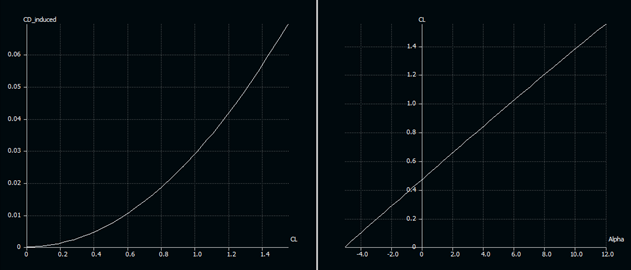
\includegraphics[width = 0.8\linewidth]{graphics/aero_simulation_elliptic(CD).png}
    %\caption{Drag coefficient induced by the trapezoidal wing}
%\end{figure}




\chapter{Structural Design}

By this point, most of the structural components of the aircraft have been defined. With this information, the project needs an approach to the internal structure design, to make assertions on the aircraft's ability to withstand different loads of various natures that might occur throughout a flight. This includes determining different values for forces and moments acting on the aircraft in order to make more informed decisions on the dimensions of the various structural components, and make sure the whole structure remains safe and sound for different situations.

\section{Structural Loads}

Studying the maximum loads for the aircraft will involve the analysis of the aerodynamic load factor, represented by the letter $n$. This factor represents the ratio of the lift and weight forces, and for cruise flight should ideally hold a value of $1$ as both forces equal each other.
\begin{gather}
    n = \frac{L}{W}
\end{gather}
This factor does however change through various flight conditions and manoeuvres, and its value for each of those conditions should be studied carefully as to not exceed dangerous values which might cause damage to the structure.

\subsection{The \vnd{} Diagram}

The aforementioned analysis done to the values of $n$ is graphically done using the \vnd{} diagram. This diagram correlates the value of airspeed with the value of $n$ throughout the entire flight and is useful for sketching limits for both speed and load factor and assists in visualising both their behaviour.

A good starting point for load factor limits can be found by using FAA's Federal Aviation Regulations, henceforth referred to as FAR, within part 23. These regulations contain typical standards for load factors, and their values were transcribed from \citetitle{corke} in table \ref{tab:far23}.
\begin{table}[ht]
    \centering
    \begin{tabular}{l c}\toprule
        Aircraft type       & Load factor               \\
        \midrule
        Normal aircraft     & $-1.25 \leq n \leq 3.1$   \\
        Utility aircraft    & $-1.8 \leq n \leq 4.4$    \\
        Acrobatic aircraft  & $-3.0 \leq n \leq 6.1$    \\
        \bottomrule
    \end{tabular}
    \caption{Maximum load factors based on FAR-23.}
    \label{tab:far23}
\end{table}

The chosen load factors correspond to the ones described for a normal aircraft. So,
\begin{gather}\label{eq:lf_far23}
    -1.25 \leq n \leq 3.1
\end{gather}
which gives us our first limits for the load factor.

Next we considered the load factor for extreme angles of attack. The sudden change in the angle of attack can cause an extra load on the structure which also needs to be correctly evaluated. The load factor for this situation is given by
\begin{gather}
    n = \frac{qC_L}{W/S}
\end{gather}
where $q$ is the dynamic pressure, which is dependent on the air density $\rho$ and the current airspeed $V$.
\begin{gather}
    q = \frac{\rho V^2}{2}
\end{gather}
With this information in hand, we can get the equation for the load factor with relation to airspeed.
\begin{align}\label{eq:lf_aoa}
    n = \frac{\rho V^2}{2}\cdot\frac{C_L}{W/S} = \frac{\rho SC_L}{2W}V^2
\end{align}

To continue building the \vnd{} diagram, we consider the maximum airspeed as the airspeed occurring during a dive, of which we take the value of $1.5$ times the cruise speed.
\begin{gather}
    V_{\text{dive}} = 1.5V_c
\end{gather}
With this all in mind, we sketched the diagram visible in figure \ref{fig:vn}. Visible are the load factor limits defined in equation \ref{eq:lf_far23} with data from table \ref{tab:far23} as horizontal lines both top and bottom, equation \ref{eq:lf_aoa} and its symmetrical as both lines starting at $V = \SI{0}{\meter\per\second}$ and the limit dive speed $V_{\text{dive}}$ at the very right of the graph. The final diagonal stretch is used to enclose the diagram.

\begin{figure}[ht]
    \centering
    \begin{tikzpicture}
    \begin{axis}
            [width = 0.9\linewidth,
            legend cell align=left,
            legend style={at={(0.5,-0.15)},anchor=north},
            grid = both,
            xmin = 0, xmax = 48,
            ymin = -1.6, ymax = 3.3,
            xlabel = {Velocity $V$ $[\si{\meter\per\second}]$},
            ylabel = {Load factor $n$},
            cycle list = {red,blue,cyan,teal,orange,purple,violet,brown,darkgray,magenta},]
        \addplot +[domain = 0:40.723] {0.001869*x^2}; \addlegendentry{High angle of attack};
        \addplot +[domain = 0:25.863] {-0.001869*x^2}; \addlegendentry{High angle of attack};
        \addplot coordinates {(40.723,3.1)(45,3.1)}; \addlegendentry{Maximum load factor ($n = 3.1$)};
        \addplot coordinates {(25.863,-1.25)(30,-1.25)}; \addlegendentry{Maximum negative load factor ($n = -1.25$)};
        \addplot coordinates {(45,0)(45,3.1)}; \addlegendentry{Dive speed ($V = \SI{45}{\meter\per\second}$)};
        \addplot coordinates {(45,0)(30,-1.25)};
    \end{axis}
\end{tikzpicture}
    \caption{\vnd{} diagram.}
    \label{fig:vn}
\end{figure}

\subsection{Gust loads}

While the initial \vnd{} diagram is concluded, \textit{gust loads} are yet to be considered. Gust loads are sudden and momentary aerodynamic loads caused by atmospheric turbulence that affect the aircraft structure and need to be accounted for in an aerodynamic load analysis.

The effect of a gust load is often noted as a variation of the aerodynamic load factor $\Delta n$. This variation can be either positive or negative, and both varieties need to be accounted for in our analysis.

The gust load also causes a slight variation in the airspeed of the aircraft. If we decompose the speed as in figure \ref{fig:v_gustloads}, considering we use $V$ for airspeed, $u$ will be the normal speed and $v$ the variation in the speed in the velocity axis. This variation is usually negated due to it being that much less than the travel velocity.
\begin{figure}[ht]
    \centering
    \begin{tikzpicture}
        \coordinate (ref) at (0,0);
        \path [draw, -{Stealth[]}] (ref) -- node [auto,swap] {$V + v$} (3,0);
        \path [draw, -{Stealth[]}] (ref) -- (3,1);
        \path [draw, -{Stealth[]}] (3,0) -- node [auto,swap] {$u$} (3,1);
    \end{tikzpicture}
    \caption{Decomposing the velocity components for gust loads.}
    \label{fig:v_gustloads}
\end{figure}
With this information, assuming the original normal velocity $u$ is zero before a gust, the value of $u$ after a gust can be determined by the gust velocity $\hat{u}$ and the response of the aircraft, which will be calculated further ahead.

Using the decomposition from figure \ref{fig:v_gustloads} we can determine the variation of the aerodynamic load $\Delta n$.
\begin{gather}\label{eq:gl_dn}
    \Delta n = \frac{\rho uVSC_{L_\alpha}}{2W}
\end{gather}
As we mentioned, the value of $u$ is purely dependent on the gust velocity, but also the aircraft's response to each gust. This response is dependent on the aircraft's characteristics, but also the gust's frequency. The aircraft's response to this frequency can be summarised using the aircraft's mass ratio, represented by the variable $\mu$.
\begin{gather}\label{eq:gl_mu}
    \mu = \frac{2W/S}{\rho g\bar{c}C_{L_\alpha}}
\end{gather}
We can use the mass ratio to characterise the effect of the gust speed on the aircraft's normal velocity $u$, but not directly. We define the aircraft's response coefficient $K$, which correlates the values of $u$, the aircraft's new normal velocity, with the speed of the gust, $\hat{u}$.
\begin{gather}\label{eq:gl_uhat}
    u = K\hat{u}
\end{gather}
This value of $K$ can be related with the value of $\mu$ directly, but is dependent on whether the current flight condition is subsonic or supersonic. For this project, we only considered the subsonic situation, which can be described as follows.
\begin{gather}\label{eq:gl_k}
    K = \frac{0.88\mu}{5.3 + \mu}
\end{gather}
And so, with equations \ref{eq:gl_dn}, \ref{eq:gl_mu}, \ref{eq:gl_uhat}, and \ref{eq:gl_k}, we can obtain the relation between the aerodynamic load and the gust speed.

The FAA has established some gust velocities to be used for calculations for this type of analysis. These velocities are dependent on the flight altitude, but are the same for every altitude below $\num[group-separator = \text{~}]{20000}\,ft$. In this case, the gust velocities are the ones found in table \ref{tab:gustvelocities}.
\begin{table}[ht]
    \centering
    {\sisetup{range-phrase = --, group-separator = \text{~}}
    \begin{tabular}{l c c}\toprule
        Flight condition        & Altitude range ($ft$) & $\hat{u}$ ($ft/s$)    \\
        \midrule
        High angle of attack    & \numrange{0}{20000}   & $66$                  \\
        Level flight            & \numrange{0}{20000}   & $50$                  \\
        Dive condition          & \numrange{0}{20000}   & $25$                  \\
        \bottomrule
    \end{tabular}
    }
    \caption{Different values of gust velocities to be tested \cite{corke}.}
    \label{tab:gustvelocities}
\end{table}

With these values, we plotted the lines corresponding to the equation
\begin{gather}
    n = 1 \pm \Delta n
\end{gather}
with the values for $\Delta n$ obtained using equation \ref{eq:gl_dn}. These plots can be found in figure \ref{fig:vn_gusts}.
\begin{figure}[ht]
    \centering
    \begin{tikzpicture}
    \begin{axis}
            [width = 0.9\linewidth,
            legend cell align=left,
            legend style={at={(0.5,-0.15)},anchor=north},
            grid = both,
            xmin = 0, xmax = 48,
            ymin = -1.6, ymax = 3.3,
            xlabel = {Velocity $V$ $[\si{\meter\per\second}]$},
            ylabel = {Load factor $n$},
            cycle list = {red,blue,cyan,teal,orange,purple,violet,brown,darkgray,magenta},]
        \addplot +[domain = 0:40.723,forget plot] {0.001869*x^2};
        \addplot +[domain = 0:25.863,forget plot] {-0.001869*x^2};
        \addplot +[forget plot] coordinates {(40.723,3.1)(45,3.1)};
        \addplot +[forget plot] coordinates {(25.863,-1.25)(30,-1.25)};
        \addplot +[forget plot] coordinates {(45,0)(45,3.1)};
        \addplot +[forget plot] coordinates {(45,0)(30,-1.25)};
        \addplot +[dashed, domain = 0:50] {1 + 0.0959042377206059*x}; \addlegendentry{Wind gust of $66\,ft/s$};
        \addplot +[dashed, domain = 0:50] {1 + 0.0726547255459136*x}; \addlegendentry{Wind gust of $50\,ft/s$};
        \addplot +[dashed, domain = 0:50] {1 + 0.0363273627729568*x}; \addlegendentry{Wind gust of $25\,ft/s$};
        \addplot +[dashed, domain = 0:50] {1 - 0.0363273627729568*x}; \addlegendentry{Wind gust of $25\,ft/s$};
        \addplot +[dashed, domain = 0:50] {1 - 0.0726547255459136*x}; \addlegendentry{Wind gust of $50\,ft/s$};
        \addplot +[dashed, domain = 0:50] {1 - 0.0959042377206059*x}; \addlegendentry{Wind gust of $66\,ft/s$};
    \end{axis}
\end{tikzpicture}
    \caption[\vnd{} diagram with gust speeds.]{\vnd{} diagram with gusts sketched for different wind gust speeds adapted from table 10.3 from page 213 of \citetitle{corke} \cite{corke}.}
    \label{fig:vn_gusts}
\end{figure}

\subsection{Design Load Factor}

Using the \vnd{} diagrams sketched previously, we can obtain a maximum value for the load factor. This value is equal to the maximum value of the manoeuvring load factors visible in figure \ref{fig:vn} and the added load factor due to gusts visible in figure \ref{fig:vn_gusts}. This factor is usually titled the limit load factor.

This factor, however, is usually multiplied by a safety factor $SF$ to provide a margin of safety for the structure's performance. The most commonly used value for this safety factor is $1.5$, mainly due to historical reasons, and is the one we will apply to our project as well.

This final factor is called the design load factor and can be expressed as in equation \ref{eq:lf_design}.
\begin{gather}\label{eq:lf_design}
    n_{\text{design}} = 1.5\left(n_{max} + \Delta n\right)
\end{gather}

Using the data implemented throughout the project, we arrive at a design load factor of
\begin{gather}
    1.5\times(3.1796 + 3.1) = 9.4194
\end{gather}

\subsection{Wing Load Distribution}

In this section an analysis of the wing shear force and bending moment of the wing section is made. The lift distribution and the bending moment of the projected wing are shown in figures \ref{fig:liftdistribution} and \ref{fig:momentdistribution}, respectively.

\begin{figure}[!ht]
    \centering
    \includegraphics[width = 0.8\linewidth]{bending_moment.png}
    \caption{Bending moment distribution through the wing, obtained from XFLR5.}
    \label{fig:momentdistribution}
\end{figure}

\begin{figure}[!ht]
    \centering
    \includegraphics[width = 0.8\linewidth]{lift_distribution.png}
    \caption{Lift coefficient distribution through the wing, obtained from XFLR5.}
    \label{fig:liftdistribution}
\end{figure}

Noticing that not considering the safety factor applied to the maximum load factor
\begin{gather}
    n_{max}=6.3=\frac{L}{W}
\end{gather}
So, the maximum lift can be determined as
\begin{gather}
    L = 2067.9\,N
\end{gather}
Analysing the lift distribution of the main wing, we can notice a trapezoidal shape to it, and using this tendency, the respective trapezoidal lift distribution is assumed. Further loads applied to the wing are its weight (assumed to be $2\,kg$ distributed along the semi-span) and the punctual weight referring to the booms supporting the VTOL system and the tail, whose weight is assumed to be $2.457\,kg$. The final force distribution, shear force and bending moments along the wing are shown in figures \ref{fig:loaddistribution}, \ref{fig:shear forces}, \ref{fig:bending moment}, and \ref{fig:Reactions}, where it is also assumed that the wing acts like a cantilevered beam.

\begin{figure}[!ht]
    \centering
    \includegraphics[width = 0.9\linewidth]{graphics/Loads_distribution.png}
    \caption{Approximated load distribution. Weight summed with the lift distribution}
    \label{fig:loaddistribution}
\end{figure}

\begin{figure}[!ht]
    \centering
    \includegraphics[width = 0.9\linewidth]{graphics/Shear_force.png}
    %\input{graphics/tikz/shearforce.tikz}
    \caption{Shear force}
    \label{fig:shear forces}
\end{figure}

\begin{figure}[!ht]
    \centering
    \includegraphics[width = 0.9\linewidth]{graphics/bending_moment_f.png}
    %\input{graphics/tikz/bendmoment.tikz}
    \caption{Bending moment}
    \label{fig:bending moment}
\end{figure}

\begin{figure}[!ht]
    \centering
    \includegraphics[width = 0.9\linewidth]{graphics/reactions.png}
    \caption{Reactions}
    \label{fig:Reactions}
\end{figure}

It is relevant to notice that the lift distribution considered is a result from the XFLR results of the joint wing and fuselage configuration, so there is a decrease in lift closer to the root spans.

As shown in the aforementioned figures, these results have a high order of magnitude, but the load factor considered is also high. The relevance of these results lie on the need of construct a sturdy structure to withstand high levels of loads, but the detail depth will only be considered in a later stage of development, not included in this project and subsequent report.

\section{Material Selection}

The next step in the conception process is to choose a suitable material for the aircraft. Due to the considered mission, a material with a low magnetic interference is preferred. Furthermore, the material needs a high resistance to shear forces and bending moments, specially regarding the wing. The material density has to be as low as possible to keep the weight equally low. With these requirements taken into account a composite material was selected for the aircraft main structural components by analysing table \ref{tab:compositematerials}.
\begin{table}[!ht]
    \centering
    \includegraphics[width = 0.9\linewidth, trim = {0 3mm 0 15mm}, clip]{graphics/Propriedades_Material.png}
    \caption{Composite materials (table 10.9 from \citetitle{corke} \cite{corke}).}
    \label{tab:compositematerials}
\end{table}

A graphite-epoxy with a $60\%$ fibre volume was selected, due to its low density and good rigidity modulus. Furthermore, this is a material available in the CAD software used, which eases the weight and centre of gravity position calculation of the whole aircraft. This material has a density of \SI{1.6e-6}{\kilogram\per\milli\meter\cubed}.

An important detail that has to be taken into account is the magnetic interference of this material. The nose of the aircraft has to be made of a material that does not reflect or absorb electromagnetic radiation. As graphite-epoxy has a significant magnetic interference. Taken inspiration from the current commercial aircraft, mainly in their radome,  E- fibre glass is assigned to the frontal area of the fuselage covering the MAD sensor. For simplistic reasons, a density similar to that of the graphite-epoxy material was assumed. 

Based on historical values, a fuselage with $1\,mm$ and $2.5\,mm$ of skin thickness for the wing and tail were assigned. Regarding the booms, a more significant skin thickness of $4\,mm$ was selected, because this is a main structural element of the design, having to be hollow in order to pass all the cabling needed for the VTOL engines.

The final component weights are shown in chapter \ref{chap:Stability analysis}. As a concluding remark, it is relevant to highlight the need to proceed with further structural analysis and layout the structural elements inside the wings, tail, and fuselage. 

\chapter{Avionics}

Avionics are the electronic systems used on an aircraft and play a crucial role on the final weight, design and cost of an unmanned aerial vehicle. The avionics comprise the onboard hardware and software responsible for guidance, navigation and control of the UAV, the payload and its data acquisition and processing systems and the modules employed for communication with the ground.

In this project it will be analyzed in detail all the electronic components necessary for the UAV operation and it will be selected the most convenient commercial solutions available in the market. In the end of this section a schematic of the avionics systems will be presented as well as an estimation of their total weight and cost.

\section{Autonomous Operations}

Considering the range and the goals of the UAV mission, an autonomous onboard control system will be required. It'll have the following main functions:
\begin{description}
	\item[Navigation] The UAV will need to carry out a pre-programmed route, so it'll be mandatory to know its location. Therefore, the control system should estimate the vehicle's position, attitude and velocity through the fusion of the data obtained from the Inertial Measurement Unit, the GPS receiver, the Barometric altimeter and the Airspeed Sensor.
	\item[Guidance] The control system will have to compute the changes in position, velocity, attitude, and rotation rates required to follow the mission's trajectory based on the UAV actual state of motion. Guidance's and Navigation's calculations complexity will determine the onboard processing power required.
	\item[Control] The control system must send corrective signals to the Electronic Speed Controller and to the flight control surfaces' actuators to keep the UAV on its predefined path.
	\item[Communication] The control system will be able to receive commands from a ground station and send, through a data link module and its antenna, information of the UAV's payload, position, attitude, air data and fuel and battery status.
	\item[Sense and Avoid] With airspace becoming increasingly crowded and UAVs becoming more popular, a reliable sense and avoid system is convenient, especially in autonomous operations like this one. Therefore, the control system should be compatible with a collision avoidance technology and should, using its information, autonomously prevent a collision.
\end{description}

Summarizing, the software of the selected intelligent onboard flight control system must accept and process data from the UAV's sensors, compute and compare the state of the vehicle (position, orientation and velocity) with the one intended in the mission profile and make appropriate corrections, while reacting to unforeseen events and sending real time data to a ground station.

\section{Autopilot and Sensors}

The easiest way to achieve UAV autonomous operations is to implement in our design one of the open source or commercial onboard autopilot solutions available in the market. An autopilot is a modular system consisting of a microcontroller unit and various sensors and servo actuators communicating through independent buses for high reliability. The data collected by the sensors is processed and evaluated by an algorithm that determines the electric signals to be applied to the actuators. A sophisticated autopilot is composed by:
\begin{description}
	\item[Microcontroller Unit] This component is the brain of the UAV. It's connected and receives the signals of all the sensors and modules and its processor runs the code needed for estimating the vehicle's attitude, velocity and position (Navigation), computes the path based on the actual vehicle status (Guidance) and sends the corrective actions to the actuators (Control)
	\item[Inertial Measurement Unit] Electronic device composed by a combination of 3-axis accelerometers, gyroscopes and magnetometers that measures the accelerations, the rotational velocities and the magnetic field components along its axes. The data reported by the IMU is fed into the processor which calculates UAV's attitude, velocity and position. With this information the flight control system is able to determine how stable is the vehicle. 
	\item[GNSS Sensor] This unit uses the signals sent by one or more satellite constellations to estimate the absolute position and velocity of the UAV. An autopilot can either have an onboard GNSS module or one which is connected to it via a cable. The GNSSS antenna should not be confused with the GNSS chip itself and can look like a small black box or a normal duck antenna. In order to get an accurate GNSS lock, the GNSS chip should receive data from multiple satellites. 
	\item[Barometric Altimeter] This module measures the barometric pressure and estimates the elevation above mean sea level based on the standard atmospheric model. The autopilot takes input from both the altimeter and GNSS module to calculate a more accurate estimation of the UAV's altitude. It's important to have the barometer covered to diminish the effects of wind over the chip. 
	\item[Airspeed Sensor] Air speed measurement is of major importance for VTOLs and fixed wing UAVs. It helps the autopilot in windy conditions, slow flight and autonomous landings. This unit is linked to a pitot tube, that measures the dynamic pressure of the air flow, and a pressure sensor that measures the static pressure of the air. 
	\item[Distance Sensor] This module measures the distance between the sensor and any object within its working range and can be used for detecting obstacles. A distance sensor might be based on sonar or LIDAR technology. This unit provides obstacle avoidance functionality for the autopilot.
\end{description}
Although there are several complete auto pilots on the market compatible with a ground control station and with functionalities like autonomous waypoint navigation flight, only a small percentage of them incorporates VTOL capabilities. Within these solutions we will study the implementation of two of them, an open source one, ArduPilot, that is cheaper, extremely customizable and has a large support community and a commercial one, MicroPilot, that is more reliable and has more sophisticated and certified high-quality components.


\section{Micropilot}

For this project, the method of flight control is of extreme importance due to the lack of an onboard human pilot to maneuver the aircraft. Therefore, a mechanism for stabilizing and controlling the aircraft must be selected. Although the selection is not crucial for the study of the project's objectives, the method selection was made with the remaining characteristics in mind to ensure it would fit the objectives as best as it could, or at least not to interfere with them.

The basic requirements for integration within our project were mainly native support for VTOL characteristics, which proved to be the most challenging to find a proper solution for, and support for both UAV and RPV flight modes for trajectory control. \par
\vspace{0.25cm}
After discussing a number of options for an off-the-shelf commercial autopilot, we chose the MicroPilot \micropilot{} VTOL autopilot, by Winnipeg-based Canadian manufacturers MicroPilot. One of the major deciding factors was the native implementation of fixed-wing aircraft control with integrated VTOL capabilities, support for both UAV and RPV flight modes, and the inclusion of a ground station with proprietary user-friendly software, but many more features have turned the decision towards MicroPilot's offering. Among the features listed, a couple more have caught our attention:
\begin{itemize}
	\item \textit{SWIL}\footnotemark{} simulator for operator training in RPV mode;
	\item Integrated gyros, accelerometers, pressure altimeter and airspeed sensors, and GPS sensor;
	\item Waypoint-based UAV navigation, programmable via MicroPilot's \textit{Horizon} software suite;
	\item Support for dead-reckoning navigation.
\end{itemize}
\footnotetext{\textit{Software-In-The-Loop}, a simulation type which simulates an environment for the autopilot to run as if it were running in a real flight. This requires a mathematical model of the aircraft's aerodynamic and thrust model for the simulation to make any calculations.}

The goal for control within our project will be to control the aircraft remotely manually, also referred to as RPV flight mode.
\newpage
\section{Ardupilot}

The ArduPilot will be our alternative solution, for situations where the price is more important than the weight and processing power of the autopilot. \par

The ArduPilot board needs to be supplied by a power source. This is achieved by using the 3DR Power Module (Figure \ref{fig:ardupilot_powermodule}). This can be connected to the hover battery of the UAV while also supplying the ArduPilot board with the required power. The Power Module also allows the monitoring of the battery voltage level in the Mission Planner. The GPS and Compass data are provided by the 3DR GPS Module (Figure \ref{fig:ardupilot_gpsmodule}). \par


\begin{figure}[h]
  \centering
  \begin{minipage}[t]{0.5\linewidth}
    \centering
    \includegraphics[width=\textwidth]{graphics/AVIONICS/ardupilot1.png}
    \caption{3DR Power Module}
    \label{fig:ardupilot_powermodule}
  \end{minipage}%
  \begin{minipage}[t]{0.5\linewidth}
    \centering
    \includegraphics[width=\textwidth]{graphics/AVIONICS/ardupilot2.png}
    \caption{3DR GPS Module}
    \label{fig:ardupilot_gpsmodule}
  \end{minipage}
\end{figure}

The airspeed sensor (Figure \ref{fig:ardupilot_AirspeedSensor}), has a pressure sensor and a pitot tube. It measures the airspeed which helps the autopilot in windy conditions, slow flight and autonomous landings. The top tube of the sensor measures the dynamic pressure of the air flow that passes through the pitot tube and the bottom tube measures the static pressure of the air. The Sonar Sensor (Figure \ref{fig:ardupilot_SonarSensor}) provides obstacle avoidance functionality to the ArduPilot. It measures the distance between the sensor and an obstacle in front of it.

\begin{figure}[h]
  \centering
  \begin{minipage}[t]{0.5\linewidth}
    \centering
    \includegraphics[width=\textwidth]{graphics/AVIONICS/ardupilot3.png}
    \caption{Airspeed Sensor}
    \label{fig:ardupilot_AirspeedSensor}
  \end{minipage}%
  \begin{minipage}[t]{0.5\linewidth}
    \centering
    \includegraphics[width=\textwidth]{graphics/AVIONICS/ardupilot4.png}
    \caption{Sonar Sensor}
    \label{fig:ardupilot_SonarSensor}
  \end{minipage}
\end{figure}

Ground Control Station: Ardupilot provides an open source software called Mission Planner. Mission Planner provides a user-friendly interface that allows quick interactions between the ground controller and the aircraft. The ground controller can monitor several flight parameters, such as airspeed, altitude, heading, among others and can even see the current position of the vehicle in a map.

\begin{figure}[ht]
    \centering
    \includegraphics[width=\textwidth]{graphics/AVIONICS/ardupilot5.jpg}
    \caption{Mission Planner Interface}
    \label{fig:ardupilotplannerinterface}
\end{figure}

\newpage
\vspace{1cm}
The final connections between the sensors and the microcontroller are presented in Figure \ref{fig:ardupilotconnections}.
\vspace{1cm}
\begin{figure}[ht]
    \centering
    \includegraphics[width=\textwidth]{graphics/AVIONICS/ardupilot6.png}
    \caption{Connections to perform between the components.}
    \label{fig:ardupilotconnections}
\end{figure}


\newpage

\section{Electronic Speed Controllers}
An Electronic Speed Controller (ESC) enables the control system to send corrective signals to the electric motors to keep the UAV on its predefined path during the Vertical Take-Offs and Landings. \par
Different types of speed controls are required for brushed DC motors and brushless DC motors. A brushed motor can have its speed controlled by varying the voltage on its armature. A brushless motor requires a different operating principle. The speed of the motor is varied by adjusting the timing of pulses of current delivered to the several windings of the motor. Therefore, we must take into account when choosing the commercial electronic speed controller, that our rotors are brushless. \par
Fortunately, KDE Direct (the brand of our electric motors and our propellers) also sells electronic speed controllers. So, we just have to choose the proper ESC for our set of multi-rotors plus propeller blades - which corresponds to the $KDEXF-UAS95$HVC product. \par
\begin{figure}[ht]
    \centering
    \includegraphics[width=0.5\textwidth]{graphics/AVIONICS/b.jpg}
    \caption{KDEXF-UAS$95$HVC Electronic Speed Controller}
    \label{fig:kdespeedcontroler}
\end{figure}

The main specifications of this Electronic Speed Controller are the following:
\begin{itemize}
    \item Programming: Proprietary Algorithm, $600Hz$ Refresh, Dynamic Advance Timing
    \item Maximum Peak Current: $165$ A ($5s$)
    \item Maximum Peak Power: $7,325$ W ($5s$)
    \item Maximum Efficiency:	> $98\%$
    \item Voltage Range	:$11.1$ V ($3S$ LiPo) to $52.2$ V ($12S$ LiHV).
    \item ESC Size: $37\ mm\ (W) \times 82$ mm (L)
    \item ESC Weight: $78$ g ($114$ g with Wires/Bullets)
\end{itemize}

\begin{figure}[ht]
    \centering
    \includegraphics[width=0.9\textwidth]{graphics/AVIONICS/a.png}
    \caption{Dimensions of the  KDEXF-UAS$95$HVC Electronic Speed Controller}
    \label{fig:kdespeedcontrolerdim}
\end{figure}

\section{Actuators}
An actuator enables the control system to send corrective signals to the flight control surfaces’ in order to keep the UAV on its predefined path. An actuator requires a control signal and a source of energy. When it receives a control signal, an actuator responds by converting the signal's energy into mechanical motion. \par
Since our autopilot will be the MP$2128^{\text{HELI}2} $ model of the MicroPilot company, it is advantageous to use Volz actuators because the MP$2128^{\text{HELI}2} $ supports Volz actuators protocols. \par

\begin{figure}[ht]
    \centering
    \includegraphics[width=0.3\textwidth]{graphics/AVIONICS/actuators.png}
    \caption{Volz’s DA-$15$-T Throttle Actuator}
    \label{fig:volzthrotactuator}
\end{figure}

This throttle servo is a compact fly-by-wire actuator for direct installation on the throttle valve shaft of a combustion engine. That eliminates the need for the rudder linkage and bowden cables, shortens the installation time and minimizes the installation space and overall weight.

\begin{figure}[ht]
    \centering
    \includegraphics[width=0.3\textwidth]{graphics/AVIONICS/servoactuators.jpg}
    \caption{Volz’s DA $10-05-42$ Servo Actuator.}
    \label{fig:volzservoactuator}
\end{figure}

This will be the servo actuator used in the ailerons control system. It’s a fully programmable, low profile micro actuator with all steel gear train. Thanks to its reduced size, it fits into smallest airfoil cross-sections.\par 
Both actuators comprise a DC motor, gear train and control electronics governed by microprocessors with integrated position feedback.

\chapter{Magnetic Interference} 
Mounting magnetometers on aircraft has always provided engineers a significant challenge. Being fundamental to flight, propulsion and flight controls systems all carry significant magnetic properties. Gas combustion engines, DC brushless motors and flight control servos all contain strong permanent magnets, electromagnetic windings, and ferromagnetic material. Since these systems cannot be removed it is necessary to mitigate their effects on magnetometer payloads, and ultimately the detection capabilities of the aircraft. Furthermore, material with strong magnetic properties can induce magnetization in other materials. This is an important consideration regarding assembly and tooling. Strong tool control and magnetic discipline are required as to prevent unintentional magnetic contamination. \par
In this section, we will summarize the magnetic noise sources onboard of the vehicle, recurring to the bibliographic reference \cite{mag_thesis}, and we will present the results of the magnetic interference measurements done in the Excel file.  \par
In the Excel file we will evaluate and quantify the magnetic interference originated from the following four sources:\par
\begin{itemize}
    \item \textbf{Permanent Magnets and Hard Ferromagnetic Materials}: The most well-known sources of static onboard vehicle noise come from the propulsion and flight control servos when inactive. Combustion engines, electric motor/generators and servos all contain permanent magnets and ferromagnets that contribute to the vehicles magnetic noise level. Furthermore, it is common to use a magnetic safety shunt to ensure the vehicle’s propulsion or electrical system remains inactive until deliberately removed. In our project and in our calculations, we will consider the permanent magnets and hard ferromagnetic materials present in the following components:
    \begin{itemize}
        \item Flight Control Servos;
        \item Brushless Motors;
        \item Combustion Engine;
        \item Magnetic Safety Switch.
    \end{itemize}
    \item \textbf{DC Electromagnets}: Electrical currents induce magnetic fields. Electromagnets, in general, can be considered weak permanent magnets. The obvious source of DC electromagnetic noise on aircraft is the extensive amount of electrical wires. Electrical wires typically reach all regions of the vehicle but remain most concentrated within avionics or sensor bays. Further sources of noise could be found near the battery compartments. \par As DC electrical sources, batteries can also produce static magnetic noise from a parasitic current draw, even when the connected components are powered-off. Moreover, any other conductive material that comes into contact current-carrying sources will also become a source of static magnetic noise. In our UAV we can find the DC Electromagnets in the following components:
    \begin{itemize}
        \item Conductors/Electrical Wires that carry or touch DC current;
        \item Batteries;
        \item Sensors;
        \item Avionics;
        \item Electronic Speed Controllers. 
    \end{itemize}
    \item \textbf{Changing Electric Flux}: A transient magnetic field is a magnetic field source that varies with time. Transient magnetic sources include changes in electric and magnetic fluxes. This topic only considers magnetic sources produced by changing electric flux. Ampère-Maxwell law states that a constant current or changing electric flux induces a magnetic field. Given the large amount of AC-powered or load-dependent electronics within a vehicle, many sources of transient magnetic noise can be identified:
    \begin{itemize}
        \item Autopilot;
        \item Electronic Speed Controllers;
        \item RF Transmitters;
        \item Throttle servos;
        \item Flight Controls;
        \item Inverters and Transformer Rectifier Units (TRU)
        \item Avionics and Sensors;
        \item All the other components that carry AC current.
    \end{itemize}
    \item \textbf{Rotating Propulsive Components}: Variable AC currents produce variable transient magnetic fields. Within the rigid and flexible vehicle frames of reference, there are propulsive components that rotate internally which produce significant transient magnetic noise. Generally, electric engines have been found to produce more magnetic noise than combustion engines in airborne UAV magnetometry applications. \par DC brushless motors are the most common for UAV propulsion. The motor has a permanent magnet rotor surrounding a stator composed of a series of coil-pairs which act as electromagnets. When DC voltage is passed through the coil-pairs, a magnetic field is produced which interacts with the PM rotor. The rotor begins to rotate away from the coil-pairs as they are selectively sequenced to induce rotary motion. The magnetic noise consequences of this rotary motion produce a significant amount of changing magnetic flux noise. The changing magnetic flux has the effect of inducing currents in surrounding conductive surfaces, which then produce their own magnetic fields.\par
    Similarly, combustion engines are also significant magnetic noise sources. It is common that crankshaft, pistons, cam valve pins and connecting rods are made of high ferritic steels. The rotating propulsive components that can be found in our UAV are:
    \begin{itemize}
        \item DC Brushless Motors (We will not consider the magnetic interference caused by the rotation of these components because they’ll be inactive during the magnetic anomaly detection, i.e. during cruise. We’ll only consider the interference caused by the permanent magnets and ferromagnetic material of these components)
        \item Combustion Engine;
        \item Rotating Servos.
    \end{itemize}
\end{itemize}

Since we already identified the main sources of magnetic interference aboard our drone, we will present the results obtained in the excel file. After the insertion of the location of the magnetic sensor and of each of the components on board the aircraft, according to the coordinate system shown in figure x, we got a magnetic interference on the sensor of \textbf{1.938nT}. 

\begin{figure} [ht]
    \centering
    \includegraphics{graphics/AVIONICS/magnetic.png}
    \caption{Coordinate system used in the magnetic interference analysis.}
    \label{fig:magcoord}
\end{figure}

This value is \textbf{less than 2nT} expressed in the requirements. In order to reach this value, it was necessary to carefully design the length of the fuselage and the distribution of each of the components in it. The elements that most cause magnetic interference in the sensor were the combustion engine (which is active during the magnetic anomaly detection) and the permanent magnets and ferromagnetic material present in the brushless motors that cause magnetic noise even in cruise, when the brushless motors are inactive. \par
We can then conclude that the length of the fuselage was strongly influenced by the magnetic analysis because it corresponded to the minimum length that ensured that the brushless motors, the combustion engine and the other elements there stored did not produce high levels of noise for the sensor.



\chapter{Stability analysis}\label{chap:Stability analysis}

\section{Static stability}
In the design of a new aircraft, it is important that it is statically stable during flight. Static stability is related to the aircraft's ability to return to its equilibrium position after it has been disturbed and without pilot or autopilot intervention. On the other hand it is important to note that excess stability can have negative effects on aircraft maneuverability and performance. Thus, it was intended that the projected aircraft be stable but without compromising its performance and maneuverability, in order to ensure that it is capable of accomplishing its mission. 

Since the stability of an aircraft is dependent on the $3$ directions of movement. It can be divided into longitudinal stability, relative to the movements in which the aircraft remains in the plane of symmetry, lateral stability that covers lateral movements, and directional stability that covers directional movements. 

A simple way to evaluate its static stability is to obtain the distance between the center of gravity and the aerodynamic center. However, the center of gravity generally varies in position during flight for various reasons, for example because of fuel consumption or cargo release. This variation of C.G. may change the stability behavior of the aircraft. Thus it is important during the design phase to place the components responsible for this variation close to the center of gravity to minimize their effects. For this reason and because of the only component that varies its mass during flight, the fuel tank of the projected aircraft was placed near the center of gravity.

Weights and centers of gravity of the components of the aircraft (fuel full and fuel empty):

\begin{table}[ht]
    \centering
   \begin{tabular}{l C C C}\toprule
       Components                   &  \text{Weights [kg]}  & \text{Position [mm]}   &  y\times m [mm\times kg] \\
       \midrule
       Motor                       & {1,2}          & {1065.23}    &  {1278.27}\\
       Fuselage                     & {5.593}        & {120.729}    &  {675.237}\\ 
       Wing+tail                   & {7.694}        & {610.237}    &  {4696.2}\\ 
       Sensor                       & {1.1}          & {-552.98}    &  {-608.28}\\
       Fuel tank                   & {4}            & {-123.9}     &  {-495.6}\\
       Batteries                    & {2.652}        & {183.099}    &  {485,579}\\
       Avionics                     & {1.5}          & {354.599}    &  {531.899}\\
       Payload                      & {8.5}          & {-332.4}     &  {-2825.4}\\
       Electric motors (VTOL)        &  1.22          & 116          & 202.52 \\   
       \bottomrule
    \end{tabular}
   \caption{Weights and centers of gravity of components with the fuel tank full}
    \label{tab:cg of components full}
\end{table}


\begin{table}[ht]
    \centering
    \begin{tabular}{l C C C}\toprule
    Components                   &  \text{Weights}  & \text{Position}   &  y\times m \\
    \midrule
    Motor                        &  1.2             & 1065.23           &  1278.27\\
    Fuselage                     &  5.593           & 120.729           &  675.237\\ 
    Wing+tail                    &  7.694           & 610.237           &  4696.2\\ 
    Sensor                       &  1.1             & -552.98           & -608.28\\
    Fuel tank                    &  0.5             & -123.9            & -61.951\\
    Batteries                    &  2.652           & 183.0992          &  485.5791\\
    Avionics                     &  1.5             & 354.599           &  531.8985\\
    Payload                      &  8.5             & -332.4            & -2825.4\\
    Electric motors(VTOL)        &  1.22            & 116               & 202.52 \\      
    \bottomrule
    \end{tabular}
    \caption{Weights and centers of gravity of components with the fuel tank empty}
  \label{tab:cg of components empty}
\end{table}
\begin{equation}
    \overline{Y} = \frac{\sum{Y\cdot m}}{\sum{m}}
    \label{eq. determination center of gravity}
\end{equation}
The center of gravity is calculated using the equation \ref{eq. determination center of gravity}. Notice that all these coordinates are related with the origin of the cad model, which is placed 200mm ahead of the wing´s leading edge. 

The values for the center of gravity were obtained:
\begin{itemize}
\item Aircraft with full fuel tank: $119.409\,mm$
\item Aircraft with empty fuel tank: $149.04\,mm$
\end{itemize}
 
 The MTOW weight is also shown to be less that 35Kg, more specificaly 33.796Kg
\begin{figure}[!ht]
    \centering
    	\includegraphics[width = 0.55\linewidth]{graphics/image_cg_position.png}
    \caption{Center of gravity on the aircraft}
    \label{fig:center of gravity on the aircraft}
\end{figure}

\subsection{Longitudinal stability}
The requirement to be statically stable in longitudinal movement, the center of gravity must be ahead of the neutral point (is the point where the moment coefficient about the center of gravity does not vary with the angle of attack). In other words, the static stability in longitudinal motion requires that the derivative:

\begin{equation}
   C_{M_{\alpha}} = \dfrac{d C_{M_{cg}}}{d 
   \alpha} < 0 
    \label{eq. long_moment coefficient}
\end{equation}

\begin{equation}
   SM = \dfrac{x_{np}-x_{cg}}{\overline c} > 0 
    \label{Static margin}
\end{equation}

Using the stability analysis of program XFLR5, the neutral points were determined:
\begin{itemize}
\item aircraft with full fuel tank: 658,94 $mm$
\item aircraft with empty fuel tank: 659,59 $mm$
\end{itemize}

Using the expression, the static margin obtained were 2.09 (full tank) and 1.98 (empty tank). It is thus concluded that in both cases the aircraft is longitudinally stable. It is important to note that the position of the neutral point remains in the same position with the variation of the fuel.On the other hand, as can be seen in the table \ref{tab:long_derivatives}, Cma is negative (stable), however it is outside the limit of the values that would be more appropriate (-1.5< Cma <-0.16). That may lead to a reduction in aircraft maneuverability.

\subsection{Lateral stability}
The requirement for lateral static stability is that the right wing tip should rotate up to counter a positive sideslip angle $\beta$. Therefore the static stability in lateral motion requires that the derivative:

\begin{equation}
   C_{L_{\beta}} = \dfrac{dC_{L_\beta}}{d\beta} < 0 
    \label{eq. lat_moment coefficient}
\end{equation}

However, because it is difficult to estimate the lateral stability coefficient for a conceptual aircraft. As a first approximation, the approach is to take:

\begin{equation}
   C_{L_{\beta}} = -C_{n\beta}
\end{equation}
Where $C_{n\beta}$ is the coefficient of directional stability.

\subsection{Directional stability}
The requirement to be statically stable in directional motion is the aircraft should rotate such that the sideslip angle is reduced.In other words, the static stability directional requires that the directional coefficient:

\begin{equation}
   C_{n_{\beta}} = \dfrac{dC_{n_\beta}}{d\beta} > 0 
    \label{eq. dir_moment coefficient}
\end{equation}

As can be seen in the table \ref{tab:lat_derivatives}, Cnb is positive (stable), however it is outside the limit of the values that would be more appropriate (0.08< $C_{n\beta}$ <0.16). That may lead to a reduction in aircraft maneuverability.

\section{Dynamic stability}
An aircraft is a complex dynamic system, with multiple controls inputs and several states. Its stability also needs to be analyzed from a dynamic stability point of view. Since, during a flight, the aircraft has to perform maneuvers, such as adjusting the trajectory or going climb/ descent. The aircraft thus flies over non-stationary conditions. In addition, it is important to note that for an aircraft to be dynamically stable it must necessarily be statically stable.

Due to the decoupling that can be made dynamic stability can be made dividing the analysis in:
\begin{itemize}
	\item Longitudinal modes: (phugoid and short period)
	\item Lateral modes: (spiral, roll and dutch roll)
\end{itemize}

\subsection{Longitudinal modes}
The linearized equations of motion are:
\begin{equation}
   \begin{cases} F_x = m(u' + qw_0 + g\cos(\theta_0)\theta) \\ F_z = m(w' - u_0q + g\sin(\theta_0)\theta) \\  M_y = I_{yy}q' \\ q = \theta' \end{cases}
    \label{system of longitudinal equations } 
\end{equation}

\subsubsection{Phugoid Mode}
The phugoid mode is excited when the angle of the elevators or thrust produced by the motors is changed. This mode is characterised by a large amplitude variation of air-speed, altitude, pitch angle, but almost without variation of the angle of attack.

\subsubsection{Short period Mode}
The short period mode is characterised by a rapid pitching of the aircraft about the center of gravity. The oscillation is essentially a variation of the angle of attack.

%\begin{table}[ht]
%    \centering
%    \begin{tabular}{llll}
%    Xu = & -0.4980 & Cxu= & -0.020125 \\
%    Xw = & 2.9723  & Cxa= & 0.12013   \\
%    Zu = & -11.089 & Czu= & -0.001484 \\
%    Zw = & -122.05 & CLa= & 4.9328    \\
%    Zq = & -89.029 & CLq= & 26.907    \\
%    Mu = & 0.1801  & Cmu= & 0.02722   \\
%    Mw = & -66.266 & Cma= & -10.013   \\
%    Mq = & -137.76 & Cmq= & -155.66   \\
%    \end{tabular}
%    \caption{Longitudinal derivatives obtained by the program $Xflr5$.}
%  \label{tab:long_derivatives}
%\end{table}

\begin{table}[ht]
    \centering
    \begin{gather*}
        \begin{aligned}
            X_u &= -0.4980 \\
            X_w &= 2.9723  \\
            Z_u &= -11.089 \\
            Z_w &= -122.05 \\
            Z_q &= -89.029 \\
            M_u &= 0.1801  \\
            M_w &= -66.266 \\
            M_q &= -137.76
        \end{aligned}
        \qquad
        \begin{aligned}
            C_{x_u} &= -0.020125 \\
            C_{x_a} &= 0.12013   \\
            C_{z_u} &= -0.001484 \\
            C_{L_a} &= 4.9328    \\
            C_{L_q} &= 26.907    \\
            C_{m_u} &= 0.02722   \\
            C_{m_a} &= -10.013   \\
            C_{m_q} &= -155.66
        \end{aligned}
    \end{gather*}
    \caption{Longitudinal derivatives obtained by the program $Xflr5$.}
  \label{tab:long_derivatives}
\end{table}

Eigenvalues obtained:
\begin{description}
	\item [Phugoid] $\lambda = -0.00729 \pm 0.236i$
	\item [Short period] $\lambda = -14.45 \pm 23.33i$
\end{description}

\begin{table}[ht]
\centering
\begin{tabular}{l C C C C C}\toprule
    Mode         & T(s)     & t_{1/2}(s)    & N_{1/2}     & W_{n}(rad/s)     & \xi \\
    \midrule
    Phugoid      & 26.62    & 95.13      & 3.574    &  0,236        & 0.031 \\
    Short period & 0.269    & 0.048      & 0.178    &  27.443       & 0.527  \\
    \bottomrule
\end{tabular}
\end{table}
 
It can be observed that both modes have negative real part, therefore they are stable modes. And the short period has a damping factor within the limit ($0.35< \xi<1.30$) for level $1$ aircraft of the Cooper-Harper scale. However, it is important to note that the phugoid mode is low damping factor and has a long period.
 
\subsection{Lateral modes}
The linearized equations of motion are:
\begin{equation}
   \begin{cases} F_y = m(v' + u_0r -pw_0 -g\cos(\theta_0)\phi \\ M_x = I_{xx}p' -I_{xz}r'\\ M_z = I_{xx}r'-I_{xz}p'\\ p = \phi' - \psi'\sin(\theta_0) \\ r = \psi'\cos(\theta_0)\end{cases}
    \label{system of lateral equations} 
\end{equation}

\subsubsection{Spiral Mode}
The spiral mode is characterized by having 'small' slip angle and 'small' roll angle compared to $\psi$ , so it is a banked turn with variable radius. Although the spiral mode is often unstable. Usually this doesn't cause difficulties in the flight, because this is a slow mode and it isn't difficult to make necessary corrections.

\subsubsection{Roll Mode}
The roll mode is characterised by the rotation about longitudinal axis. 

\subsubsection{Dutch roll Mode}
The dutch roll is characterised by an instability that manifests itself in the aircraft, which consists of a lagged combination of yaw movements (change of direction) and rolling movements (change of inclination). In other words, the yaw and roll to the right, followed by a recovery towards the equilibrium condition, then an overshooting of this condition and yaw and roll to the left, then back past the equilibrium attitude, and so on.

\begin{table}[ht]
    \centering
    \begin{gather*}
        \begin{aligned}
            Y_v &= -18.401 \\
            Y_p &= -1.5323 \\
            Y_r &=  38.664 \\
            L_v &= -0.6248 \\
            L_p &= -52.466 \\
            L_r &=  4.4519 \\
            N_v &=  35.563 \\
            N_p &= -7.0628 \\
            N_r &= -79.629
        \end{aligned}
        \qquad
        \begin{aligned}
            C_{y_b} &= -0.74371   \\
            C_{y_p} &= .0.043242  \\
            C_{y_r} &=  1.0911    \\
            C_{l_b} &= -0.0088162 \\
            C_{l_p} &= -0.51689   \\
            C_{l_r} &=  0.04386   \\
            C_{n_b} &=  0.50179   \\
            C_{n_p} &= -0.069582   \\
            C_{n_r} &= -0.7845
        \end{aligned}
    \end{gather*}
    \caption{Lateral derivatives obtained by the program $Xflr5$}
  \label{tab:lat_derivatives}
\end{table}

%\begin{table}[ht]
%\centering
%\begin{tabular}{l C C C C C}
%   Mode       & T(s) & t1/2 & N1/2 & Wn(rad/s) & \xi \\
%   \midrule
%   Spiral     &      &      &      &           &   \\
%   Roll       &      &      &      &           &   \\
%   Dutch roll &      &      &      &           &   \\
%   \bottomrule
%\end{tabular}
%\end{table}

\subsection {Flying/Handling qualities}

%\begin{figure}[!ht]
%    \centering
%    	\includegraphics[width = 0.6\linewidth]{graphics/Aircraft_classe.png}
%    \caption{Classes of aircraft}
%    \label{fig:aircraft classes}
%\end{figure}
\begin{table}[ht]
    \centering
    \begin{tabular}{c m{10cm}}\toprule
        Class I & Small, light airplanes (such as light utility, primary trainer, and light observation craft) \\
        & \\
        Class II & Medium-weight, low-to-medium maneuverability airplanes (such as heavy utility / seach and rescue, light or medium transport / carg / tanker, reconnaissance, tactical bomber, heavy attack and trainer for Class II \\
        & \\
        Class III & Large, heavy, low-to-medium maneuverability airplanes (such as heavy transport / cargo / tanker, heavy bomber, and trainer for Class III) \\
        & \\
        Class IV & Heavy maneuverability airplanes (such as fighter/interceptor, attack, tactical reconnaissance, observation and trainer for Class IV) \\
        \bottomrule
    \end{tabular}
    \caption{The different classes of aircraft.}
    \label{tab:aircraft classes}
\end{table}
Based on the table \ref{tab:aircraft classes}, the projected aircraft falls into Class I.

%\begin{figure}[!ht]
%    \centering
%    	\includegraphics[width = 0.65\linewidth]{graphics/flying_qualities.png}
%    \caption{Flight phase categories}
%    \label{fig:flying qualities}
%\end{figure}
\begin{table}[ht]
    \centering
    \begin{tabular}{c m{10cm}}\toprule
        Category A & Nonterminal flight phases that require rapid maneuvering, precision tracking or precise flight path control, such as air-to-air combat, in-flight refuelling (receiver), terrain-following, and close formation flying (applies only to military aircraft). \\
        & \\
        Category B & Nonterminal flight phases that are normally accomplished using gradual maneuvers and no precision tracking, although accurate flight path control may be required. Includes climb, cruise, loiter, descent, in-flight refuelling (for tanker) and aerial delivery. \\
        & \\
        Category C & Terminal flight phases requiring gradual maneuvers but precise flight path control. Include takeoff, catapult takeoff, approach, wave-off/go-around, and landing. \\
        \bottomrule
    \end{tabular}
    \caption{Flight phase categories.}
    \label{tab:flying qualities}
\end{table}

Relating the table \ref{tab:flying qualities} to the mission profile, take-off and landing are classified in maneuvers within category C. And the sections of the course when the aircraft is at cruising speed or in magnetic search are maneuvers that can be included in category B.

%\begin{figure}[!ht]
    %\centering
    %	\includegraphics[width = 0.65\linewidth]{Handling_qualities_Rating_Scale.png}
    %\caption{Handling qualities rating scale}
    %\label{fig:Handling qualities rating scale}
%\end{figure}

%\begin{figure}[!ht]
%   \centering
%    	\includegraphics[width = 0.4\linewidth]{graphics/cooper-harper_scale.png}
%   \caption{Relation between flight qualities levels and the Cooper-Harper scale}
%    \label{fig:cooper-harper_scale}
%\end{figure}

%\begin{figure}[!ht]
%    \centering
%    	\includegraphics[width = 0.65\linewidth]{graphics/level_flight.png}
%    \caption{Flying qualities levels}
%    \label{fig:level flight}
%\end{figure}
\begin{table}[ht]
    \centering
    \begin{tabular}{c m{10cm}}\toprule
        Level 1 & Flying qualities clearly adequate for the mission flight phase. \\
        & \\
        Level 2 & Flying qualities adequate to accomplish the mission flight phase but with some increase in pilot workload and/or degradation in mission effectiveness. \\
        & \\
        Level 3 & Flying qualities such that the airplane can be controlled safely but pilot workload is excessive and/or mission effectiveness is inadequate. \\
        \bottomrule
    \end{tabular}
    \caption{Flying quality levels.}
    \label{tab:level flight}
\end{table}

According to the table \ref{tab:level flight}, the projected aircraft will be between levels 1 and 2, due to its performance in some stability aspects that can be improved for better maneuverability.

\chapter{Performance}

In this chapter, a overview of the final performance of the aircraft is be made. First of all, considering once again that in cruise conditions, the fuel consumption is the average fuel consumption of the rear engine i.e.\@ $0.872$ liters per hour, the fuel consumption over time is equal to that found in figure \ref{fig:fuel consumption}.
\begin{figure}[!ht]
    \centering
    %\includegraphics[width = 0.65\linewidth]{graphics/Fuel consumption performance.png}
    \begin{tikzpicture}
        \begin{axis}
                [width = 0.8\linewidth,
                legend pos = north east,
                grid = both,
                xmin = 0, xmax = 5,
                ymin = 0, ymax = 6,
                xlabel = {Time (\si{\hour})},
                ylabel = {Volume (liters)},
                cycle list = {red,blue,cyan,teal,orange,purple,violet,brown,darkgray,magenta},]
            \addplot coordinates {(0,4.36)(5,0)}; \addlegendentry{Initial fuel at $4.36$ liters};
            \addplot coordinates {(0,4.8)(5,0.5)}; \addlegendentry{Initial fuel at $4.8$ liters (full tank)};
        \end{axis}
    \end{tikzpicture}
    \caption{Fuel consumption over time in cruise.}
    \label{fig:fuel consumption}
\end{figure}

It is important to notice that a linear behaviour was assumed. In reality as the weight of the aircraft is reduced over time, less lift is needed and as a consequence, the drag is also reduced, so the thrust required to keep the cruise condition is also lowered, so does the fuel consumption. If the fuel tank is full at the beginning of the mission, $0.44$ litres will be left in the fuel tank at the end of the cruise and loiter phase as a safety margin. 

\section{Total drag and Climb}

As mentioned before, in the aerodynamic simulations chapter, a total drag for the cruise condition of $20.27\,N$ was obtained from the XFLR5 simulations. However, this drag is only referred to the wing, and fuselage, as the used program does not have the ability to provide good results when the configuration is not the conventional one or including the tail. The only way to estimate the total drag (with the booms and the VTOL equipment) is to add a certain percentage of the initial drag. In our case, a $25\%$ increased was assumed for the tail drag and another 25$\%$ for the other components drag, like the vtol engines and the structural booms. So, the total cruise drag is assumed to be $30\,N$, resulting in the usage of approximately $77\%$ of the total available thrust.  It is important, once again, to highlight the fact that a low $\eta_p$ of $0.4$ was assumed. In reality, as mentioned in some of the bibliography, a more accurate value would be around $0.6$. This assumptions acts as a safety margin for the aircraft performance. 


In order to estimate the maximum climb angle and to check if the resultant angle is close to the assumed one in the design point chapter, the following approach was made. 
\begin{gather}
    sin(\phi)=\frac{T_{max}-D}{W}
\end{gather}

Assuming that the maximum thrust is $38.6\,N$, the drag is kept unchanged ($D=30\,N$) and the weight of the aircraft equals to $328.23\,N$, the maximum climb angle is
\begin{gather}
    \phi=1.50\degree
\end{gather}

The decrease of the angle regarding the assumed one comes from the fact that an extra drag was assumed. Again, this aircraft does not have high manoeuvrability capabilities as is is design for cruise conditions. The climb and descent phases may be assisted with the VTOL motors. 

Other important ratios to highlight are the following:
\begin{gather}
    \begin{gathered}
        \frac{T_{\text{max cruise}}}{W} = 0.1176
        \frac{T_{\text{max static}}}{W} = 0.326
        \left(\frac{L}{D}\right)_{\text{cruise}} = 10.941
    \end{gathered}
\end{gather}
where the weight is considered to be the MTOW.


\section{VTOL performance}
In this section, we will analyse the battery consumption during the hover phase of a complete mission (with takeoff, cruise and landing). For this we use the performance table of the DC Brushless motors, which is in Figure \ref{fig:vtolperf_table}.
\begin{figure}[ht]
    \centering
    \includegraphics[width = \linewidth]{graphics/vtolperf/table.png}
    \caption{Performance table of the KDE$7215$XF-$135$ Brushless Motor.}
    \label{fig:vtolperf_table}
\end{figure}
\par As already calculated in chapter \ref{chap:prop}, when the weight of the drone is equal to the MTOW it is necessary that each engine generates $101.2$N of thrust. By the performance table and by linear interpolation, this corresponds to each motor consuming $1682$W. Since we have 4 motors and since the take-off lasts $90$ seconds, we obtain by the equation \ref{eq:batconsto} a battery consumption equal to $168.2$Wh.

\begin{equation} \label{eq:batconsto}
    \text{Battery Consumption at Take-Off}=\frac{(1682\times4)\times 90}{3600}=168.2\ Wh
\end{equation}
In the landing phase the UAV has less $4.36$kg of MTOW (corresponds to the fuel spent in cruise) so, by the equation \ref{eq:thrustlandmotor}, each engine only needs to generate $87.316$N of thrust. 

\begin{equation} \label{eq:thrustlandmotor}
    \text{Thrust at Landing/Motor}=\frac{(1.3\times(31.7469-4.36))\times9.81}{4}=\frac{349.27N}{4}=87.316N
\end{equation}


By the performance table and by linear interpolation, this value corresponds to a consumption of $1349\,W$ per motor. Since we have 4 motors and the landing phase lasts $90$ seconds, the battery consumption at this stage can be obtained by the equation \ref{eq:batconland} and is equal to $134.9\,Wh$.

\begin{equation} \label{eq:batconland}
    \text{Battery Consumption at Landing}=\frac{(1349\times4)\times90}{3600}=134.9\,Wh
\end{equation}
In total take-off plus landing we have a battery consumption of $(168.2+134.9)=303.1\,Wh$.\par
In order to have $10\%$ of reserve battery and conditioned by the voltage requirements and the batteries available in the market, we selected a battery with a capacity of $483\,Wh$, that we already presented in chapter \ref{chap:power}. The following chart shows the evolution of the charge available on the battery during a complete mission with take-off, cruise and landing steps.

\begin{figure}[ht]
    \centering
    \includegraphics[width = \linewidth]{graphics/vtolperf/graph.png}
    \caption{Evolution of the capacity of the battery in $W\cdot h$, during a complete mission with take-off, cruise and landing steps.}
    \label{fig:vtolperf_chart}
\end{figure}











{% Modified counters to allow more floats per page
\setcounter{topnumber}{4}
\setcounter{bottomnumber}{1}
\setcounter{totalnumber}{5}

\chapter{Cost Estimate}

The cost of an aircraft is usually defined by the Total Life-Cycle Cost (LCC) of that aircraft, which can be divided into three parts:
\begin{enumerate}
    \item Research, Development, test and evaluation (RDT\&E)
    \item Acquisition (A)
    \item Operations and Maintenance (O\&M)
\end{enumerate}
    
In this chapter we will estimate the first two parts of the total LCC of our UAV using the methodology of Cost Estimating Relationships (CERs) described in Corke’s Textbook. \par
Since the coefficients used in this method are taken from reports from 1970 and 1986 it will be necessary to convert the resulting costs to present currency using the Consumer Price Index. The U.S Department of Labor Bureau of Labor and Statistics website \cite{cpicalc} has an inflation calculator that we used to determine the conversion factor:

%\begin{table}[ht]
%\centering
%\begin{tabular}{cccc}
%$\frac{\$_{1970}}{\$_{2018}}=6.36$ & & &   $\frac{\$_{1986}}{\$_{2018}}=2.28$
%\end{tabular}
%\end{table}

\begin{gather} \label{eq:2presentcurrency}
    \frac{\$(\text{1970})}{\$(\text{2019})} = 6.36 \qquad\qquad \frac{\$(\text{1986})}{\$(\text{2019})} = 2.28
\end{gather}


The following data will be needed to determine our UAV’s costs:
\begin{itemize}
    \item Structural Weight $W_S=13.287Kg=29.29lb$ (Chapter \ref{chap:designpoint})
    \item Maximum velocity $V_{max}=98.4ft/s$ (Chapter  \ref{chap:missionprofile})
    \item Number of Aircrafts built in the RDT\&E phase = 1
    \item Number of Aircrafts built in the Acquisition phase = 10.
\end{itemize}
%
\section{Research, Development, test and evaluation}
This phase refers to the the technology research, development, engineering, fabrication, and flight testing of prototype aircrafts. It can be divided into 5 elements: 
\begin{itemize}
    \item Airframe engineering
    \item Development support
    \item Flight test aircraft
    \item Flight test operations
    \item Profit
\end{itemize}

\subsection{Airframe Engineering}

This element includes airframe design and analysis, wind tunnel testing, mock-ups, test engineering, and evaluation. \par
The total number of hours necessary for this element is given by equation \ref{eq:cost_airframe}, in which the coefficients $C$ are the ones shown in Table \ref{tab:cost_airframe_rdte}.

\begin{equation} \label{eq:cost_airframe}
    H_E=C_1 W_S^{C_2} V_{max}^{C_3} N^{C_4}
\end{equation}

\begin{table}[ht]
    \centering
    \begin{tabular}{l|CCCC}\toprule
        Year & C_1      & C_2   & C_3   & C_4   \\
        \midrule
        1970 & 0.027    & 0.791 & 1.526 & 0.183 \\
        1986 & 4.86     & 0.777 & 0.894 & 0.163 \\
        \bottomrule
    \end{tabular} 
    \caption{Coefficients to determine the Airframe Engineering cost in the RTD\&E phase}
    \label{tab:cost_airframe_rdte}
\end{table}

Using the data of our UAV, we obtained a total number of hours of $276.6\,h$ and $2632.65\,h$ for the data from 1970 and 1986, respectively. These value should then be multiplied by the hourly rate for engineering in order to obtain their corresponding costs. Being $Y$ the year of our calculations (2018) The hourly rate for engineering can be obtained through equation \ref{eq:cre}:
%\begin{equation}\label{eq:cre}
%    CR_{E}=-5058+2.576Y
%\end{equation}
%\begin{center}
%    \Rightarrow $CR_{E}=140,368$ (/hour)
%\end{center}
\begin{gather}\label{eq:cre}
    \begin{aligned}
        CR_E &= -5058 + 2.576Y \\
        &= 140.368\,(\si{\per\hour})
    \end{aligned}
\end{gather}

The costs obtained are represented in table \ref{tab:res_airframe_rdte}.

\begin{table}[ht] 
    \centering
    \begin{tabular}{c C}\toprule
        Year & \text{Cost} \\
        \midrule
        1970 & \$38825.31 \\
        1986 & \$369539.70 \\
        \bottomrule
    \end{tabular}
    \caption{Results of the Airframe Engineering cost in the RTD\&E phase}
\label{tab:res_airframe_rdte}
\end{table}

\subsection{Development Support}

This element involves the labour and material required to produce mock-ups, test parts and other items needed for the airframe design and development. Its cost is defined by \ref{eq:costdevsup}, in which the coefficients are the ones presented in table \ref{tab:coefdevsup_rdte}.
\begin{equation}\label{eq:costdevsup}
    C_D=C_1 W_S^{C_2} V_{max}^{C_3} N^{C_4}
\end{equation}

\begin{table}[ht] 
    \centering
    %\begin{tabular}{l|llll}
    %    Year & C1                        & C2                        & C3    & C4    \\ \hline
    %    1970 & \multicolumn{1}{c}{0,00549} & \multicolumn{1}{c}{0,873} &  1,890 & 	0,346 \\
    %    1986 &   45,420                    &    0,630                  & 1,300 & 0
    %\end{tabular}
    \begin{tabular}{l|CCCC}\toprule
        Year & C_1      & C_2   & C_3   & C_4   \\
        \midrule
        1970 & 0.00549    & 0.873 & 1.890 & 0.346 \\
        1986 & 45.420     & 0.630 & 1.300 & 0 \\
        \bottomrule
    \end{tabular}
    \caption{Coefficients to determine the Development Support cost in the RTD\&E phase}
    \label{tab:coefdevsup_rdte}
\end{table}

The costs obtained through these calculations should then be multiplied by the corresponding conversion factors \ref{eq:2presentcurrency} to get the present currency. Table \ref{tab:res_devsup_rdte} shows the obtained results. 
\begin{table}[ht] 
    \centering
%    \begin{tabular}{l|ll}
%        Year & Cost (before conversion) & Cost (converted to 2018 currency)   \\ \hline
%        1970 & \$376,68 & \$2395,70  \\
%        1986 & \$818,15 & \$1865,39
%    \end{tabular}
    \begin{tabular}{c c c}\toprule
        Year & \makecell{Cost \\ (before conversion)}   & \makecell{Cost \\ (converted to 2018 currency)} \\
        \midrule
        1970 & $\$376.68$   & $\$2395.70$   \\
        1986 & $\$818.15$   & $\$1865.39$   \\
        \bottomrule
    \end{tabular} 
    \caption{Results of the Development Support cost in the RTD\&E phase}
    \label{tab:res_devsup_rdte}
\end{table}
			
\subsection{Flight Test Aircraft}
This element includes:
\begin{itemize}
    \item Engine and avionics
    \item Manufacturing labour
    \item Manufacturing materials
    \item Tooling
    \item Quality control
\end{itemize}
\subsubsection{Engines and avionics}
The chosen aircraft components are available for purchase online, and their prices are presented in table \ref{tab:cost_engav}.

\begin{table}[ht]
    \centering
    \begin{tabular}{llC}\toprule
        Component       & Model                        & \text{Price}       \\
        \midrule
        Rear Engine     & RCGF32cc                     & \$239.99           \\
        Rear Propeller  & Master Airscrew              & \$25.35            \\
        Fuel Tank       & Kevlar 4.8                   & \$219.53           \\
        VTOL Engines    & KDE7215XF-135                & \$373.95\times 4   \\
        VTOL Propellers & KDE-CF245-TP                 & \$332.95 \times 4  \\
        Battery         & LiPo 10900                   & \$789.99           \\
        Autopilot       & Micropilot                   & \$5000             \\
                        & \textbf{Total}               & \$9102.46            \\
        \bottomrule
    \end{tabular}
    \caption{Costs of the chosen aircraft components}
    \label{tab:cost_engav}
\end{table}

\subsubsection{Manufacturing labour}

This element refers to the number of hours needed to fabricate and assemble the major structural elements of the aircraft, which is given by \ref{eq:manlabor}, where the coefficients to be used are the ones presented in table \ref{tab:coefmanlabor_rdte}. 
\begin{equation} \label{eq:manlabor}
   H_{ML}=C_1W_S^{C_2} V_{max}^{C_3} N^{C_4}
\end{equation}

\begin{table}[ht] 
    \centering
%    \begin{tabular}{l|llll}
%        Year & C1                        & C2                        & C3    & C4    \\ \hline
%        1970 & \multicolumn{1}{c}{20,348} & \multicolumn{1}{c}{0,74} &  0,543 & 	0,524 \\
%        1986 &   7,37                    &    0,82                  & 0,484 & 0,641
%    \end{tabular} 
    \begin{tabular}{l|CCCC}\toprule
        Year & C_1      & C_2   & C_3  & C_4   \\
        \midrule
        1970 & 20.348   & 0.74 & 0.543 & 0.524 \\
        1986 & 7.37     & 0.82 & 0.484 & 0.641 \\
        \bottomrule
    \end{tabular}
    \caption{Coefficients to determine the Manufacturing Labour cost in the RTD\&E phase}
    \label{tab:coefmanlabor_rdte}
\end{table}
\newpage
The total number of hours obtained were $1983.366323$ and $686.7235934$ for 1970 and 1986, respectively. These values should be multiplied by the hourly rates for manufacturing labour, given by the formula \ref{eq:hourlyratemanlab}.
%\begin{equation}\label{eq:hourlyratemanlab}
%    CR_{ML}=-4552+2.316Y
%\end{equation}
%\begin{center}
%    \Rightarrow $CR_{ML}=121.688$
%\end{center}
\begin{gather}\label{eq:hourlyratemanlab}
    \begin{aligned}
        CR_{ML} &= -4552 + 2.316Y \\
        &= 121.688
    \end{aligned}
\end{gather}


Table \ref{tab:res_manlab_rdte} shows the resuts for the costs of manufacturing labour in the RTD\&E phase. 

\begin{table}[ht] 
    \centering
%    \begin{tabular}{l|l}
%        Year & Cost   \\ \hline
%        1970 & \$241351,8811
%         \\
%        1986 & \$83566,02063
%    \end{tabular}
    \begin{tabular}{c C}\toprule
        Year & \text{Cost} \\
        \midrule
        1970 & \$241351.8811 \\
        1986 & \$83566.02063 \\
        \bottomrule
    \end{tabular}
    \caption{Results of the Manufacturing Labour cost in the RTD\&E phase}
    \label{tab:res_manlab_rdte}
\end{table}



\subsubsection{Manufacturing materials}
This element includes raw materials, hardware, and equipment required for the fabrication and assembly of the airframe. The cost can be given by \ref{eq:cost_manmat} with the coefficients shown in table \ref{tab:coefmanmat_rdte}
\begin{equation}\label{eq:cost_manmat}
    C_{MM}=C_1 W_S^{C_2} V_{max}^{C_3} N^{C_4}
\end{equation}

\begin{table}[ht] 
    \centering
%    \begin{tabular}{l|llll}
%        Year & C1                        & C2                        & C3    & C4    \\ \hline
%        1970 & \multicolumn{1}{c}{18,47} & \multicolumn{1}{c}{0,689} &  0,624 & 	0,792 \\
%        1986 &   11                    &   	0,921                  & 0,621 & 0,799
%    \end{tabular} 
    \begin{tabular}{l|CCCC}\toprule
        Year & C_1      & C_2   & C_3   & C_4   \\
        \midrule
        1970 & 18.47    & 0.689 & 0.624 & 0.792 \\
        1986 & 11       & 0.921 & 0.621 & 0.799 \\
        \bottomrule
    \end{tabular}
    \caption{Coefficients to determine the Manufacturing Materials cost in the RTD\&E phase}
    \label{tab:coefmanmat_rdte}
\end{table}


Table \ref{tab:res_manmat_rdte} shows the resulting costs before and after the conversion to present currency. 
\begin{table}[ht] 
    \centering
%    \begin{tabular}{l|ll}
%        Year & Cost (before conversion) & Cost (converted to 2018 currency)   \\ \hline
%        1970 & \$2260,96 & \$14379,71  \\
%        1986 & \$2555,63 & \$	
%        	5826,83
%    \end{tabular}
    \begin{tabular}{c c c}\toprule
        Year & \makecell{Cost \\ (before conversion)}   & \makecell{Cost \\ (converted to 2018 currency)} \\
        \midrule
        1970 & $\$2260.96$   & $\$14379.71$   \\
        1986 & $\$2555.63$   & $\$5826.83$   \\
        \bottomrule
    \end{tabular}
    \caption{Results of the Manufacturing Materials cost in the RTD\&E phase}
    \label{tab:res_manmat_rdte}
\end{table}
	
\subsubsection{Tooling}
The tooling cost includes to jigs, fixtures, dies and other special equipment used in the fabrication of the aircraft. The hours required for tool design, fabrication and maintenance are given by the equation \ref{eq:hourtool} with the coefficients presented in Table .
\begin{equation} \label{eq:hourtool}
    H_T=C_1 W_S^{C_2} V_{max}^{C_3}N^{C_4}R^{C_5}
\end{equation}

\begin{table}[ht] 
    \centering
%    \begin{tabular}{l|lllll}
%        Year & C1                        & C2                        & C3    & C4   & C5 \\ \hline
%        1970 & \multicolumn{1}{c}{2,79} & \multicolumn{1}{c}{0,764} &  0,899 & 	0,178 & 0,066\\
%        1986 &   5,99                    &   0,777	                  & 0,696 & 0,263 & 0
%    \end{tabular}
    \begin{tabular}{l|CCCCC}\toprule
        Year & C_1      & C_2   & C_3   & C_4   & C_5       \\
        \midrule
        1970 & 2.79     & 0.764 & 0.764 & 0.178  & 0.066    \\
        1986 & 5.99     & 0.777 & 0.696 & 0.263  & 0        \\
        \bottomrule
    \end{tabular}
    \caption{Coefficients to determine the Tooling cost in the RTD\&E phase}
    \label{tab:coeftool_rdte}
\end{table}

The number of hours obtained for 1970 and 1986 were $1261.83218$ and $1307.887899$, respectively. The hourly rate for tooling is given by equation \ref{eq:crtool}.
%\begin{equation}\label{eq:crtool}
%    C_{RT}=-5666+2.883Y
%\end{equation}
%\begin{center}
%    \Rightarrow $C_{RT}=161,894$
%\end{center}
\begin{gather}\label{eq:crtool}
    \begin{aligned}
        CR_{RT} &= -5666 + 2.883Y \\
        &= 161.894
    \end{aligned}
\end{gather}

Table \ref{tab:res_tool_rdte} shows the resulting costs for Tooling.

\begin{table}[ht] 
    \centering
%    \begin{tabular}{l|l}
%        Year & Cost   \\ \hline
%        1970 & \$204283,059
%         \\
%        1986 & \$211739,2035
%    \end{tabular}
    \begin{tabular}{c C}\toprule
        Year & \text{Cost} \\
        \midrule
        1970 & \$204283.059 \\
        1986 & \$211739.2035 \\
        \bottomrule
    \end{tabular}
    \caption{Results of the Tooling cost in the RTD\&E phase}
    \label{tab:res_tool_rdte}
\end{table}

\subsubsection{Quality control}

Quality Control refers to inspecting fabricated and purchased parts, as well as assemblies for defects and adherence to specifications. The number of hours for quality control is given by equation \ref{eq:qualitycontrol}, in which the coefficient $C_1$ is $0,13$ for both 1970 and 1986. 
\begin{equation} \label{eq:qualitycontrol}
    H_{QC}=C_1 H_{ML}
\end{equation}
The total number of hours obtained was $257.837622$ and $89.27406714$ for 1970 and 1986, respectively. 

Table \ref{tab:res_qualitycontrol_rdte} shows the resulting Quality Control costs.
\begin{table}[ht] 
    \centering
%    \begin{tabular}{l|l}
%        Year & Cost   \\ \hline
%        1970 & \$34086,13362 \\
%        1986 & \$11802,03168
%    \end{tabular} 
    \begin{tabular}{c C}\toprule
        Year & \text{Cost} \\
        \midrule
        1970 & \$34086.13362 \\
        1986 & \$11802.03168 \\
        \bottomrule
    \end{tabular}
    \caption{Results of the Quality Control cost in the RTD\&E phase}
    \label{tab:res_qualitycontrol_rdte}
\end{table}

\subsection{Flight Test Operations}

The flight test costs includes all the elements involved in conducting aircraft flight tests. The CER for flight test cost estimate is:
\begin{equation}
    C_{FT}=C_1 W_S^{C_2}V_{max}^{C_3}N^{C_4} 
\end{equation}

\begin{table}[ht] 
    \centering
%    \begin{tabular}{l|llll}
%        Year & C1                        & C2                        & C3    & C4    \\ \hline
%        1970 & \multicolumn{1}{c}{0,000714} & \multicolumn{1}{c}{1,16} & 1,371 & 1,281 \\
%        1986 & 1243,03                      & 	0,325                     & 0,822 & 1,21
%    \end{tabular} 
    \begin{tabular}{l|CCCC}\toprule
        Year & C_1      & C_2   & C_3   & C_4   \\
        \midrule
        1970 & 0.000714    & 1.16 & 1.371 & 1.281 \\
        1986 & 1243.03     & 0.325 & 0.822 & 1.21 \\
        \bottomrule
    \end{tabular}
    \caption{Coefficients to determine the Flight Test costs in the RTD\&E phase}
    \label{tab:cost_flighttestcosts_rdte}
\end{table}

%Table \ref{tab:res_flighttestcosts_rdte} shows the resulting costs before and after conversion to present currency. 

\begin{table}[ht] 
    \centering
%    \begin{tabular}{l|ll}
%        Year & Cost (before conversion) & Cost (converted to 2018 currency)   \\ \hline
%        1970 & \$10,17 & \$64,69  \\
%        1986 & \$135185,39 & \$	308222,70
%    \end{tabular}
    \begin{tabular}{c c c}\toprule
        Year & \makecell{Cost \\ (before conversion)}   & \makecell{Cost \\ (converted to 2018 currency)} \\
        \midrule
        1970 & $\$10.17$   & $\$64.69$   \\
        1986 & $\$135185.39$   & $\$308222.70$   \\
        \bottomrule
    \end{tabular}
    \caption{Results of the Flight Test costs in the RTD\&E phase}
    \label{tab:res_flighttestcosts_rdte}
\end{table}

\subsection{Profit}

A typical profit value is $10\%$ of the total RTD\&E cost. 

\begin{table}[ht] 
    \centering
%    \begin{tabular}{l|lll}
%        Year & Total RTD\&E (without profit) & Profit & Total Cost   \\ \hline
%        1970 & \$307574,7405 & \$30757,47405 &\$338332,2145 \\
%        1986 & \$471297,5692 & \$47129,75692	 &\$518427,3261
%    \end{tabular}
    \begin{tabular}{l|ccc}\toprule
        Year & \makecell{Total RTD\&E \\ (without profit)} & Profit & Total Cost   \\
        \midrule
        1970 & $\$544488,95$ & $\$54448,9$ & $\$598937,85$ \\
        1986 & $\$1001664,34$ & $\$100166,42$ & $\$1101830,78$ \\
        \bottomrule
    \end{tabular}
    \caption{Total RTD\&E with profit }
    \label{tab:res_profit_rdte}
\end{table}

%\newpage
\section{Acquisition}
This phase refers to the fabrication of $N_P$ production aircraft and includes:
\begin{itemize}
    \item Engine and avionics
    \item Manufacturing labour
    \item Manufacturing materials
    \item Airframe Engineering
    \item Tooling
    \item Quality control
    \item Profit
\end{itemize}
The equations of each element are the same than those for the RTD\&E phase, the only difference being the number of aircrafts N, which should be $N_P$. 
\subsection{Engine and Avionics}
The total cost for the aircraft components was determined in table \ref{tab:cost_engav}: $\$9102.46$. This cost just needs to be multiplied by the number of aircrafts produced in the Acquisition phase:
\begin{equation*}
    9102.46\times N_P=91024.6
\end{equation*}

\subsection{Manufacturing Labour}

\begin{table}[ht] 
    \centering
    \begin{tabular}{l|ll}\toprule
        Year & Hours & Cost   \\
        \midrule
        1970 & $6628.311876$ & $\$3004.567522$ \\
        1986 & $806586.0156$ & $\$365619.8127$ \\
        \bottomrule
    \end{tabular} 
    \caption{Results of the Manufacturing Labour cost in the Acquisition phase}
    \label{tab:res_manlab_acq}
\end{table}

\subsection{Manufacturing Materials}

\begin{table}[ht] 
    \centering
%    \begin{tabular}{l|ll}
%        Year & Cost (before conversion) & Cost (converted to 2018 currency)   \\ \hline
%        1970 & \$14005,32 & \$89073,82  \\
%        1986 & \$16087,84 & \$	36680,27
%    \end{tabular} 
    \begin{tabular}{c c c}\toprule
        Year & \makecell{Cost \\ (before conversion)}   & \makecell{Cost \\ (converted to 2018 currency)} \\
        \midrule
        1970 & $\$14005.32$   & $\$89073.82$   \\
        1986 & $\$16087.84$   & $\$36680.27$   \\
        \bottomrule
    \end{tabular}
    \caption{Results of the Manufacturing Materials cost in the Acquisition phase}
    \label{tab:res_manmat_acq}
\end{table}

\subsection{Airframe Engineering}

\begin{table}[ht] 
    \centering
%    \begin{tabular}{l|ll}
%        Year & Hours & Cost   \\ \hline
%        1970 & 421,5478635 & \$59171,8305
%         \\
%        1986 & 3831,713225 & \$537849,9219
%    \end{tabular}
    \begin{tabular}{l|ll}\toprule
        Year & Hours & Cost   \\
        \midrule
        1970 & $421.5478635$ & $\$59171.8305$ \\
        1986 & $3831.713225$ & $\$537849.9219$ \\
        \bottomrule
    \end{tabular} 
    \caption{Results of the Airframe Engineering cost in the Acquisition phase}
    \label{tab:res_aireng_acq}
\end{table}

\subsection{Tooling}
\begin{table}[ht] 
    \centering
%    \begin{tabular}{l|ll}
%        Year & Hours & Cost   \\ \hline
%        1970 & 2245,94 & \$363603,8
%         \\
%        1986 & 2396,46 & \$387972,8
%    \end{tabular}
    \begin{tabular}{l|ll}\toprule
        Year & Hours & Cost   \\
        \midrule
        1970 & $2245.94$ & $\$363603.8$ \\
        1986 & $2396.46$ & $\$387972.8$ \\
        \bottomrule
    \end{tabular} 
    \caption{Results of the Tooling cost in the Acquisition phase}
    \label{tab:res_tool_acq}
\end{table}

\pagebreak
\subsection{Quality Control}

\begin{table}[ht] 
    \centering
%    \begin{tabular}{l|ll}
%        Year & Hours & Cost   \\ \hline
%        1970 & 861,68 & \$113914,17
%         \\
%        1986 & 390,59 & \$51636,5
%    \end{tabular} 
    \begin{tabular}{l|ll}\toprule
        Year & Hours & Cost   \\
        \midrule
        1970 & $861.68$ & $\$113914.17$ \\
        1986 & $390.59$ & $\$51636.5$ \\
        \bottomrule
    \end{tabular} 
    \caption{Results of the Quality Control cost in the Acquisition phase}
    \label{tab:res_qualitycontrol_acq}
\end{table}

\subsection{Profit}

\begin{table}[ht] 
    \centering
%    \begin{tabular}{l|lll}
%        Year & Total RTD\&E (without profit) & Profit & Total Cost   \\ \hline
%        1970 & \$1328399,607 & \$132839,9607 &\$1461239,568 \\
%        1986 & \$1337615,859 & \$133761,5859	 &\$1471377,445
%    \end{tabular}
    \begin{tabular}{l|lll}\toprule
        Year & \makecell{Total RTD\&E \\ (without profit)} & Profit & Total Cost   \\
        \midrule
        1970 & $\$1441452,09$ & $\$144145,21$ & $\$1585597,30$ \\
        1986 & $\$1388861,76$ & $\$138886,18$ & $\$1527747,94$ \\
        \bottomrule
    \end{tabular}
    \caption{Total Acquisition cost with profit }
    \label{tab:res_profit_acq}
\end{table}

}% End of TeX counter modification


\section{Total Cost Estimate}

The total cost estimate for the production of this UAV, without considering the Operations and Maintenance phase, is the sum of the cost of the RDT\&E phase and the Acquisition phase, from which we obtained \textbf{\$2184535} for the 1970 CER cost estimate, and \textbf{\$2629579} for the 1986 CER cost estimate. 
\begin{figure}[ht]
    \centering
    \includegraphics[width=\textwidth]{graphics/COST/1970.png}
    \caption{Cost distribution for the 1970 estimate (Total Cost = \$2184535) }
    \label{fig:1970cer}
\end{figure}
\begin{figure}[ht]
    \centering
    \includegraphics[width=\textwidth]{graphics/COST/1986.png}
    \caption{Cost distribution for the 1970 estimate (Total Cost = \$2629579)}
    \label{fig:1986cer}
\end{figure}




\chapter{CAD model of the aircraft}\label{chap:cad}

For a detailed and realistic overview of the aircraft a computer aided design (CAD) model was created. This CAD model and its features are described in the following chapter.

For the creation of the CAD model the dimensions of all components were considered and therefore modelled as either boxes, when the shape was not exactly available or is primarily irrelevant, or as detailed models to be able to use them for further inspection and evaluation, as it was the case in chapter \ref{chap:Aerodynamic simulations}.

\section{Aircraft overview}

At first the whole aircraft with all its features and components is presented to provide a general overview. In figure \ref{fig:aircraftFull} the complete aircraft with all its features and components is displayed. Additionally a section view of the aircraft is provided in figure \ref{fig:aircraftCut} to show the positions of the components inside the aircraft. A labelled overview of the components inside the fuselage can be seen in figure \ref{fig:fuseInt2}. The section view also reveals the hollowness of the wing and tail, although it does not display the tight positioning of the inside components. This, on the other hand, can be seen in figure \ref{fig:fuseInt2}.

\begin{figure}[ht]
	\centering
	\includegraphics[width = 1\linewidth]{graphics/cad/aircraftFull.png}
	\caption{Side view of the assembled aircraft.}
	\label{fig:aircraftFull}
\end{figure}

\begin{figure}[ht]
	\centering
	\includegraphics[width = 1\linewidth]{graphics/cad/aircraftCut.png}
	\caption{Section view of the assembled aircraft.}
	\label{fig:aircraftCut}
\end{figure}

\section{Wing and tail}

The wing is modelled following the initial considerations in chapter \ref{chap:wingDesign} with the same dimensions and a similar airfoil shape. The exact airfoil shape was not available in the used CAD system so a similar shape was created in sketches.

The side view of the wing model shows the main wing with the attached booms carrying the mounts for the VTOL engines and the tail, see figure \ref{fig:wingSide}. The top view, displayed in figure \ref{fig:wingTop}, shows how the shape of the wing is implemented. The winglets, which are mentioned and evaluated in chapter \ref{chap:Aerodynamic simulations}, can be seen in the side view as well as the top and front view, see \ref{fig:wingTop} and \ref{fig:wingFront}.

\begin{figure}[ht]
	\centering
	\includegraphics[width = \linewidth]{graphics/cad/wingSide.png}
	\caption{Side view of the wing.}
	\label{fig:wingSide}
\end{figure}

\begin{figure}[ht]
	\centering
	\includegraphics[width = 1\linewidth]{graphics/cad/wingTop.png}
	\caption{Top view of the wing.}
	\label{fig:wingTop}
\end{figure}

\begin{figure}[ht]
	\centering
	\includegraphics[width = 1\linewidth]{graphics/cad/wingFront.png}
	\caption{Front view of the wing.}
	\label{fig:wingFront}
\end{figure}

The main wing and tail are created as hollow bodies. In figures \ref{fig:wingCut} and \ref{fig:tailCut} the airfoil of the wing and tail is displayed.

\begin{figure}[ht]
    \begin{subfigure}[b]{0.5\linewidth}
    	\centering
    	\includegraphics[width = 1\linewidth]{graphics/cad/wingCut.png}
    	\caption{Section view of the wing.}
    	\label{fig:wingCut}
    \end{subfigure}
    \begin{subfigure}[b]{0.5\linewidth}
    	\centering
    	\includegraphics[width = 1\linewidth]{graphics/cad/tailCut.png}
    	\caption{Section view of the tail.}
    	\label{fig:tailCut}
    \end{subfigure}
    \caption{Hollow airfoil of the wing and tail.}
\end{figure}

\section{Engines}

The CAD models of the engines are imported from the providing companies. These models are displayed in figures \ref{fig:engineCruise} and \ref{fig:engineVtol}.

\begin{figure}[ht]
	\centering
	\includegraphics[width = 0.8\linewidth]{graphics/cad/engineCruise.png}
	\caption{CAD model of the cruise engine.}
	\label{fig:engineCruise}
\end{figure}

\begin{figure}[ht]
	\centering
	\includegraphics[width = 0.8\linewidth]{graphics/cad/engineVtol.png}
	\caption{CAD model of the VTOL engine.}
	\label{fig:engineVtol}
\end{figure}

\section{Magnetic sensor}

The CAD model of the magnetic sensor was provided and therefore placed inside of the fuselage. The shape of the sensor is displayed in figure \ref{fig:sensor}.

\begin{figure}[ht]
	\centering
	\includegraphics[width = 1\linewidth]{graphics/cad/sensorSide.png}
	\caption{CAD model of the magnetic sensor.}
	\label{fig:sensor}
\end{figure}

\section{Ailerons and servos}

Additionally to the wing the ailerons were created, see figure \ref{fig:aileron}. The ailerons are connected to the servos by long thin bars, see figure \ref{fig:servo}.

\begin{figure}[!ht]
	\centering
	\includegraphics[width = 1\linewidth]{graphics/cad/aileron1.png}
	\caption{CAD model of the aileron.}
	\label{fig:aileron}
\end{figure}

\begin{figure}[!ht]
	\centering
	\includegraphics[width = 1\linewidth]{graphics/cad/servoAileron1.png}
	\caption{CAD model of the servo connected to the aileron.}
	\label{fig:servo}
\end{figure}

\section{Other components}

The other components, contained in the fuselage, namely the payload, fuel tank, battery and avionics, are modelled as boxes or cylinder respectively considering their dimensions and weights.

\chapter{Conclusion}

Aircraft design is an iterative process. The first approach of all the shown design had some different assumptions, which led to a different aircraft concerning the wing and tail design. A stall velocity of 15m/s and a climb angle of 10 degrees was assumed, resulting in the following design point: 

\begin{figure}[!ht]
	\centering
	\includegraphics[width = 1\linewidth]{graphics/Old_design_point.png}
	\caption{Previous design point}
	\label{fig:oldpoint}
\end{figure}

The result would be a aircraft with a wing area of $1.943$ square meters, a wing span of $4.407$ meters, and a power to cruise for $3.4\,kW$. Notice that those assumptions would give the aircraft better manoeuvrability. However, following the same approach as followed in the present report, the final design is shown in figure \ref{fig:oldpoint}.

\begin{figure}[!ht]
	\centering
	\includegraphics[width = 1\linewidth]{graphics/old_cad.jpg}
	\caption{Previous design point}
	\label{fig:oldpoint}
\end{figure}

However, when faced with the material choice and structural design phase of the project, no material would provide the aircraft with a structural weight that would result in a MTOW of \SI{35}{\kilogram}, as the structural weight alone represented more that \SI{20}{\kilogram}. Therefore, the decision of designing an aircraft optimised for cruise was made, reducing the stall velocity and the climb angle, which mainly allowed to reduce the wing area and thus the weight. 

As mentioned before, this report focused on the conceptual phase of the aircraft design. In the next stage, it´s very important to proceed with the detailed design of major components, like the wing box, ribs and frames of both the wing and the fuselage, in order to withstand possible high levels of stress. The aircraft avionics, fuel system, an the integration of further components inside the aircraft structure have to be improved. Also, the interaction between the booms and the wing needs to be analysed in order to come up with a feasible design. 

 Further aerodynamic analysis have to be done in order to determine accurately the total loads applied to the aircraft. The influence of the booms, the VTOL motors and rotors were not calculated, only estimated, and probably they represent important contributions to the total drag and influence the lift distribution. Aileron and elevator sizing is also a detail that needs to be done. 


Again, this report focused in the conceptual design and did not give much relevance to those details mentioned above. 

All things considered, the objective of this project was met, as the total MTOW of the aircraft is 33.796Kg, the aircraft magnetic interferance to the MAD sensor is below the required 2 nanoteslas, and the available payload is 10Kg, as expected. The aircraft is also able to cruise and loiter for 5 hours at 30 meters per second, at an altitude of aproximately 50meters above sea level, and meets all the requirements for VTOL performance, 


\appendix


\chapter{Airfoil Data}

In the following pages we included different plots concerning the chosen airfoils for the project, referenced in previous chapters of the report. The sources for the relevant data for these plots have been cited and linked in this report.

These plots were moved this separate appendix at the end of the report to allow them to be displayed at a readable and discernible size.

%\begin{figure}[ht]
%    \centering
%    \begin{tikzpicture}
%        \begin{axis}[ymin = -0.12, ymax = 0.18, grid = both, width = \linewidth, height = 5cm]
%			\addplot [mark=none,color=red] table [col sep = space, x index = {0}, y index = {1}] {e210.dat};
%        \end{axis}
%    \end{tikzpicture}
%    \caption{Eppler E210 low Reynolds number airfoil \cite{e210}.}
%    \label{fig:e210_profile}
%\end{figure}

\begin{figure}[ht]
    \centering
    \begin{minipage}[b]{\linewidth}
        \centering
        \begin{tikzpicture}
            \begin{axis}
                    [grid = both, width = 0.8\linewidth,
                    xlabel = {Angle of attack $\alpha$}, ylabel = {$C_l$},
                    legend pos = south east,
                    cycle list name = color list]
    			\addplot table [skip first n = 11, col sep = comma, x index = {0}, y index = {1}] {xf-n0012-il-50000.csv};
    			\addplot table [skip first n = 11, col sep = comma, x index = {0}, y index = {1}] {xf-n0012-il-100000.csv};
    			\addplot table [skip first n = 11, col sep = comma, x index = {0}, y index = {1}] {xf-n0012-il-200000.csv};
    			\addplot table [skip first n = 11, col sep = comma, x index = {0}, y index = {1}] {xf-n0012-il-500000.csv};
    			\addplot table [skip first n = 11, col sep = comma, x index = {0}, y index = {1}] {xf-n0012-il-1000000.csv};
    			\legend{$Re = \num{5e4}$,$Re = \num{1e5}$,$Re = \num{2e5}$,$Re = \num{5e5}$,$Re = \num{1e6}$}
            \end{axis}
        \end{tikzpicture}
        \subcaption{Angle of attack versus lift coefficient.}
        \label{fig:naca0012_acl}
    \end{minipage}
    \bigskip\\
    \begin{minipage}[b]{\linewidth}
        \centering
        \begin{tikzpicture}
            \begin{axis}
                    [grid = both, width = 0.8\linewidth,
                    xlabel = {$C_l$}, ylabel = {$C_d$},
                    legend pos = north west,
                    cycle list name = color list]
    			\addplot table [skip first n = 11, col sep = comma, x index = {1}, y index = {2}] {xf-n0012-il-50000.csv};
    			\addplot table [skip first n = 11, col sep = comma, x index = {1}, y index = {2}] {xf-n0012-il-100000.csv};
    			\addplot table [skip first n = 11, col sep = comma, x index = {1}, y index = {2}] {xf-n0012-il-200000.csv};
    			\addplot table [skip first n = 11, col sep = comma, x index = {1}, y index = {2}] {xf-n0012-il-500000.csv};
    			\addplot table [skip first n = 11, col sep = comma, x index = {1}, y index = {2}] {xf-n0012-il-1000000.csv};
    			\legend{$Re = \num{5e4}$,$Re = \num{1e5}$,$Re = \num{2e5}$,$Re = \num{5e5}$,$Re = \num{1e6}$}
            \end{axis}
        \end{tikzpicture}
        \subcaption{Angle of attack versus lift coefficient.}
        \label{fig:naca0012_clcd}
    \end{minipage}
    \caption{NACA0012 airfoil data for Mach $0$ \cite{naca0012}.}
    \label{fig:naca0012_data}
\end{figure}

\begin{figure}[ht]
    \centering
    \begin{minipage}[b]{\linewidth}
        \centering
        \begin{tikzpicture}
            \begin{axis}
                    [grid = both, width = 0.8\linewidth,
                    xlabel = {Angle of attack $\alpha$}, ylabel = {$C_l$},
                    legend pos = south east,
                    cycle list name = color list]
    			\addplot table [skip first n = 11, col sep = comma, x index = {0}, y index = {1}] {xf-e210-il-50000.csv};
    			\addplot table [skip first n = 11, col sep = comma, x index = {0}, y index = {1}] {xf-e210-il-100000.csv};
    			\addplot table [skip first n = 11, col sep = comma, x index = {0}, y index = {1}] {xf-e210-il-200000.csv};
    			\addplot table [skip first n = 11, col sep = comma, x index = {0}, y index = {1}] {xf-e210-il-500000.csv};
    			\addplot table [skip first n = 11, col sep = comma, x index = {0}, y index = {1}] {xf-e210-il-1000000.csv};
    			\legend{$Re = \num{5e4}$,$Re = \num{1e5}$,$Re = \num{2e5}$,$Re = \num{5e5}$,$Re = \num{1e6}$}
            \end{axis}
        \end{tikzpicture}
        \subcaption{Angle of attack versus lift coefficient.}
        \label{fig:e210_acl}
    \end{minipage}
    \bigskip\\
    \begin{minipage}[b]{\linewidth}
        \centering
        \begin{tikzpicture}
            \begin{axis}
                    [grid = both, width = 0.8\linewidth,
                    xlabel = {$C_l$}, ylabel = {$C_d$},
                    legend pos = north west,
                    cycle list name = color list]
    			\addplot table [skip first n = 11, col sep = comma, x index = {1}, y index = {2}] {xf-e210-il-50000.csv};
    			\addplot table [skip first n = 11, col sep = comma, x index = {1}, y index = {2}] {xf-e210-il-100000.csv};
    			\addplot table [skip first n = 11, col sep = comma, x index = {1}, y index = {2}] {xf-e210-il-200000.csv};
    			\addplot table [skip first n = 11, col sep = comma, x index = {1}, y index = {2}] {xf-e210-il-500000.csv};
    			\addplot table [skip first n = 11, col sep = comma, x index = {1}, y index = {2}] {xf-e210-il-1000000.csv};
    			\legend{$Re = \num{5e4}$,$Re = \num{1e5}$,$Re = \num{2e5}$,$Re = \num{5e5}$,$Re = \num{1e6}$}
            \end{axis}
        \end{tikzpicture}
        \subcaption{Angle of attack versus lift coefficient.}
        \label{fig:e210_clcd}
    \end{minipage}
    \caption{Eppler E210 airfoil data for Mach $0$ \cite{e210}.}
    \label{fig:e210_data}
\end{figure}

\chapter{Drag analysis}
\begin{figure}[!ht]
	\centering
	\includegraphics[width = 1\linewidth]{graphics/aero_simulation_drag_wing_fuselage}
	\caption{Components of drag (induced and viscous) fuselage + main wing}
	\label{fig:drag_wing_fuselage}
\end{figure}

\chapter{Flying/Handling Qualities}

\begin{figure}[!ht]
    \centering
    \includegraphics[width = 0.65\linewidth]{Handling_qualities_Rating_Scale.png}
    \caption{Handling qualities rating scale}
    \label{fig:Handling qualities rating scale}
\end{figure}

%\begin{figure}[!ht]
%   \centering
%    \includegraphics[width = 0.4\linewidth]{graphics/cooper-harper_scale.png}
%   \caption{Relation between flight qualities levels and the Cooper-Harper scale}
%    \label{fig:cooper-harper_scale}
%\end{figure}

\begin{table}[ht]
    \centering
    \begin{tabular}{c l}\toprule
        Level 1 & Cooper-Harper scale $=1$--$3.5$ \\
        Level 2 & Cooper-Harper scale $=3.5$--$6.5$ \\
        Level 3 & Cooper-Harper scale $=6.5$--$9+$ \\
        \bottomrule
    \end{tabular}
    \caption{Relation between flight quality levels and the Cooper-Harper scale.}
    \label{tab:cooper-harper_scale}
\end{table}

\printbibliography[heading = bibnumbered]

\end{document}